\documentclass[a4paper,12pt]{report}

\usepackage[top = 1in, bottom = 1in, left = 1in, right = 1in]{geometry}
\usepackage{titlesec}
\usepackage{graphicx}
\usepackage{fancyhdr}
\usepackage{amsmath, amsthm, amssymb, wasysym}
\usepackage{lastpage}
\usepackage[subrefformat=parens,labelformat=parens]{subfig}
\usepackage{lscape}
\usepackage[none]{hyphenat}
\usepackage{setspace}
\usepackage{xcolor}
\usepackage{float}
%\usepackage{listing}
\usepackage{tocstyle}
%\usepackage{epstopdf}                                      % EPS graphic support
\usepackage{fontspec}
\usepackage[newfloat]{minted}                                     % Code snippets
\usepackage{caption}
\usepackage{bm}                                              % Bold maths symbols
%\usepackage{enumerate}
\usepackage{enumitem}
%\usepackage{cleveref}
\usepackage{booktabs}
\usepackage{array}
\usepackage{longtable}
\usepackage{multirow}
\usepackage[bottom, perpage]{footmisc}

\bibliographystyle{preamble/IEEEtran/bibtex/IEEEtran}

% Title Spacing
\titlespacing\section{0pt}{12pt plus 4pt minus 2pt}{-5pt plus 2pt minus 2pt}
\titlespacing\subsection{0pt}{12pt plus 4pt minus 2pt}{-5pt plus 2pt minus 2pt}
\titlespacing\subsubsection{0pt}{12pt plus 4pt minus 2pt}{-5pt plus 2pt minus 2pt}

% Lists
\setlist{itemsep=1pt, topsep=1pt}
\renewcommand{\labelitemii}{$\circ$}
\renewcommand{\labelitemiii}{\textendash}
\renewcommand{\labelitemiv}{$\sqbullet$}

\newlist{RM}{enumerate}{5}
\setlist[RM,1]{label=RM-\arabic*:, ref=RM-\arabic*}
\setlist[RM,2]{label=RM-\arabic{RMi}.\arabic*:, ref=\arabic{RMi}.\arabic*}

\newlist{RE}{enumerate}{5}
\setlist[RE,1]{label=RE-\arabic*:, ref=RE-\arabic*}
\setlist[RE,2]{label=RE-\arabic{REi}.\arabic*:, ref=RE-\arabic{REi}.\arabic*}

\newlist{RS}{enumerate}{5}
\setlist[RS,1]{label=RS-\arabic*:, ref=RS-\arabic*}
\setlist[RS,2]{label=RS-\arabic{RSi}.\arabic*:, ref=\arabic{RSi}.\arabic*}

\newlist{TEST}{enumerate}{5}
\setlist[TEST,1]{label=TEST-\arabic*:, ref=TEST-\arabic*}
% Commands
\providecommand{\e}[1]{\ensuremath{\times 10^{#1}}}       % Scientific Notation!
\providecommand{\eoc}{\ensuremath{_{\slash \slash \slash}}} % End of Calculation Symbol!
\providecommand{\subheading}[1]{\textit{#1}}

% Tables
\newcolumntype{L}[1]{>{\raggedright\let\newline\\\arraybackslash\hspace{0pt}}m{#1}}
\newcolumntype{C}[1]{>{\centering\let\newline\\\arraybackslash\hspace{0pt}}m{#1}}
\newcolumntype{R}[1]{>{\raggedleft\let\newline\\\arraybackslash\hspace{0pt}}m{#1}}

\parskip = 6mm
\parindent = 0mm
\renewcommand{\headrulewidth}{0pt}
\rhead[]{\thesection}
\lhead[\thechapter]{}

% hyperref
\usepackage[bookmarks         = true     ,%
            bookmarksnumbered = true     ,%
            setpagesize       = false    ,%
            colorlinks        = true     ,%
            linkcolor         = black    ,%
            urlcolor          = black    ,%
            citecolor         = black    ,%
            pdfpagelayout     = OneColumn,%
            pdfstartview      = FitH		 ,%
            driverfallback    = dvipdfm]{hyperref}
            
% fonts
\setmonofont{Fira Code}[Scale=MatchLowercase]
            
% minted
\newenvironment{code}{\captionsetup{type=listing}}{}
\SetupFloatingEnvironment{listing}{name=Snippet}

\definecolor{mintedBg}{rgb}{0.94,0.94,0.94}
\setminted[]{%
  breaklines 	= true,%
  autogobble 	= true,%
  bgcolor			= mintedBg,%
  linenos			= true,%
}
%\usemintedstyle{pastie}
            


\begin{document}
 
% Coverpage
\thispagestyle{empty}
{\Huge \begin{center}

% Title
Development of a Mars Curiosity Rover Simulator
\vskip 5mm
\hrule 

% Subtitle
{\Large A working model intended for modern space science education and outreach}
\end{center}}

\vskip 5mm
\begin{center}

\includegraphics[scale = 0.3]{uctLogo.png}
\end{center}

\vskip 5mm
\begin{center}
{\large
\textbf{Prepared by:}
\vskip 0.01mm
\textbf{\LARGE Sean Wood}\\
Dept. of Electrical and Electronics Engineering\\University of Cape Town
}
\end{center}

\vskip 10mm
\begin{center}
{\large
\textbf{Prepared for:}
\vskip 0.01mm
\textbf{\LARGE Professor Peter Martinez}\\
Dept. of Electrical and Electronics Engineering\\University of Cape Town
}
\end{center}


\vskip 10mm
\begin{center}
Submitted to the Department of Electrical Engineering at the University of Cape Town in partial
fulfilment of the academic requirements for a Bachelor of Science degree in Mechatronics

\end{center}


\vskip 5mm
\begin{center}{\bf \today}
\end{center}

% Empty Page
\newpage
\thispagestyle{empty}
\mbox{}
\newpage

\pagenumbering{roman}
\addcontentsline{toc}{section}{Terms of Reference}
{\Large Terms of Reference}\\
\hrule

\section*{Title}
  Development of a Mars Curiosity Rover Simulator
\section*{Description}
  Our knowledge of the planet Mars has been greatly expanded by several rovers that have landed on the planet over the past twenty years. The most capable of these is the \textit{Curiosity} Rover, which is currently exploring the surface of Mars. In an attempt to generate awareness of the effort put into planetary exploration, the project involves the development of a model of the \textit{Curiosity} Rover which replicates some of the control experiences involved in operating a rover of this type.
  
\section*{Deliverables}
  
\section*{Skills and Requirements}
  Mechanical Design, Software and Electronics Interfacing and Programming.
  
\section*{Area}
  Space Science and Technology


\newpage
%\onehalfspacing
\thispagestyle{empty}
\vskip 40mm

% Please leave the declaration as it is (Standard UCT declaration).
{\Large Declaration}\\
\hrule

\vskip 10mm
\begin{enumerate}
\item I know that plagiarism is wrong. Plagiarism is to use another's work and pretend that it is one's
own.
\item I have used the IEEE convention for citation and referencing. Each contribution to, and quotation in,
this report from the work(s) of other people has been attributed, and has been cited and
referenced.
\item This report is my own work.
\item I have not allowed, and will not allow, anyone to copy my work with the intention of passing it off
as their own work or part thereof.
\end{enumerate}
\vskip 10mm
Signature:\ldots\ldots\ldots\ldots\ldots\ldots\ldots\ldots\ldots 
\\M. S. T\v soeu 		% Chante this line to your name.
\vskip10mm
Date:\ldots\ldots\ldots\ldots\ldots\ldots\ldots\ldots\ldots\ldots .


\fancyfoot[C]{\thepage}

\newpage

\pagestyle{plain}

\addcontentsline{toc}{section}{Acknowledgements}
{\Large Acknowledgments}\\
\hrule

No project such as this one could have come into existence without the effort from many other people. Here, I would like to acknowledge those who have given up some of their time and expertise to help me put this project together, from the start where it was a seemingly ambitious idea, to now where everything actually works. The success of this project can only be due to the support structure that I have, and for that I am truly grateful.

I'd like to firstly thank my project supervisor, Prof. Peter Martinez, for his guidance in the project as well as in the field of space science in general. It is refreshing to work with an expert in the field willing to recognise and explore others' ideas for the better of the project.

I'd like to thank Justin Pead from the UCT's Whitelab for facilitating all the extraordinary electrical and mechanical requests that came about from the project. I am thankful for the guidance he has given me in many projects during my undergraduate degree.

I'd like to thank the members of the SpaceLab, in which I worked on this project, for checking up on me almost everyday. The SpaceLab was an incredible place in which to work and everyone was supportive of the work that I was doing, ready to get up and help me out whenever I needed it.

I'd like to thank my classmates from all corners of the electrical department. I learnt from them that this degree was not one walked alone, and this was a collective realisation among us all. I'd like to thank all of those who sacrificed some of their own achievement to carry us through the workload and the difficulty of the degree. I'd also like to thank my close friends outside of the Engineering faculty. It's tough dealing with someone who wants to talk geek at all hours of the day.

I'd like to thank Martin from ProtoLink3D for the stupendously generous sponsorship of all the 3D manufacturing for the project. Lack of his and his company's support would have resulted in the project not being completed and his help and generosity came timeously in terms of the development of the model.

Finally, I'd like to thank my family. After all that we have been through, we have still remained strong, close and supportive of all the things that we do. Thank you to my sisters, Emilie and Caitlin, for following me on this little journey that has been this semester. Thank you to my Mom and my Dad for the unconditional support in all areas technical, emotional and material. I am truly blessed to have the wisest group of people that I know as my family.
\newpage

\addcontentsline{toc}{section}{Abstract}
{\Large Abstract}\\
\hrule

In recognition of the lack of awareness of and available insight into planetary exploration and space science in general, this project involved the design and development of an interactive, scaled-down model of an exploratory rover vehicle, the Mars Curiosity Rover, developed by JPL at the California Institute of Technology. \textit{Curiosity} is the most recent and advanced rover vehicle to explore the surface of Mars and the design of the scaled replication of it aimed to include the mobility and vision capabilities that it has as well as a software system containing a front-end user-interface with which users could operate the model. The model was intended for use in educational environments and the combination of the working model with the front-end application was seen as an opportunity to use the modern and accessible connected technologies of today to create an engaging and insightful experience. With the above mindset, the project was initiated with a review of planetary exploration in general followed by research into \textit{Curiosity} and the Mars Science Laboratory Mission of which it was part. The project followed a standard engineering design structure thereafter which included comprehensive review and analysis of client requirements from which a list of technical specifications was formulated for hardware, electrical and software components of the model. From this point onwards, the entire design was broken down into functional components, each of which underwent conceptual development and detailed design. During the latter stages of the detailed design, the components were reintroduced in a convergent manner to result in a complete and dynamic 3D CAD model of the rover, a design of the electrical system and that of the software systems. Much of the mechanical system of the model involved 3D printing parts in order to achieve a level of realism. The electrical system comprised of a computational subsystem which included the Intel Edison Arduino Breakout board running a distribution of Linux as well as actuation and power modules and components. The software system aimed to draw on popular and impactful open-source projects in the JavaScript and web communities, a proof-of-concept of the use of JavaScript and Node.js in an IoT-embedded context. After review of the detailed designs, the hardware, electrical and software systems were manufactured or developed and finally integrated to result in the final product. The end-result was put through multiple tests closely resembling those that \textit{Curiosity} was put through before the launch to Mars. A verification of the final model against the technical specifications showed that the model was successfully designed in accordance with the client requirements.

\newpage
\setcounter{tocdepth}{3}
\tableofcontents

\newpage
\listoffigures

\newpage
\listoftables

\newpage
\addcontentsline{toc}{section}{Glossary}
\chapter*{Glossary}

Abbreviations listed here are used throughout the document.

\begin{itemize}
\item MSL - Mars Science Laboratory
\item RSVP - Rover/Robot Sequencing and Visualization Program
\item RCE - Rover Compute Element
\item MEP - Mars Exploration Program
\item TMI - trans-Mars injection
\item CPU - central processing unit
\item MIPS - million instructions per second
\item WEB - Warm Electronics Box
\item RTOS - real-time operating system
\item DSN - Deep Space Network
\item DFE - direct from earth
\item DTE - direct to earth
\item HGA - high-gain antenna
\item RLGA - Rover low-gain antenna
\item bps - bits per second
\item FFL - fixed-focal length
\item Mastcam - Mast Camera
\item APXS - Alpha Partical X-ray Spectrometer
\item MAHLI - Mars Hand Lens Imager
\item CheMin - Chemistry and Mineralogy
\item SAM - Sample Analysis at Mars
\item RAD - Radiation Assessment Detector
\item DAN - Dynamic Albedo of Neutrons
\item REMS - Rover Environmental Monitoring Station
\item MARDI - Mars Descent Imager
\item NAC - Narrow Angle Camera
\item MAC - Medium Angle Camera
\item XRD - X-ray Diffraction
\item XRF - X-ray Fluorescence
\item SA/SPaH - Sample Acquisition, Sample Processing and Handling
\item QMS - Quadrupole Mass Spectrometer
\item GC - Gas Chromatograph
\item TLS - Tunable Laser Spectrometer
\item SMS - sample manipulation system
\item CSPL - Chemical Separation and Processing Laboratory
\item UVS - Ultraviolet Sensor
\item ICU - Instrument Control Unit
\item COTS - commercial off-the-shelf
\item MMRTG - Multi-Mission Radioisotope Thermoelectric Generator
\end{itemize}

\newpage
\fancyhead[RE,LO]{}
\fancyhead[LE]{\leftmark}
\fancyhead[RO]{\rightmark}
\pagestyle{fancy}

\pagenumbering{arabic}
\chapter{Introduction}
\section{Background to the study}
  Space exploration, specifically of planets in our solar system, have become an active and exciting field of research, gaining support from public and private entities. There are many reasons behind rekindling of interest in space, including acquisition of resources, communication infrastructure, transport and even entertainment and leisure. However, one of the more high-reaching goals driving the study of space is the potential for humanity to inhabit more than one planet. An important requirement for such an existence to become a reality is for there to be knowledge of a planet that would be capable of supporting life. Observation into deep space is an ongoing effort in this regard, however, today's technology has limited contact observation of other planets to those within our solar system. This makes Mars a relatively superior candidate due to its proximity and its similarity in surface properties to those of Earth. As a result, many scientist have placed focus on Mars in terms of their research and once such endeavour is the use of rover vehicles to explore the surface of the planet. Over the last 30 years, rovers have been sent to Mars in an attempt to make hand-on observations of surface features, investigations into the atmospheric composition, climatic characteristics and signs of life existing already. To this day, the rovers have proved to be a successful means of observation and are a continued avenue in the area of planetary exploration.
  
  Once such rover, developed by JPL and administrated by NASA, is the Mars \textit{Curiosity} Rover as part of the Mars Science Laboratory Mission; a scientific effort with strong emphasis on searching for signs of life as indicators of suitability for human inhabitance. At the time of writing, \textit{Curiosity} is still in operation on Mars and has been for over four Earth-years. It is the most advanced rover to explore a planet, comprising of high-fidelity imaging systems, hardware for scientific experiments and a host of sensory devices.
  
\section{Objectives of this study}
  This project recognises the importance of rovers, \textit{Curiosity} in particular, in exploration of this type and stems from the identification of the lack of awareness on the part of the general public. Such a progression in science and further in the form of existence of humankind calls for the promotion of this science; one which could greatly benefit from the support of the public. The project also leveraged the potential of modern day advancements and growth in accessibility of informational resources and platforms and aimed to make use of these developments to bring awareness to the operation and control of \textit{Curiosity} and similar rovers in the form of a fully functional and remotely controlled model.
  
  Emphasis is placed on accessibility and interactivity during the design and development of this model to ensure suitability of the model in the context of education and outreach. The project also aims to serve as a proof-of-concept of modern connected devices and technologies in this field as well as promote the use of open source developments and collaboration.

\section{Scope and Limitations}
  The scope of the project is bound to the design and development of the replication of mobility, imagery and spatial awareness systems of \textit{Curiosity} at a predefined scale and at an appropriate level of detail. The project also includes the development of the software systems required to remotely control the model in a way which portrays the control and operation of the real \textit{Curiosity} at JPL.
  
  The project is limited to the communication infrastructure for which the model is designed and the computational platforms for which the software systems were intended to support. The project is also limited for the purpose of maintaining ease of replication of the final product by third parties for their own benefits.
  
  The design was ultimately limited by the available resources and budget, local availability of hardware and electronic components and methods of manufacture.
  
\section{Plan of development}
  The design and development of the rover simulator was initiated with a comprehensive review of literature and other material on the \textit{Curiosity} rover and planetary exploration in general. The allowed for the compilation of a set of features deemed worthy of inclusion in the final product. During the collation of candidate features, client requirements were factored into the process from which a list of detailed technical specifications were formed aiming to cover all areas of the project. The project was componentised by nature of design and engineering discipline, the classification of which reflected in that of the specifications. Each component then followed a classical process of engineering design in which conceptual solution candidates were developed and explored resulting in a comparative analysis of each. The comparative analysis aided the final choice of technologies and principles and these were used to design, in detail, all aspects of the final product. Once the detailed designs were complete, they were used to fully develop the final product which was tested and verified against the list of specifications. Conclusions were then drawn up based on the analysis and recommendations were made for future work.
  
\section{Report Outline}
  This report covers the processes as described in the plan of development, following the order in which they were introduced. The report structure is outlined in Table~\ref{tab:intrp-reportStructure}.
  
  \begin{longtable}{@{}L{0.15\textwidth}L{0.2\textwidth}L{0.6\textwidth}@{}}
  \toprule
  \textbf{Chapter(s) and/or Section(s)}                                                       & \textbf{Project Stage}                             & \textbf{Description}                                                                                                                                                                                                                                                                                                                                                                                            \\ \midrule
  Chapter~\ref{chap:lit-review}                                                    & Review of literature                      & The entire chapter covers the review of literature on the history of the research into and exploration of space and Mars's place in this history. Research on the Mars Curiosity Rover is covered and the chapter ends off with a brief look into web technologies in the context of education and outreach as well as existing rover models.                                                          \\ \midrule
  Section~\ref{sec:probDef-devObjectives}                                          & Problem Definition                        & The problem definition sections include introduction of the problem as well as the client requirements. The functional breakdown and analysis is covered after which the technical specifications are listed.                                                                                                                                                                                          \\ \midrule
  Section~\ref{sec:conceptualDesign}                                               & Conceptual Development                    & Each of the conceptual development processes of each of the components of design are covered after which the final design choice and all technologies within are outlined and discussed.                                                                                                                                                                                                               \\ \midrule
  Sections~\ref{sec:detailedDesign} to \ref{sec:softwareDesign}                  & Detailed Design                           & Detailed designs of each of the three project systems, mechanical, electrical and software, are covered chronologically in that order. After the design of each group of individual components is discussed, sub-assemblies or completed modules are outlined where applicable.                                                                                                                        \\ \midrule
  Sections~\ref{sec:vehicleBuildAndManufacture} to \ref{sec:softwareDevelopment} & Development and Manufacture               & The processes followed in developing and manufacturing the final product using the detailed designs is covered in this set of sections. The mechanical and electrical manufacture processes are dealt with first which included manufacturing plans and a bill of materials. The software development follows where significant areas of the large software system are covered with snippets included. \\ \midrule
  Chapter~\ref{chap:roverPostDev}                                                  & Post-development Testing and Verification & In this chapter, post-development procedures are covered including the testing of the model in typical scenarios and a full verification of the final product against the technical specifications is included. The verification of specifications was used as a platform from which significant areas of the project were discussed.                                                                  \\ \midrule
  Chapters~\ref{chap:conclusions} to \ref{chap:recommendationsAndFutureWork}     & Conclusions and Reccomendations           & In the final chapters, conclusions of the project that were drawn are covered and the recommendations formulated as part of the discussions are highlighted. Potential avenues for future work are also included.                                                                                                                                                                                      \\ \bottomrule
  \caption{Description of the structure of the report as per the stages of design and development of the project.}
  \label{tab:intrp-reportStructure}
  \end{longtable}

\chapter{Literature Review}

Once upon a time engineers and researchers believed... In this area of research, they used the following methods... \cite{tsoeu1}

Write this section first as it will take you the longest. I suggest you start writing this as soon as you
have done your initial research at the beginning of your project. You can then return to it once you
have completed your work to edit and adjust it.

A literature review forms the theoretical basis of your project. You need to read a large number of
journal papers, sections in books, technical reports etc. relevant to your work at the start of project.
This will give you a good idea of the field of research \cite{wilkinson}.

When writing your review start of with the general concepts and move to the more specific aspects
explaining the necessary theory as you go. This section is NOT a copy and paste from others work or a
rewrite-but-change-one-word section. I suggest you read all your material, and then put it down and
write this section, referring back to the work only when you need to check something.

See your PCS textbook for more details on how to write a literature review \cite{teague}.

If you include a figure or a table in your text please see the example in Fig. \ref{fig:model} as to how to caption it.
Please make sure that all text in your figures is readable and that you reference your figures if they are
from another source.

\begin{figure}[ht]
\centering
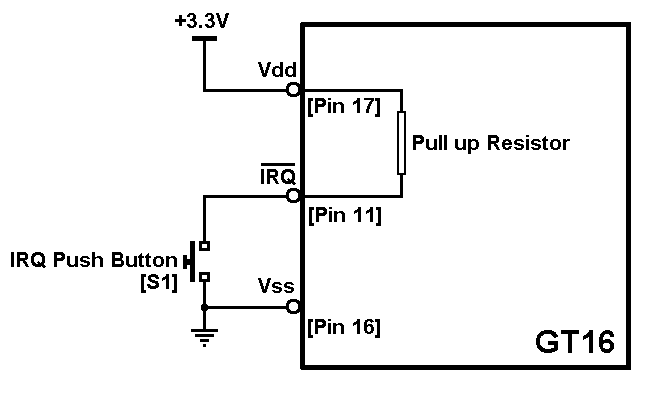
\includegraphics[width=0.7\textwidth]{model.png}
\caption{A block diagram illustrating the connections to the IRQ pin on the MCS08GT16A microcontroller (Please
note that your headings should be short descriptions of what is in the diagram not simply the figure title)}
\label{fig:model}
\end{figure}



\chapter{Rover Model Development Methodology}
\section{Development Objectives}
  \subsection{Problem Definition}
  The project aims to support science education and outreach, leveraging the modern technologies of today, through the development of a working, scaled down version of the \textit{Curiosity} rover. The project brief indicated that the typical use case as desired by the client was to have the rover simulate chosen, significant features of the rover on Mars to shed some light on the level of capability of space technologies that are currently in operation. The model will be set either in a simulated Martian environment or in a small display area and is required to be remotely controllable, providing video and telemetry to viewers and viewer's devices the same way the \textit{Curiosity} RSVP would to the flight team at JPL.
  
  As an initiation of the project, the requirements were explored and collated below into a list of those pertaining to the vehicle itself in a sense of the hardware as well as the software that encompassed the operation of the vehicle. The requirements made as little reference to technologies available as possible as this detail was to be further developed after analysis of the requirements on a functional level.
  
  \subsection{Project Requirements}
  \label{subsec:probDef-projectRequirements}
  \begin{enumerate}
    \item Develop and build a model of the Mars \textit{Curiosity} rover. The rover model should:
    \begin{enumerate}
      \item\label{enum:req-scaledrover} be a scaled down representation of JPL's rover currently operational on Mars with a level of resemblance adequate for use in a realistic exhibit. In other words, it should have been realistic enough such that someone who might have seen a picture of \textit{Curiosity} beforehand could identify the rover,
      \item have traversal capabilities that reflect those on \textit{Curiosity},
      \item be able to make use of these traversal capabilities on uneven terrain such as one which would be a simulated surface as part of the exhibit without resulting in an unrecoverable state,
      \item offer video streaming to connected clients
      \item have reasonable awareness of obstacles to prevent resulting in an unrecoverable state as well as to provide an indication of the navigational and environmental awareness systems on \textit{Curiosity},
      \item have data communication facilities available to best represent the communication systems and subjects of those that are a part of MSL, and
      \item be completely wireless, again reflecting the nature of operation of \textit{Curiosity}.
    \end{enumerate}
    \item Develop a software system to accompany the above rover in its functioning. The software system should:
    \begin{enumerate}
      \item be able to receive data in the form of video and telemetry from the model,
      \item be able to present the data received to users or operators in an interactive manner on a platform that is readily available and accessible,
      \item allow input of commands or control by the users in a manner which is both friendly to a wide range of audiences and age groups and as closely representative of the manner in which JPL's flight team would do so,
      \item transmit these commands to the model to be executed, and
      \item facilitate the reception and transmission of the above data wirelessly.
    \end{enumerate}
  \end{enumerate}
  
  \subsection{Analysis of Constraints}
    As with any engineering design project, the rover development was faced with multiple constraints that affected the resulting design. Below is a brief list of the constraints known at the beginning of the project.
    
    \begin{itemize}
      \item Typical exhibition space limited to a dimension of 3m x 3m
      \item Availability and access to 3D printing facilities
    \end{itemize}
    
    ![Fill out]
    
  \subsection{Functional Analysis}
    The client requirements as highlighted in the previous sub-section were analysed to develop a functional outline in lieu of developing a list of specifications. This analysis served as the starting point for the componentization of the project, allowing for the conceptual development to follow the breakdown. This is discussed further in the next section. Here, each of the requirements, and combinations of them, were used to result in a breakdown of functions and aspects. A significant effort was made from the start of the project to develop the rover in a modular fashion. This is not to be confused with the outcome being modular (although this was still a desirable feature) but is instead the way in which ideas were formed and developed. The functions outlined in this analysis were treated as modules, where possible, and developed so that each module had as little dependence in operation as possible on another. Following this mindset allowed for the simplification of the design process and the robustness of what was developed against constraints and unforeseen obstacles during development.
    
    The current manner in which the requirements were formulated distinguished clearly the two aspects of the project which inevitably became the two major points of development. Both aspects, the mechanical vehicle and the software system, and their differing natural design approaches made it suitable to discuss them separately, where appropriate. The specifications indicated the possibility of a subset of \textit{Curiosity's} primary functions being included in the model. The requirement of a video feed as well as simulated terrain traversal implied there be at least the mast subsystem, which included the moving head components, and a functioning wheel and suspension system that could be controlled. The ability to drive the rover as well as point the camera via motion of the head component was deemed a combination of functions that would contribute well towards providing an engaging experience for the users. These two systems drove the inclusion of the accompanying systems and components, a breakdown of which can be seen in Figure~\ref{fig:specs-functionalBreakdown}.
    
    \begin{figure}[h]
      \centering
      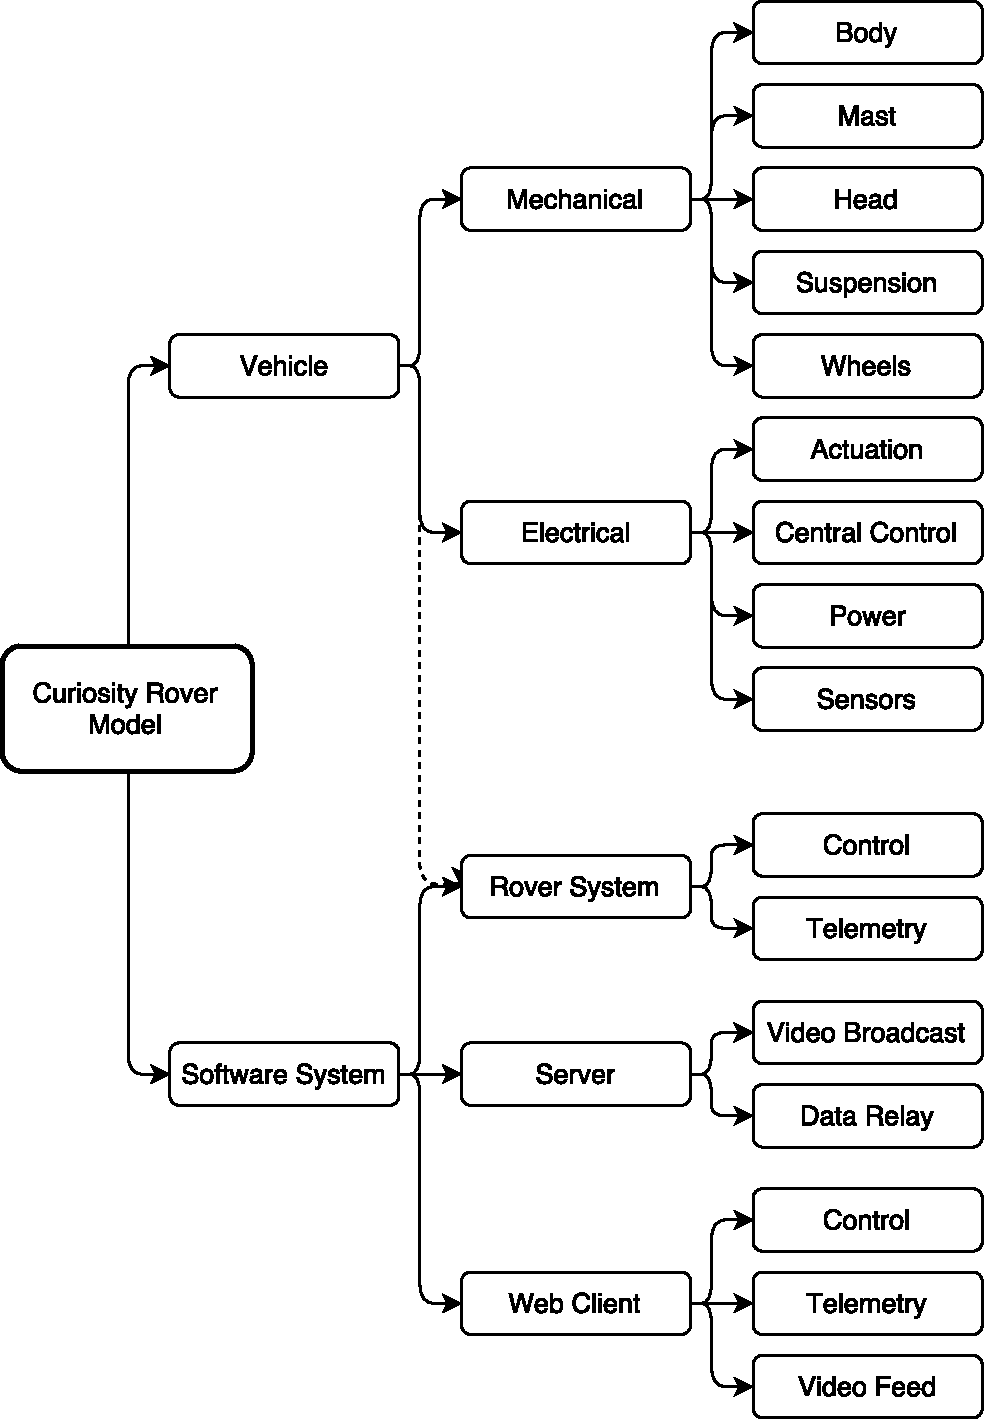
\includegraphics[width=0.6\textwidth]{figures/specs-functionalBreakdown}
      \caption[High-level breakdown of functional entities of the project]{High-level breakdown of functional entities of the project}
      \label{fig:specs-functionalBreakdown}
    \end{figure}
    
    \subsubsection{Rover Equivalence and Terminology}
    \label{subsubsec:rover-equivalence}
      Following the educational theme of the project, much of the terminology used on \textit{Curiosity} was borrowed for use in subsystems and components on the model, in both mechanical and software aspects.
      
      ![Fill out]
    
    
  \subsection{Technical Specifications}
    The technical specifications were derived from the client requirements and the functional analysis, with knowledge of the systems and subsystems on \textit{Curiosity} (taken from review of literature as covered in Chapter~\ref{chap:lit-review}. The specifications further compartmentalised the vehicle and software systems as evident in the structure of them in the lists that follow. These technical specifications served as the baseline requirements for the final design.
    
    \subsubsection{Vehicle Specifications}
    \label{subsec:probDef-vehicleSpecifications}
      \begin{itemize}
        \item \textbf{Mechanical}
        \begin{RM}
          \item General Specifications:
          \begin{RM}
            \item Be as dimensionally accurate as possible to the Curiosity rover on Mars
            \item\label{li:probDef-spec-mechanical-realism} Exhibit a satisfactory level of realism and external aesthetic accuracy
          \end{RM}
          \item Body:
          \begin{RM}
            \item Box shaped
            \item Allow mounting of the mast and differential on the top surface
            \item Allow mounting of the suspension system on either side
            \item Allow mounting of additional sensors
            \item Allow mounting of additional detail such as side panels and other mockup objects
            \item Allow mounting of electrical internals
            \item Provide protection/coverage of electrical internals from the external environment
          \end{RM}
          \item Mast:
          \begin{RM}
            \item Provide mount point for the head module
            \item Facilitate full rotation about the $z$-axis (camera panning/yaw axis)
            \item Facilitate at least $120^\circ$ degrees rotation about the $y$-axis (camera pitching axis)
            \item Be structurally secure providing robustness against lateral forces on the mounted head module
          \end{RM}
          \item Head:
          \begin{RM}
            \item Be mounted onto the mast module
            \item Provide mount point for a sensor
            \item Allow mounting of a camera module
          \end{RM}
          \item Suspension:
          \begin{RM}
            \item Ensure body stability
            \item Maintain stability despite uneven terrain. This includes terrain which might require asymmetrical articulation of the system (a rock underneath one side of the rover and flat terrain underneath the other)
          \end{RM}
          \item Wheels and Hubs/Pivots:
          \begin{RM}
            \item Match the shape and proportion of the wheels on \textit{Curiosity}
            \item Provide traction required for an analogue Martian terrain
            \item Have steering capabilities which would amount to arc pattern traversal as well as rotation of the rover around a central fixed point
          \end{RM}
        \end{RM}
        
        \item \textbf{Electrical}
        \begin{RE}
          \item Actuation:
          \begin{RE}
            \item Provide continuous rotational actuation for driving. The actuation speed should be controllable and must be of high enough torque to satisfy traversal specifications
            \item Provide sufficient magnitude rotational actuation for turning of the wheels for steering. The rotational position should be controllable and must be of high enough torque to facilitate turning of the wheels in-place
            \item Provide required magnitude rotational actuation for panning and pitching of the head/mast module. Both axes must allow positional control
          \end{RE}
          \item Central Control:
          \begin{RE}
            \item Host onboard software system for control of hardware
            \item Facilitate wireless communications with the server
            \item Interface with actuation and sensory input hardware
            \item Have performance capabilities sufficient for processing and streaming of video data from the head module
          \end{RE}
          \item Power:
          \begin{RE}
            \item Provide power for the central control hardware as well as actuation and sensor hardware components
            \item Power supply unit must fit inside or on the body module
            \item Have the ability to be turned switched off or on
            \item Allow convenient removal of source
            \item Allow easy access to charging ports
            \item Provide a means of indication of voltage for telemetry and low-battery warnings
          \end{RE}
          \item Sensors:
          \begin{RE}
            \item\label{li:probDef-spec-sensors-immediateObstacleData} Provide immediate environment data required to implement elementary obstacle detection and avoidance
            \item Be mounted in locations similar to those on \textit{Curiosity}
            \item Be compatible with the central control module in terms of data interface
          \end{RE}
          \item Camera:
          \begin{RE}
            \item Facilitate a monoscopic video feed
            \item Be mountable inside the head module
            \item Be compatible with the central control module in terms of data interface
          \end{RE}
      \end{RE}
    \end{itemize}
      
    \subsubsection{Software System Specifications}
      \begin{itemize}
        \item \textbf{Rover Embedded Software}
        \begin{RS}
          \item General Specifications:
          \begin{RS}
            \item Allow connection of a remote client for telemetry and control as well as another for video streaming
            \item Be robust against hardware errors and intermittent communication so as to maintain operation in these circumstances
          \end{RS}
          \item Control:
          \begin{RS}
            \item Provide a programmatic means to peripheral hardware access
            \item Translate control input commands into hardware output signals for control of peripheral hardware components
            \item Declare/define and execute programmatic sequences facilitating procedures such as system booting, communication initialisations, hardware initializations, self diagnosis and emergency modes
          \end{RS}
          \item Telemetry:
          \begin{RS}
            \item Emit system telemetry to the connected client consisting of system, process and hardware state as well as sequence execution notifications
          \end{RS}
          \item Video Stream:
          \begin{RS}
            \item Provide a stream of the video data to the connected client
            \item Provide video resolution on or above VGA (640$\times$480) resolution
          \end{RS}
        \end{RS}
        
        \item \textbf{Server}
        \begin{RS}[resume]
          \item General Requirements:
          \begin{RS}
            \item Manage communication with the rover system
            \item Manage communication with the connected web clients
            \item Serve web application to the connected web clients
            \item Manage roles of the connected web clients with respect to their level of access and ability to control the rover
          \end{RS}
          \item Video Broadcast:
          \begin{RS}
            \item Connect to and accept video data from the rover video stream
            \item Broadcast video stream to a scalable number of connected user clients
            \item Be robust against communication intermittency in terms of connection with the rover system
          \end{RS}
          \item Data Relay:
          \begin{RS}
            \item Relay control input commands from a controlling web client to the rover
            \item Provide a means of simulating long-distance communication 
            \item Relay telemetry data from the rover system to the connected web clients
            \item Relay state information of the rover system and server system to the connected web clients
          \end{RS}
        \end{RS}
          
        \item \textbf{Client}
        \begin{RS}[resume]
          \item Control:
          \begin{RS}
            \item Provide two means of control of the rover, if access is granted:
            \begin{enumerate}
              \item RoSE-style command sequence input, allowing composition of a sequence of commands and playback of such commands
              \item Interactive joystick/button interface
            \end{enumerate}
          \end{RS}
          \item Telemetry:
          \begin{RS}
            \item Accept and display telemetry received from the rover via the server and from the server itself
          \end{RS}
          \item Video Feed:
          \begin{RS}
            \item Accept and display video feed received from the broadcast
          \end{RS}
        \end{RS}
      \end{itemize}
\section{Conceptual Design and Development}
  It was clear from the composed list of specifications that both electrical and mechanical aspects of the project required development of a large number of parts. In a typical conceptual design process, one could propose a number of complete concepts (i.e. incorporating all aspects of the project) and then make a judgement based on analysis of these concepts. For this project, it was decided that each of the subcomponents outlined in the specifications be conceptually envisioned separately with consideration of neighbouring or related subcomponents and the compatibility between each. Analysis was then undertaken for each of the subcomponents and a final design was composed in a convergent manner, taking the best concept from each of the analyses.
  
  The fact that the design of \textit{Curiosity} off which this model was based helped to maintain structure during a highly parallel, componentised conceptual development. However, the majority of the software components and some hardware components relied on the design of other components therefore the design process was not \textit{entirely} parallel. In fact, in the case of the vehicle development, it was due to it being largely a process of replication that most of the conceptual development involved material and manufacture design choices as opposed to brand new conceptual ideas that required analysis of design feasibility.
  
  \subsection{Rover Concept Proposals}
  \label{subsec:rover-concept-proposals}    
    \subsubsection{Body}
      All of the proposed ideas for the body component of the model revolved around the idea of a hollow box structure. The box was required to host electronics but at the same time, provide structural stability for all other components that were to be mounted to it. Therefore, the choice here was between the materials from which it would be built.
      
      \subheading{Concepts}
      \begin{enumerate}
        \item \textbf{Carbon Fibre:} The first idea envisioned the use of carbon fibre to form a box structure that could be very thin and light but still offer the required strength. The carbon fibre would be cured around a mould made from another rigid, easy to use material. When rigid, holes would be drilled for mounting components and electronics. This concept includes the use of fibre glass which is commonly interchanged with carbon fibre. Both materials offer similar tensile strength, however, carbon fibre is far more robust in flexure \cite{fibreGlast_2016}.
        
        \item \textbf{Perspex/Acrylic Sheet Assembly:} The next idea involved creating the box by designing and cutting panels from acrylic sheet of acceptable thickness, and later fusing the panels to form the structure. Cut-outs could have been included in the design together with holes for shafts and mounting points, which may also have been drilled after the fact. Internal support structures could have been included if the strength of the bonds or of the structure in general was in question due to the fact that acrylic sheet offers high flexibility. Figure~![] shows an example of how the panels might be assembled.
        
        ![Perspex concept render]
        \item \textbf{3D Printing:} One of the aims of the project was to develop the model with high realism in an attempt to make the use of the simulator an engaging and appealing experience. The idea of 3D printing the box structure was considered and it would have allowed for a large degree of detail to be included at little additional effort or cost. Most features such as mounting points (those beyond just holes) and aesthetic detail could have been designed on top of base and internal structural support. A material could have been chosen which might offer the required rigidity, however, due to the nature of the manufacturing process, specifically the reliance on heat for the deforming of the plastic filament in the printing process, 3D printed components would not provide the same strength and robustness as compared to that of the other concepts. A 3D model of the rover created and published by NASA was found which was intended for 3D printing. Of specific interest was the body component which shows the detail that is achievable with this method a render of which is in Figure~![].
        
        ![Figure of 3D nasa body model]
        
        \item \textbf{Milled Aluminium:} Aluminium was another concept that was considered due to its easier manipulative qualities (compared to those of steel) as well as significant reductions in weight. The box structure could have been milled from a block to form the hollow structure that is required, using CNC technology. Holes for mounting and a fair degree of aesthetic detail, which may not have lived up to that achievable by 3D printing means, may have been possible as well. Having the box structure made from aluminium would have meant that threaded holes for mounting would have been possible, eliminating the need for full-stack fasteners.
      \end{enumerate}
      
      \subheading{Discussion}\\\\
      All of the above concepts were achievable, however, each drew on very different material requirements and manufacturing techniques. Carbon fibre moulding and setting was seen as being a potentially difficult process in terms of ensuring an accurate outcome as it relied on a larger degree of manual manufacturing input. It was also the only idea that required extra components to be manufacture in support, namely the mould around which it would have been formed. The other three concepts allowed for more direct CAD-to-finished-product processes and the automation involved in the manufacture of them meant higher accuracy and less manual input. Since the model was small in scale, a design choice discussed further on in this report, strength of components and the weight of other components was far less of a priority as compared to resistance to heat and level of detail.
      
      \subheading{Comparative Analysis}\\\\
      Table~\ref{tab:concept-compAnalysisBody} shows the weighted comparative analysis of the body concepts.
      
      \begin{table}[H]
      \centering
      \begin{tabular}{@{}L{0.3\textwidth}C{0.12\textwidth}C{0.12\textwidth}C{0.12\textwidth}C{0.12\textwidth}C{0.12\textwidth}@{}}
      \toprule
      Attribute & Weight & Carbon Fibre & Acrylic Sheet Assembly & 3D Printing & Milled Aluminium \\ \midrule
      Ease of Manufacture & 5 & 1 & 5 & 3 & 4 \\
      Cost of Manufacture & 4 & 4 & 5 & 3 & 4 \\
      Duration of Manufacture & 5 & 4 & 5 & 3 & 4 \\
      Cost of Material & 4 & 2 & 4 & 3 & 3 \\
      Weight & 5 & 5 & 5 & 4 & 2 \\
      Tensile Strength & 2 & 4 & 3 & 3 & 5 \\
      Modulus & 3 & 5 & 4 & 4 & 1 \\
      Achievable Detail & 3 & 1 & 1 & 5 & 4 \\
      Achievable Accuracy & 3 & 1 & 3 & 4 & 5 \\ \midrule
      \multicolumn{2}{r}{\textbf{Total}} & 2.735 & \textbf{4.147} & 3.353 & 3.324 \\ \bottomrule
      \end{tabular}
      \caption{Comparative analysis of the body component concepts}
      \label{tab:concept-compAnalysisBody}
      \end{table}
    \subsubsection{Suspension System}
      The suspension system of the rover was a critical part with respect to the traversal requirements. It was decided up front that the system replicate the feature as it was on \textit{Curiosity} in both appearance and in operation. The Rocker-bogie mechanical principle employed for the \textit{Curiosity's} suspension system was simple and robust and therefore made clear the decision to use the principle in the model as well. The design problem here was more concerned with the structure and material of the joints as well as how they would be fitted with the beams/rods that links the system together. Another design consideration was that of the differential cross-beam that was mounted to the top of the \textit{Curiosity} which articulated around a center point. The choice of differential bar was dealt with in a separate analysis.
      
      All of the concepts imply the use of shafts and bearings for free articulation between each of the rocker-bogie sections.
      
      \subheading{Concepts}
      \begin{itemize}
        \item \textbf{Fully 3D Printed Assembly:} In this concept, all the parts were to be 3D printed in full. This meant that the joints and beams of the suspension system were not separate pieces, lowering the number of pieces required to be manufactured. Since the suspension system was the largest load bearer compared to that of the other subsystems, the fully printed pieces could have been reinforced with an aluminium or steel rod set down the center of the beam sections. The reinforcements could have extended partially into the joint section of each piece, as the most amount of structural risk would have been at the point where the joint and the beam meet.
        
        \item \textbf{Printed Joints with Aluminium Tubing:} Instead of printing the entire system, an option of printing the joints only and fitting them with aluminium tubing, as the beams, was considered. 3D printing provides the benefit of being able to materialise complex objects which may contain features which conventional manufacture methods might not be able to accomplish, thus making it well suited to the unique nature of the joints in the suspension system. The beams, however, were standard in shape and would not have put this benefit to use, hence motivating the suitability of a light but strong product such as aluminium tubing. The joints would have been designed either to have the tubing fit into the joint, or have a plug onto which the tubing could be pressed.
      
        ![Render of an example plug joint and alu]
      
        \item \textbf{Sheet Brackets with Aluminium Tubing:} This concept built on the previous concept with the joints being made from sheet metal bent into bracket-type shapes onto which the tubing could have been fastened (by means of clamps). The bending process would have allowed for formation of the non-conventional angles that the suspension system required.
        
        ![Render of an example sheet bracket]
        
        \item \textbf{Milled Aluminium Joints with Aluminium Tubing:} Again, instead of the 3D printed joints or the sheet metal, this concept made use of milling aluminium to form the joint structures and having aluminium tubing be fitted into these joints. The milled joints would have been able to offer more surface area to features such as mounting points for the tubes and bearings, meaning that these parts would be more secure. This idea was borrowed from the OpenCuriosity project![] as highlighted in Section~\ref{chap:lit-review}.
        ![Image of the machined joint of OpenCuriosity]
      \end{itemize}

      \subheading{Discussion}\\\\
      The fully 3D printed concept was appealing in that it offered the most direct path from CAD design to the finished product but had much reduced structural qualities as opposed to that of the other concepts. Using a combination of tubing and manufactured joints made sense in terms of the nature of the features and aluminium tubing provided strength beyond what was required, at least as far as the tubing itself was concerned. Brackets made from sheet metal may have offered the best weight (that is, the lightest weight contribution) but required extra manual manufacture as well as would not have been suited to mounting bearings and the tubes whilst maintaining mount rigidity. Both milled aluminium and 3D printed joints solved this problem with the ability of being able to provide more rigidity for fastening tubes and fitting bearings. However, milled joints were bound in structure to the block of aluminium from which they were to be milled, meaning that in one particular plane, the axes of the joints would not have been able to be angled such as required by the suspension design.
      
      \subheading{Comparative Analysis}
      \begin{table}[H]
      \centering
      \begin{tabular}{@{}L{0.3\textwidth}C{0.12\textwidth}C{0.12\textwidth}C{0.12\textwidth}C{0.12\textwidth}C{0.12\textwidth}@{}}
      \toprule
      Attribute & Weight & Full 3D Print & 3D Printed Joints w/ Tubing & Sheet Joints w/ Tubing & Milled Joints w/ Tubing \\ \midrule
      Ease of Manufacture & 5 & 4 & 3 & 2 & 3 \\
      Duration of Manufacture & 3 & 2 & 4 & 5 & 3 \\
      Cost of Manufacture & 4 & 2 & 3 & 4 & 3 \\
      Cost of Material & 4 & 3 & 4 & 5 & 4 \\
      Weight & 4 & 4 & 4 & 3 & 2 \\
      Link Mount Rigidity & 5 & 3 & 4 & 1 & 5 \\
      Aesthetic Accuracy & 3 & 5 & 5 & 1 & 3 \\
      Suitability for Wheel Mounts & 4 & 5 & 5 & 4 & 5 \\ \midrule
      \multicolumn{2}{r}{\textbf{Total}} & 3.500 & \textbf{3.938} & 3.031 & 3.563 \\ \bottomrule      
      \end{tabular}
      \caption{Comparative analysis of the suspension system concepts}
      \label{tab:concept-compAnalysisSus}
      \end{table}
      
    \subsubsection{Differential System}
      The differential system comprised of a beam or arm that articulated about a center point on the top surface of the body and linkage mechanisms connecting the ends of the arm to the rocker pivot point on either side's suspension system. Due to the motion of the differential, strength was only required in the horizontal plane which gives reason for the thin, flat design of that on \textit{Curiosity}. The linkages on the ends of the bar required hinges with two degrees of freedom, the detail of which is discussed further on in this report. Once again, the principle of operation of this subsystem was taken from \textit{Curiosity} itself and therefore was not the design choice to be made here.
      
      \subheading{Concepts}
      \begin{itemize}
        \item \textbf{Acrylic Sheet Bar with Steel Cord Linkage:} Since the differential bar was required to take forces in the horizontal plane, the bar did not have to be round and a conceptual idea involved cutting out the flat bar from acrylic sheet. The acrylic sheet would have been thick enough such that it be press fitted onto a bearing and shaft in the center of the body deck. The ends of the differential would then have been connected to the extensions on the main suspension joint by means of steel cord. The cord would have allowed for the degrees of freedom required given the interface between the differential bar and the suspension and each of their component axes of motion.
        
        \item \textbf{3D Printed Bar with 3D Printed Hinge Pieces:} Instead of cutting the bar from acrylic sheet, this concept envisioned the bar being 3D printed. The linkages would have also been 3D printed as two parts per hinge bolted together and each end of the hinge (one at the suspension and one on the differential bar) would be joined together using threaded bar, secured by use of fasteners.
      \end{itemize}
      
      \subheading{Discussion}\\\\
      Since the acrylic sheet is already flat, it suits the problem well and is easier in terms of manufacture compared to a 3D printed version. Holes for the bearings and the hinges on the ends of the bar could be included in the cutting process. Two sheets could have been glued together to form a thicker beam in the case that the bearing was thicker than the sheet. The 3D printed version, however, would have been of designed thickness thus allowing custom fitting for the bearing. Although steel cord was considered given it's flexibility and thus ability to cater for the ranges and axes of motion of either ends of the linkage, it was shortly dismissed given that it would have only been able to provide support in tension and not in compression. A fixed threaded bar, as proposed in the second concept, provides support in both tension and compression situations, therefore meeting the requirements. Threaded bar was chosen for easy fastening as well as providing the ability to adjust the extension of the linkage for fine tuning the balance of the suspension-differential system and ultimately the balance of the rover. In any case, a weighted comparison was still made in Table~\ref{tab:concept-compAnalysisDiff} since the 3D printed hinges were still compatible with the idea an acrylic sheet differential.
      
      \subheading{Comparative Analysis}
      \begin{table}[H]
      \centering
      \begin{tabular}{@{}L{0.3\textwidth}C{0.12\textwidth}C{0.2\textwidth}C{0.2\textwidth}@{}}
      \toprule
      Attribute & Weight & Acrylic Sheet Bar w/ Steel Cord Linkage & 3D Printed Bar w/ Printed Hinge Pieces \\ \midrule
      Ease of Manufacture & 5 & 5 & 3 \\
      Duration of Manufacture & 3 & 5 & 2 \\
      Cost of Manufacture & 4 & 4 & 3 \\
      Cost of Material & 4 & 5 & 3 \\
      Weight & 3 & 5 & 4 \\
      Strength & 5 & 3 & 5 \\
      Mountability & 5 & 3 & 5 \\
      Linkage Motion & 4 & 0 & 4 \\
      Linkage Support & 5 & 5 & 5 \\
      Aesthetic Accuracy & 2 & 1 & 4 \\ \midrule
      \multicolumn{2}{r}{\textbf{Total}} & 3.575 & \textbf{3.900} \\ \bottomrule      \end{tabular}
      \caption{Comparative analysis of the differential concepts}
      \label{tab:concept-compAnalysisDiff}
      \end{table}
      
    \subsubsection{Wheel Hubs and Pivots}
      The center wheels were fixed in rotation about the $z$-axis and thus the mounting features of these two wheels were included in the suspension system as in the previous concept section. The front and rear wheel pairs, however, were required to rotate in order to provide steering to the rover and therefore had to accommodate for this rotation as well as actuation components for this motion. The wheel pivots were also required to be attached to the suspension system.
      
      The concepts developed for these components followed very similar concepts to those of the suspension hinges as they offered the same principles of articulation and mounting. The final decision would therefore be in accordance to the suspension system final design.
      
    \subsubsection{Wheels}
      The wheels on \textit{Curiosity} are signature features in aesthetics as well as, of course, in function. The wheel shape includes the characteristic curved cross-section which has benefits for terrain like that on Mars and are unique in the thinness of their outer surface or skin. It was noted that the relative strength of the wheels on the scaled model that was being developed would be required to be significantly less than on \textit{Curiosity} and so the design choice here was based primarily on the resulting aesthetic accuracy as the wheels would serve as a great feature in which to fulfil the client requirement of the model being highly realistic.
      
      \subheading{Concepts}
      \begin{itemize}
        \item \textbf{3D Printed Wheels:} The fact that the wheels had the distinct shape that they did meant that 3D printing them would render highly accurate representations in terms of their shape on those of \textit{Curiosity}. The design would include holes and points at which shafts and/or bearings could be fitted without the need for drilling or any other type of post-produce manipulations.
        
        \item \textbf{Off-the-shelf RC Wheels:} Another option was to purchase read-made wheels and tires intended for use on radio-controlled cars. The wheels would have points for mounting by default and would offer the benefits of a rubber tire over that of plastic. Once again, this idea was borrowed from the OpenCuriosity model in ![]. The project indicated that this method was successful in function.
      \end{itemize}
      
      \subheading{Discussion}
         While the 3D printed wheels would have offered less structural robustness as ready-made wheels designed to endure high impact, gravel environments, there was no requirement for the model to traverse any faster or in any better manner than \textit{Curiosity} and thus the added benefit of the rubber tires and strong wheels would be an over-design. Although the RC wheels would have had points at which shafts could be fitted, and potentially even bearings already installed, this would impose limitations on the size of the shafts chosen. In the case of the 3D printed wheels, holes sizes could have been chosen to work with materials and bearings that were available.
         
      \subheading{Comparative Analysis}
        \begin{table}[H]
        \centering
        \begin{tabular}{@{}L{0.3\textwidth}C{0.12\textwidth}C{0.2\textwidth}C{0.2\textwidth}@{}}
        \toprule
        Attribute & Weight & 3D Printed Wheels & Off-the-shelf RC Wheels \\ \midrule
        Ease of Manufacture & 3 & 3 & 5 \\
        Duration of Manufacture & 4 & 2 & 5 \\
        Cost of Manufacture & 4 & 3 & 2 \\
        Cost of Material & 4 & 3 & 2 \\
        Weight & 1 & 5 & 2 \\
        Traction & 3 & 3 & 5 \\
        Terrain Suitability & 3 & 4 & 5 \\
        Mount-type Flexibility & 4 & 5 & 2 \\
        Aesthetic Accuracy & 5 & 5 & 1 \\ \midrule
        \multicolumn{2}{r}{\textbf{Total}}  & \textbf{3.613} & 3.097 \\ \bottomrule
        \end{tabular}
        \caption{Comparative analysis of the wheel and tire concepts}
        \label{tab:concept-compAnalysisWheel}
        \end{table}
      
    \subsubsection{Neck and Head}
      The mast of the model required rotation about the $z$-axis and a joint about which an additional axis of rotation was possible to result in two degrees of freedom for the head component. \textit{Curiosity} employed a hinge mounted to the bottom of a second, smaller box structure, the head, which rotated to provide camera pitch. The pitch actuation mechanism was situated atop a second mechanism which provided actuation for pan-axis rotation. The size of \textit{Curiosity} allowed smart fitting of the motors in-line with the mast shaft and embedded in the head mount hinge, however, the scaled model was not able to accommodate for motors in this way. ![Put this in the detailed design, concept designs are meant to be somewhat ideal!] It was decided that it be acceptable for the mast assembly to be out of proportion, visually, in order to be able to fit the required actuation (the component choices of which were largely based on availability).
      
      \subheading{Concepts}
      \begin{itemize}
        \item \textbf{Aluminium Tube Mast with 3D Printed Fittings:} This concept made use of aluminium tubing (the same material as in the suspension system concepts) which would be set and fastened into the body. A 3D printed plug with mounting points for the camera-pitch actuation mechanism would have been designed to fit into the top of the tube, as can be seen in Figure~\ref{fig:concepts-aluMast}. Camera-pan actuation would have been built into the inside of the body into which the mast tube would extend. The height of the head could therefore have been adjusted since the tube was free-moving with respect to the rover deck.
        
        \begin{figure}[H]
          \centering
          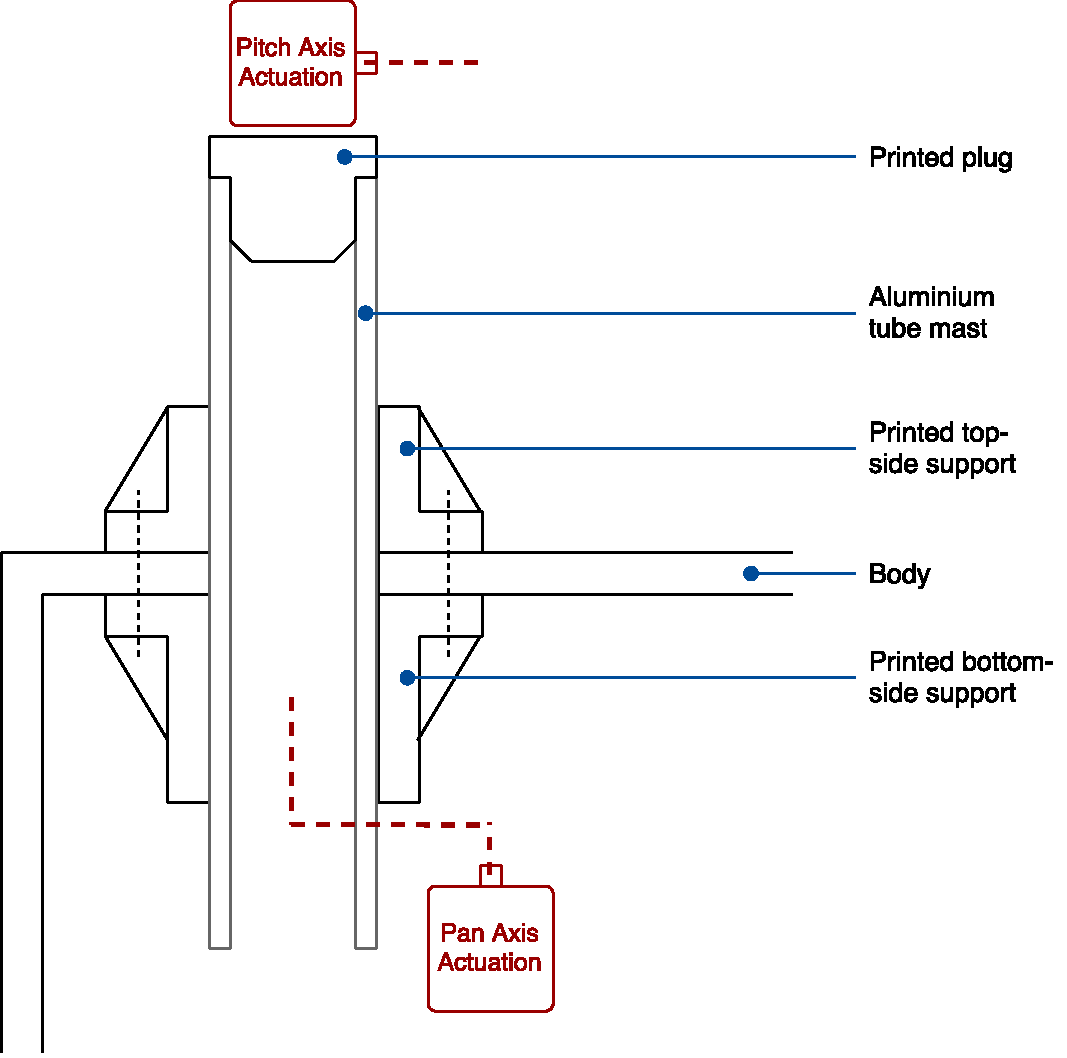
\includegraphics[width=0.7\linewidth]{figures/concepts-aluMast}
          \caption[Conceptual diagram of a section view of the body and aluminium mast assembly]{Conceptual diagram of a section view of the body and aluminium mast assembly}
          \label{fig:concepts-aluMast}
        \end{figure}
        
        \item \textbf{Full 3D Printed Assembly:} As opposed to making use of the aluminium tube, this concept employs 3D printing for the full assembly which would be mounted to the top of the rover body with no portion of it extending below the deck. The camera-pan actuation would be the same as in the previous concept but the camera-pitch actuation mechanism would be brought above the level of the rover deck. Further, an actuation mechanism that combines both axes of motion could ave been developed to reduce the spatial footprint that it might have incurred. The width of the base of the mast, at the mounting point, would be increased to provide structural support.
        
        \begin{figure}[H]
          \centering
          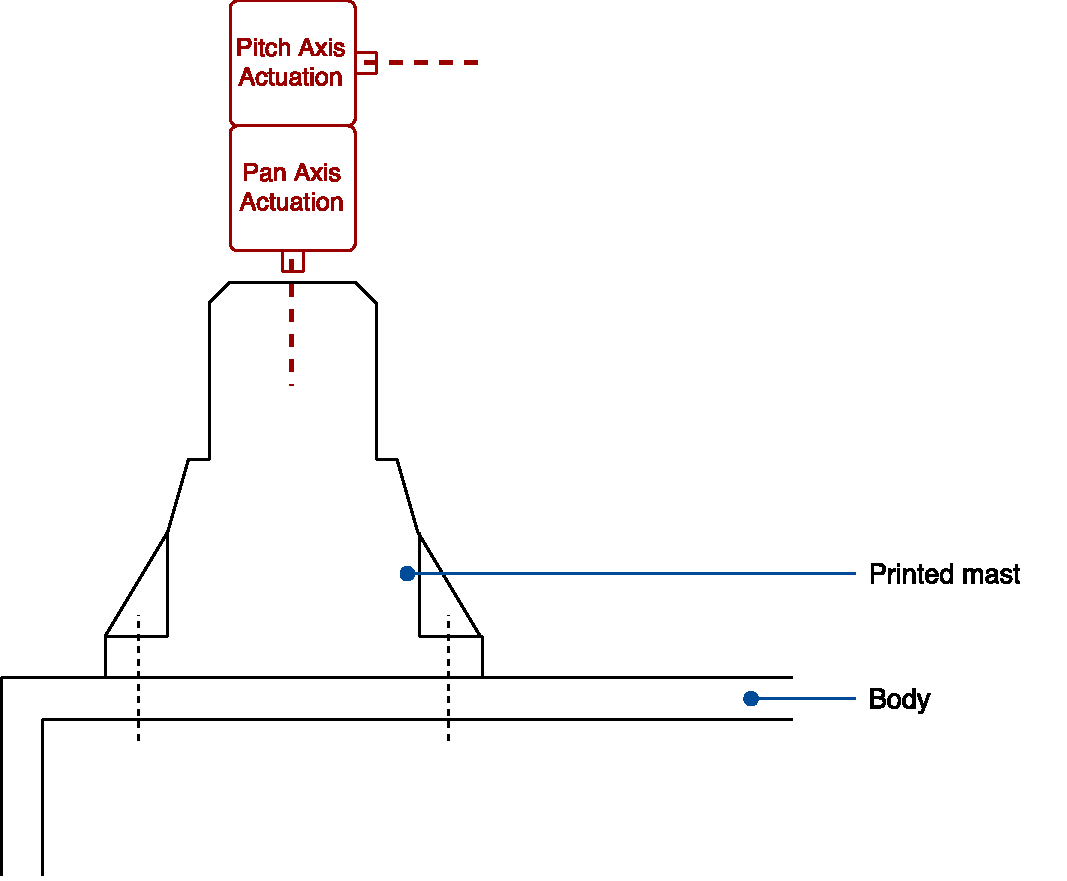
\includegraphics[width=0.7\linewidth]{figures/concepts-printedMast}
          \caption[Conceptual diagram of a section view of the body and printed mast assembly]{Conceptual diagram of a section view of the body and printed mast assembly}
          \label{fig:concepts-printedMast}
        \end{figure}
        
      \end{itemize}
      
      \subheading{Discussion}\\\\
        Positioning one of the two component actuation mechanisms inside the body had benefits for the spatial footprint above the rover deck, however, the implications of taking up more space inside the body were far greater given the intended use of that area. Having the entire tube mast rotate within the opening hole from below the deck might have increased the torque requirements on the actuation mechanism, dependant on the nature of the opening. The intended use of the opening was to provide structural support and any fit tolerance introduced to improve the torque requirements of the actuation would negatively impact the effectiveness of the hole feature in its support function. This could have been solved with a bearings, however, that would have incurred addition room for mounting.
      
      \subheading{Comparative Analysis}
        \begin{table}[H]
        \centering
        \begin{tabular}{@{}L{0.3\textwidth}C{0.12\textwidth}C{0.2\textwidth}C{0.2\textwidth}@{}}
        \toprule
        Attribute & Weight & Aluminium Tube w/ 3D Printed Fittings & Full 3D Printed Assembly \\ \midrule
        Ease of Manufacture & 3 & 2 & 4 \\
        Duration of Manufacture & 4 & 4 & 3 \\
        Cost of Manufacture & 4 & 3 & 3 \\
        Cost of Material & 4 & 4 & 2 \\
        Weight & 4 & 3 & 4 \\
        Proportion & 3 & 4 & 3 \\
        Body External Footprint & 3 & 4 & 3 \\
        Body Internal Footprint & 5 & 1 & 5 \\
        Strength & 5 & 5 & 4 \\ \midrule
        \multicolumn{2}{r}{\textbf{Total}} & 3.200 & \textbf{3.514} \\ \bottomrule
        \end{tabular}
        \caption{Comparative analysis of the wheel and tire concepts}
        \label{tab:concept-compAnalysisMast}
        \end{table}
      
    \subsubsection{Actuation}
      All components requiring actuation mechanisms have been covered in the above concepts. Consisting of only rotational motion requirements, the mechanisms were split into two categories based on the desired order of output motion (translated from the desired order of input control signal), namely angular position and angular velocity. Position actuation was required for rotating the wheels about their $z$-axis pivot for turning or steering and to provide panning and pitching motion to the head subsystem with the camera. Both of the functions involved setting a desired angular position and having the mechanism hold that position during operation. On the other hand, driving the wheels of the rover was better thought as involving an output velocity. \textit{Curiosity} made use of high-ratio motors for all types of rotational actuation to ensure robustness of the design, higher torque outputs and to achieve precise control of each of the driven features which was acceptable in that high-speed performance was not a targeted requirement.
      
      \subheading{Concepts}
      \begin{itemize}
        \item \textbf{High Torque DC Motors:} Using high torque DC motors would have been the most accurate replication of the actuation as used on \textit{Curiosity}, as each of the mechanisms had high-ratio gearboxes attached to the brushless motors. The DC motors would have been controlled by means of PWM which would have resulted in an output angular velocity. For this reason, a control loop mechanism would have to be employed for positional motor control in the case of the subsystems that required it.
        \item \textbf{Analog RC Servos:} A candidate alternative to using high torque DC motors that was considered was servos, intended for radio-control vehicle use, into which a high-torque gearbox was already built. An example of this type of motor is shown in Figure~\ref{fig:concepts-servoMotorExample}. The motors operated using a pulse signal of which the width translated to a specific position as a percentage of the motor's rated angular range.
        
        \begin{figure}[H]
          \centering
          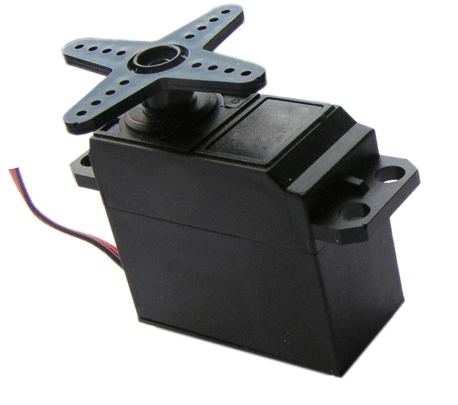
\includegraphics[width=0.3\linewidth]{figures/concepts-servoMotorExample}
          \caption[Image of an example of an RC servo motor]{Image of an example of an RC servo motor \cite{fig:concepts-servoMotorExample_cite}}
          \label{fig:concepts-servoMotorExample}
        \end{figure}

      \end{itemize}
      
      \subheading{Discussion}\\\\
        The two candidate actuation devices were in fact similar in that they both offered high torque output, however, the inclusion of a built-in analog position control system differentiated the servos from the DC motors. If the DC motors were to be used, the central system would had to provide an external control system to implement position control for the head and mast subsystem as well as the pivoting of the wheels. Further, this would have required output state capture by means of an encoder or an analog-to-digital converter adding complexity to the system. The fact that the servos had this control functionality built in meant this solution would have greatly reduced the incurred complexity of the actuation of the rover as a whole, as all that would have been required is for the system to provide a power rail and PWM signals.
        
        The choice of actuation mechanisms was highly dependant on the chosen combination of subsystem concepts, specifically that of the power supply, the central control system and those that needed actuation themselves. No weighted comparison was performed for the above concepts as the choice was heavily affected by these subsystems.
    
    \subsubsection{Central Control System}
    \label{subsubsec:central-control-system}
      The central control system was a critical component not only to the rover, but to the conceptual design process as it was an enabler/disabler of many of the candidate solutions. Discussed here are the electronic hardware comparisons made with respect to the central control system. The software design process took on a secondary priority approach and as such, the hardware choices were driving of the design (not without consideration of implications in the software system). As will be mentioned in full in the detailed design section, it was intended to follow a COTS design approach as far as possible given the time-frame of the project as well as the notion of keeping the design open to others who might be familiar with the hardware components chosen with respect to the aim of open sourcing. As far as education and outreach is concerned, familiar hardware is well suited to helping users and those involved in the project learn the principles of a rover design.
      
      Conceptual candidate systems included popular, small, single-board computers, sized appropriately with the intention of fitting the system in the body of the model. Note that the lower-level device class suited to deeper embedded software applications was considered and would have proved suitable if it was not for the video streaming requirements. It was anticipated that the video feed would require on-rover encoding and compression and thus imposing the need for a better performing device capable of running a high-level operating system. The requirements for this system, which included wireless communication and embedded interfaces, were kept in mind when performing the comparative analysis. Notable specifications in accordance with the requirements are shown for each of the boards.
      
      \subheading{Concepts}
      \begin{itemize}
        \item \textbf{Raspberry Pi Model B:}
          The Raspberry Pi was a credit-card sized single-board computer which was developed with the intention of aiding computer-science education. It made use of a well-performing CPU as well as an on-chip GPU making it suitable for low-end, media-based computational applications. Raspberry Pi computers have a very large online community from which vast resources were available.
          
          Notable specifications (for the 3rd generation model):
          \begin{itemize}
            \item \textbf{CPU:} 1.2 GHz 64-bit ARM Cortex A53 (Broadcom BCM 2837 SoC)
            \item \textbf{Memory:} 1 GB
            \item \textbf{Storage:} None, microSD Card Slot
            \item \textbf{GPIOs:} 40 pins, 
            \item \textbf{Network Connectivity:} Bluetooth 4.1 and Bluetooth Low Energy, 100 Mb Ethernet, 2.4 GHz wireless
            \item \textbf{Other External Interfaces:} 4x USB 2.0, Camera Serial Interface (CSI)
          \end{itemize}
        \item \textbf{Orange Pi:}
          The Orange Pi, an open source variant to the Raspberry Pi, was considered as it offered much the same capabilities as the Rasberry Pi. It was able to run many open source operating systems such as Debian and Ubuntu.
          
          Notable specifications (for the Plus model):
          \begin{itemize}
            \item \textbf{CPU:} 1 GHz 64-bit ARM Cortex A7 (AllWinner H3 SoC)
            \item \textbf{Memory:} 1 GB
            \item \textbf{Storage:} None, microSD Card Slot, SATA 2.0 Connector
            \item \textbf{GPIOs:} 40 pin header, 
            \item \textbf{Network Connectivity:} 1 Gb Ethernet, 2.4 GHz wireless
            \item \textbf{Other External Interfaces:} 4x USB 2.0, Camera Serial Interface (CSI)
          \end{itemize}
          
        \item \textbf{Beaglebone Green Wireless:}
          The Beaglebone Green is another small board as part of the Beaglebone device family, a range of single board computers that have been developed to bridge the gap between embedded electronics and computers. The green version is better suited for embedded applications compared to that of the black version and was the only Beaglebone device that had wireless connection capabilities.
          
          Notable specifications \cite{mouserbeaglebone_2016}:
          \begin{itemize}
            \item \textbf{CPU:} 1 GHz 32-bit ARM Cortex A8 (TI Sitara AM3358)
            \item \textbf{Memory:} 512 MB
            \item \textbf{Storage:} 4 GB eMMC
            \item \textbf{GPIOs:} 65 pins, 
            \item \textbf{Network Connectivity:} Bluetooth 4.1, Bluetooth Low Energy, 2.4 GHz wireless
            \item \textbf{Other External Interfaces:} 4x USB 2.0
          \end{itemize}
          
        \item \textbf{Intel Edison:}
          The Intel Edison is less of a single board computer and more of a complete system on chip mounted to a small board intended for use in the Internet-of-Things industry as well as for mobile and wearable products. The tiny module can further be mounted to a breakout board which provides USB interfaces and a GPIO through-hole grid.

          Notable specifications ![cite]:
          \begin{itemize}
            \item \textbf{CPU:} 400 Mhz Intel Quark x86 (Intel Atom)
            \item \textbf{Memory:} 1 GB
            \item \textbf{Storage:} 4 GB eMMC
            \item \textbf{GPIOs:} 28 pins, 
            \item \textbf{Network Connectivity:} Bluetooth 4, 2.4 GHz wireless
            \item \textbf{Other External Interfaces:} 1x USB 2.0, 1x USB Serial (UART), as provided by the breakout board
          \end{itemize}
 
        \item \textbf{Intel Edison w/ Arduino Breakout Expansion:}
          The Intel Edison had available a second breakout board which was developed to make the SoC compatible with the large variety of Arduino-compatible modules and add-ons.

        \item \textbf{Intel Galileo Gen 2:}
          The Intel Galileo is a development board that better aligns with the single-board computer principle, compared to the Edison. The processor and board are fixed and allows for connection of Arduino-compatible hardware as well as supports a range of other interfaces.
          
          Notable specifications ![cite]:
          \begin{itemize}
            \item \textbf{CPU:} 400 Mhz Intel Quark x86 (Intel Pentium)
            \item \textbf{Memory:} 256 MB
            \item \textbf{Storage:} None, SD Card Slot
            \item \textbf{Network Connectivity:} 1 Gb Ethernet Port
            \item \textbf{Other External Interfaces:} 3x USB 2.0, 1x USB Serial (UART)
          \end{itemize}
      \end{itemize}
      
      \subheading{Discussion:}\\\\
        After careful research into each of the above candidate products, it was decided that all of the boards were suitable for the central computing system of the rover. All of the devices were capable of running high-level operating systems as well as had some means of connecting to a video capture device as well as providing hardware interfaces that might have been required. However, caution was taken to choose a device that would not be over-powered for the application nor provide breakouts and interfaces that would have been left unused. At this point in the design process, it was difficult to determine the exact computational requirements and so the design choice was made based on anticipative measures. It must also be noted that the choice was largely influenced by availability and cost of the devices.
        
        \begin{table}[H]
        \centering
        \begin{tabular}{@{}L{0.15\textwidth}C{0.1\textwidth}C{0.1\textwidth}C{0.1\textwidth}C{0.1\textwidth}C{0.1\textwidth}C{0.1\textwidth}C{0.1\textwidth}@{}}
        \toprule
        Attribute & Weight & R-Pi 3 & Orange Pi & Beaglebone Green Wireless & Intel Edison & Intel Edison w/ Arduino Breakout & Intel Galileo Gen 2 \\ \midrule
        Cost & 5 & 4 & 4 & 3 & 2 & 2 & 1 \\
        \rule{0pt}{2em}Weight & 3 & 4 & 3 & 4 & 5 & 5 & 4 \\
        \rule{0pt}{2em}Availability & 5 & 3 & 1 & 2 & 5 & 4 & 5 \\
        \rule{0pt}{2em}Size & 4 & 4 & 3 & 4 & 5 & 4 & 3 \\
        \rule{0pt}{2em}Wireless Support & 5 & 5 & 5 & 5 & 5 & 5 & 0 \\
        \rule{0pt}{2em}Provision for Video Capture & 5 & 5 & 5 & 4 & 1 & 3 & 3 \\
        \rule{0pt}{2em}Suitability of Processing Power & 3 & 3 & 3 & 3 & 5 & 5 & 3 \\
        \rule{0pt}{2em}Add-on Compatibility & 4 & 3 & 3 & 2 & 1 & 5 & 5 \\
        \rule{0pt}{2em}Power Consumption & 3 & 1 & 1 & 3 & 5 & 4 & 2 \\ \midrule
        \multicolumn{2}{r}{\textbf{Total}} & 3.703 & 3.243 & 3.351 & 3.622 & \textbf{4.000} & 2.811 \\ \bottomrule
        \end{tabular}
        \caption{Comparative analysis of the central control system concepts}
        \label{tab:concept-compAnalysisRce}
        \end{table}

      
    \subsubsection{Camera}
      An important item in the list of requirements and specifications was the capture of a video stream to broadcast to the connected clients. The camera was required to be above VGA resolution ($640\times480$ pixels) and have a means of connecting to the chosen central computing system. The available camera modules were categorised by connector type, listed below.
      
      \subheading{Concepts}
      \begin{itemize}
        \item \textbf{CSI Compatible Webcam:} Many of the central computing system candidates provided support for a Camera Serial Interface (CSI) connected camera for video capture. CSI is a camera interface standard maintained by the Mobile Industry Processor Interface Alliance (MIPI Alliance) that is at its 3rd stage of revision at the time of writing. An example of a CSI camera was the R-Pi Cam, produced specifically for use with a Raspberry Pi.
        \item \textbf{USB Compatible Webcam:} The majority of external webcams were USB connected, allowing them to be easily connected to a laptop or computer. The USB webcams that were investigated as being candidate devices varied in their class of drivers which was a potential issue for compatibility with the central control system, specifically the operating system that would be used. The chosen device, if of type USB, would have had to have been a USB Video Class (UVC) compliant device due to the fact that UVC devices are driverless and thus are compatible with a far greater range of host computers and operating systems.
        \item \textbf{I$^2$C Webcam:} Since the central control system would be capable of allowing serial connections, cameras that were I$^2$C connected were considered.
      \end{itemize}
      
      \subheading{Discussion}\\\\
        The performance benefit of candidate cameras was not possible to determine based on their interface type, but rather the manufacturer and the designed specifications. It was decided that the camera be chosen based on compatibility with the central control system and availability of such a device.
      
    \subsubsection{Proximity}
      ![Fill out]
  
  \subsection{Final Design Choice}
    At this point, the ideas and concepts in Section~\ref{subsec:rover-concept-proposals} had been explored in detail and final choices for each of the subcomponents had been made. This section indicates the outcomes of these choices as well as gives a brief overview of the final concept to be developed. The subcomponent concepts in Section~\ref{subsec:rover-concept-proposals}, shown visually in Figure~\ref{fig:concepts-finalconceptrender}, that included weighted comparisons were finalised primarily by the outcome of those comparisons (i.e. the concept that achieved the highest score, denoted in the Tables~\ref{tab:concept-compAnalysisBody} through~\ref{tab:concept-compAnalysisRce} by bold numbers) and the few that did not follow the same structure of analysis were chosen by compatibility with relevant subcomponents.
    
    \begin{figure}[H]
      \centering
      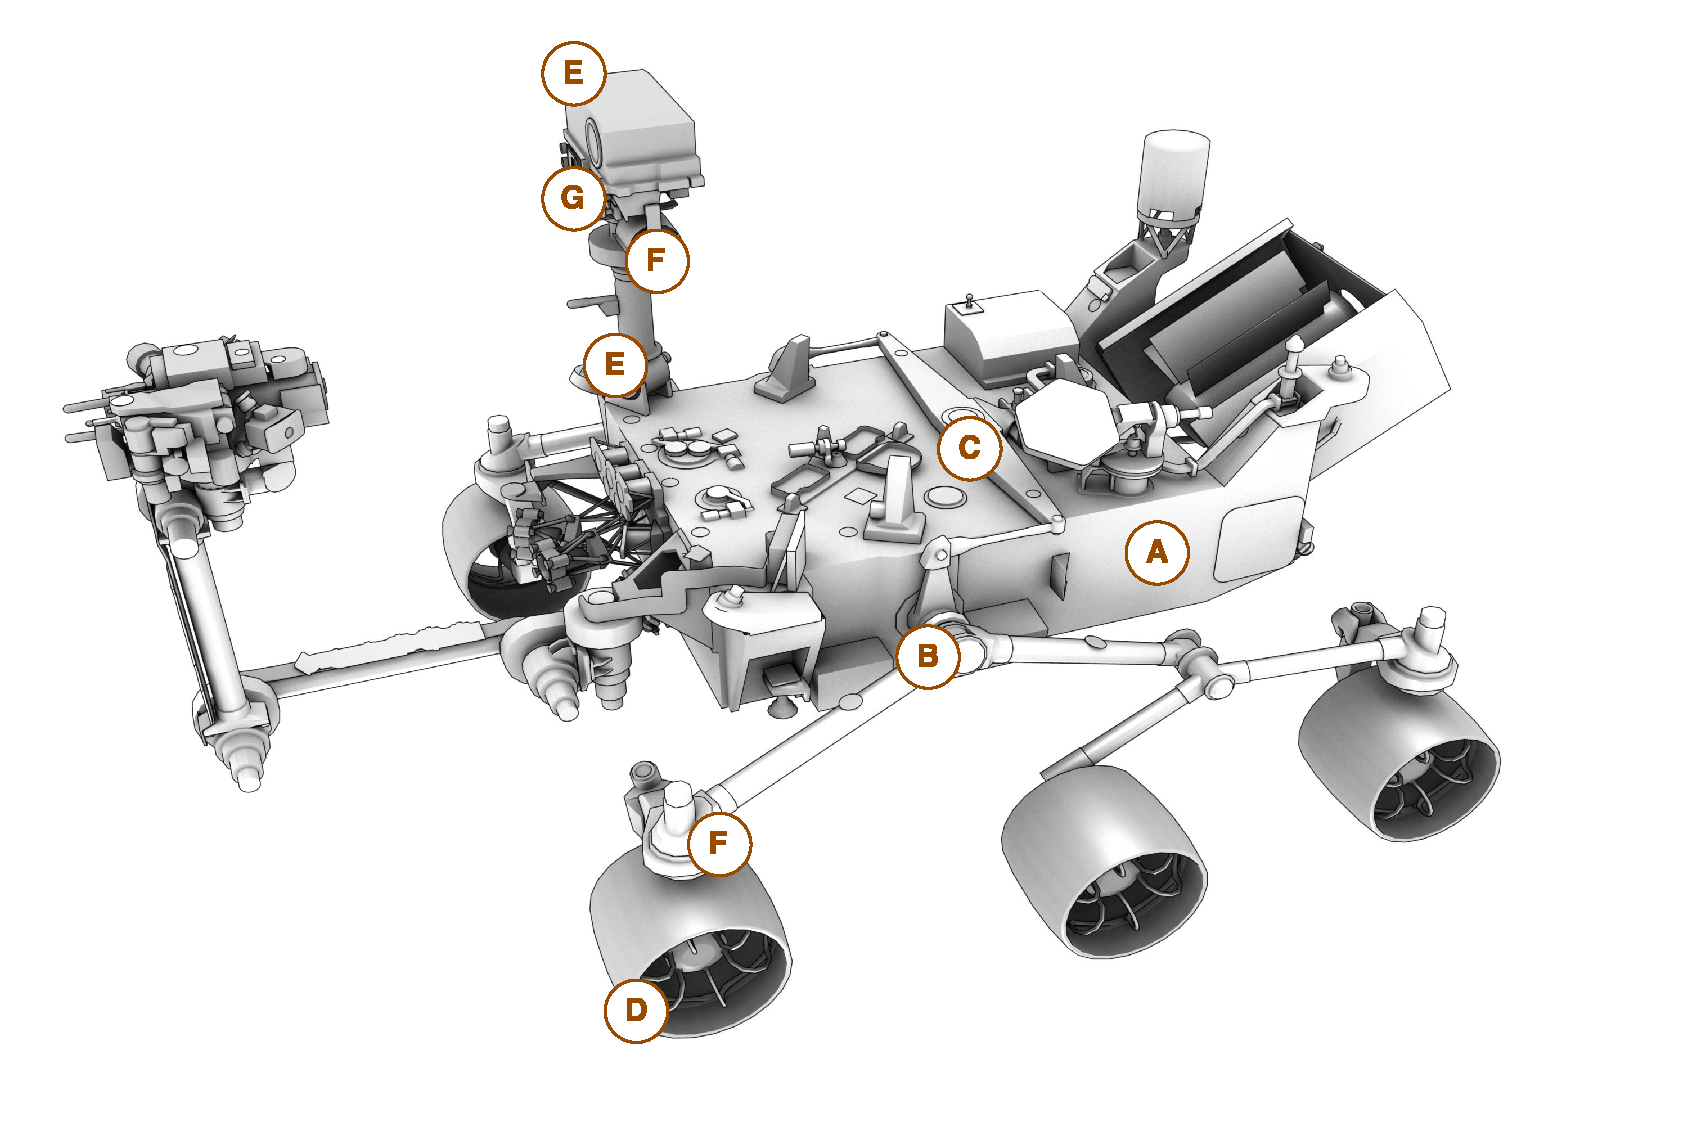
\includegraphics[width=1\linewidth]{figures/concepts-finalConceptRender}
      \caption[Adapted render of a model of the rover indicating the subsystems considered in the conceptual development]{Adapted render of a model of the rover indicating the subsystems considered in the conceptual development \cite{nasa3D}}
      \label{fig:concepts-finalconceptrender}
    \end{figure}
    
    \begin{enumerate}[A.]
      \item It was decided that the body be made from acrylic sheet panels glued together to form the box structure required. The panel design, cutting and assembly was considered easier compared to the manufacturing of carbon fibre and 3D printing as well as being strong enough to provide the central structural support.
      \item The suspension system was to be constructed from 3D printed joints and aluminium tubing for the superior total weight of the assembly and the concept's compatibility with fittings to be made for mounting the wheels. The fact that the joints were to be 3D printed meant that it would become easy to model and print the arbitrary angles of that of the suspension design without the manufacture limitations imposed by other methods and materials. The joints allowed for the design to maintain an accurate representation of that on \textit{Curiosity} without sacrificing function and meant that close fit parts such as bearings could be easily incorporated into the design without imposing constraints on the choice of those types of parts.
      \item A full 3D printed bar with printed hinges was to be used for the differential system due to the acrylic sheet and steel cord not being suitable for the required function. As mentioned in the concept's discussion, the 3D printed differential bar meant that a bearing could be correctly mounted for the motion required. The hinge on the differential bar side would be connected to the suspension side hinge by a threaded bar. As will be discussed, the connecting threaded bar could be used to adjust the distance between the hinges thus providing the ability to finely balance the rover during assembly.
      \item The wheels were to be 3D printed which would allow for superior aesthetic accuracy and custom fit design for bearings and actuation. The 3D printed wheels would be lighter than bought wheels and was deemed worth the incurred manufacture time and cost.
      \item The head and neck (mast) was to be fully 3D printed to make it more suitable to being mounted to the top of the rover deck without any portion of it extending into the body of the rover, taking up space required for the electronics. 3D printing meant the ability to accommodate for the chosen means of actuation. The head would be designed to consist of two parts so that access to the internals of the head was possible. This sub-assembly was then to be mounted to parts connected to the actuation and further parts for mounting on the rover deck.
      \item Choice of actuation settled upon the use of RC servos. The servos were to be of a suitable size, preferably ``sub-micro''\footnote{A ``sub-micro'' servo motor is one of a range of standard sized servos for robotics and radio-controlled vehicle applications}, and compatible in interface with the central control system. The servos chosen were highly geared and were to provide the required torque for actuation of the head and wheels. The servos would have standard mounting holes making incorporation into the design an easier process.
      \item The camera was to be a USB (UVC-compatible) webcam chosen based on availability. The camera would be suitable for use with the chosen central control system and significantly lower in cost compared to the other concept options. It was decided that a webcam be physically altered to be suitable for incorporation into the design of the head.
    \end{enumerate}
    
    Not shown in Figure~\ref{fig:concepts-finalconceptrender} is the central control system, which was to be mounted on the inside of the body structure. The Intel Edison with the Arduino breakout expansion was chosen due to availability of the product as well as its compatibility with add-on hardware, the advantage of which was in the increased development process as a result. The Intel Edison was regarded as being better suited to the performance and computational requirements over the other boards and provided the necessary hardware interfaces for the primary functions and associated hardware for the system throughout.
    
    As discussed in the functional analysis, \textit{Curiosity's} robotic arm subsystem was not included in the model due to time and cost constraints on the project. The design processed aimed to make the addition of this type of a feature possible in potential future work on the project.

    
\section{Vehicle Design and Development}
  Finalisation of the chosen concepts for the development of the rover meant that the project could progress to the detailed design stages. It was discussed in Section~\ref{subsubsec:central-control-system} that the mechanical design of the vehicle would be driving of the overall design, specifically the software aspects, and thus the report will deal with the mechanical and electronic detailed design first.
  
  \subsection{Mechanical Design}
    The mechanical design was initiated by planning the basic layout of mechanical subsystems and components and from that point developing each system further. In this section, the choice of scale (and hence dimensions) is followed by the overall plan of the mechanical layout. Subsystems that are peripheral to the body structure are then covered. These include the suspension, differential and mast subsystems. Finally, the design of the body structure is described as well as detail surrounding the model as a whole.
    
    \subsubsection{Scale and Dimensions}
      Replication of \textit{Curiosity} on an aesthetic level was a project aim to increase the viewers' and users' sense of familiarity with the real \textit{Curiosity} rover, a way of promoting a more engaging experience. The replication process identified that proportion was an effective and achievable starting point and it was decided that as many of the parts as possible be based off the dimensions of the corresponding part on \textit{Curiosity}, brought down to scale by a predetermined factor. Scale was constrained primarily by the cost and manufacturing time of parts that were required to be 3D printed; the larger the model, the greater the amount of material required and the longer it would take to print it. The print bed size was also a constraint in this regard. More details pertaining to the use of 3D printing facilities can be found in Section~\ref{subsubsec:additive-manufacture}.
      
      \begin{figure}[h]
        \centering
        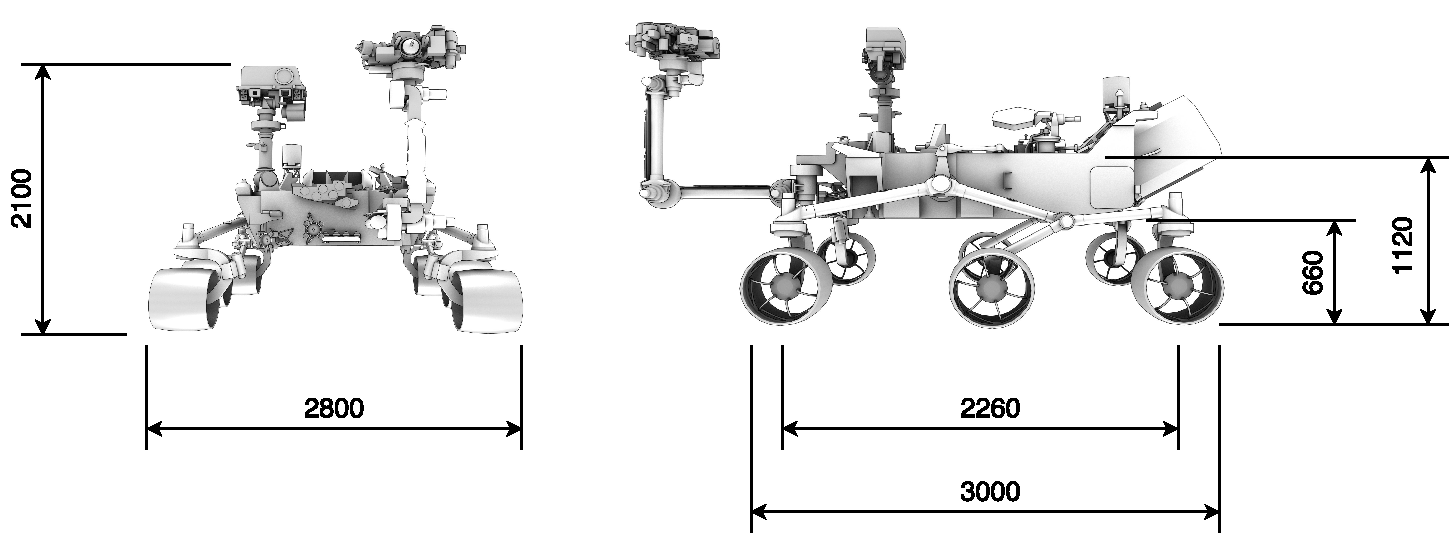
\includegraphics[width=0.9\linewidth]{figures/mechDesign-curiosityDimensions}
        \caption[Diagram indicating the external dimensions of \textit{Curiosity}, in millimetres, these references provided]{Diagram indicating the external dimensions of \textit{Curiosity}, in millimetres, these references provided \cite{nasa3D}}
        \label{fig:mechdesign-curiosityDimensions}
      \end{figure}
      
      The dimensions shown in Figure~\ref{fig:mechdesign-curiosityDimensions} were retrieved from \cite{nasajulypresskit} and \cite{roverThermal_2016} as guidelines. External dimensions only and no other dimensions were available that might have provided a more detailed insight into each of the subsystems and components. A 3D model of a small scale, static, printable model of \textit{Curiosity} published by NASA was found and used for extraction of the 3D proportions of the individual components \cite{nasa3Dprint}. While this model was not ideal in terms of representative accuracy, it provided the much needed basis on which to generate the designs of parts with an acceptable level of similarity. From these details, it was decided that the rover be built at a 1:10 scale, making the total length and width of the model, including the wheels, 300 mm and 280 mm respectively. This scale took into account allowing the model enough space to be used within the typical exhibit size outlined in the problem definition as well as 3D printing capabilities. The scale ensured that anticipated electronic components would fit into the body structure and that mounting of bearings and the chosen standard size of servo motors was reasonable.
      
      The chosen scale gave rise to a set of external dimensions for each of the subsystems, highlighted in Table~\ref{tab:design-referenceDimensions}. The guideline full-scale dimensions in Figure~\ref{fig:mechdesign-curiosityDimensions} were used against the 3D model in \cite{nasa3Dprint}, here-onwards referred to as the reference model, to derive the scale of this reference. This scale was then used to obtain external, high-level dimensions for all of the subsystems and components ensuring that they remained in proportion. In some instances, it was not possible to adhere strictly to the scaling and/or placement of certain components. Such exceptions are discussed in their respective sections.
            
      The reference model, which was in Standard Tessellation Language (STL) format, was imported into a CAD package with millimetre units and evaluated in that state to result in a scale of 1:1.7037 (reference model as to \textit{Curiosity}). The dimensions shown in Table~\ref{tab:design-referenceDimensions} are of priority components and subsystems only, omitting details related to components that were intended to serve aesthetic purposes only (such as a mock-up of the RTG).
      
      \begin{table}[h!]
      \centering
      \begin{tabular}{@{}cccc@{}}
      \toprule
      \textbf{Feature}            & \textbf{Dimension}            & \textbf{Code} & \textbf{Value (mm)} \\ \midrule
      \multirow{3}{*}{Rover}      & Height                        & A1   & 210   \\
                                  & Width                         & A2   & 280   \\
                                  & Depth                         & A3   & 300   \\ \midrule
      \multirow{4}{*}{Body}       & Height                        & B1   & 46    \\
                                  & Width                         & B2   & 136   \\
                                  & Depth                         & B3   & 190   \\
                                  & Ground Clearance              & B4   & 66    \\ \midrule
      \multirow{5}{*}{Suspension} & Height                        & C1   & 122   \\
                                  & Width                         & C2   & 72    \\
                                  & Depth                         & C3   & 271   \\
                                  & Wheel Pitch                   & C4   & 119   \\
                                  & Center-pivot to Body Front    & C5   & 71    \\ \midrule
      \multirow{2}{*}{Wheel}      & Diameter                      & D1   & 50    \\
                                  & Depth                         & D2   & 40    \\ \midrule
      \multirow{5}{*}{Mast}       & Height                        & E1   & 98    \\
                                  & Width                         & E2   & 62    \\
                                  & Depth                         & E3   & 50    \\
                                  & Position from font deck edge  & E4   & 28    \\
                                  & Position from right deck edge & E5   & 28    \\ \midrule
      \multirow{3}{*}{Head}       & Height                        & F1   & 30    \\
                                  & Width                         & F2   & 60    \\
                                  & Depth                         & F3   & 50    \\ \bottomrule
      \end{tabular}
      \caption{Table showing the external dimensions of components and subsystems obtained from the reference model \cite{nasa3Dprint}}
      \label{tab:design-referenceDimensions}
      \end{table}
      
    \subsubsection{Layout Plan}
      The dimensions in Table~\ref{tab:design-referenceDimensions} were used to construct a plan of the layout of subsystems to be used for further detailed design. The plan can be seen in Figure~\ref{fig:mechDesign-layoutPlan}, along with selected dimensions from the Table.
      
      \begin{figure}[h!]
        \centering
        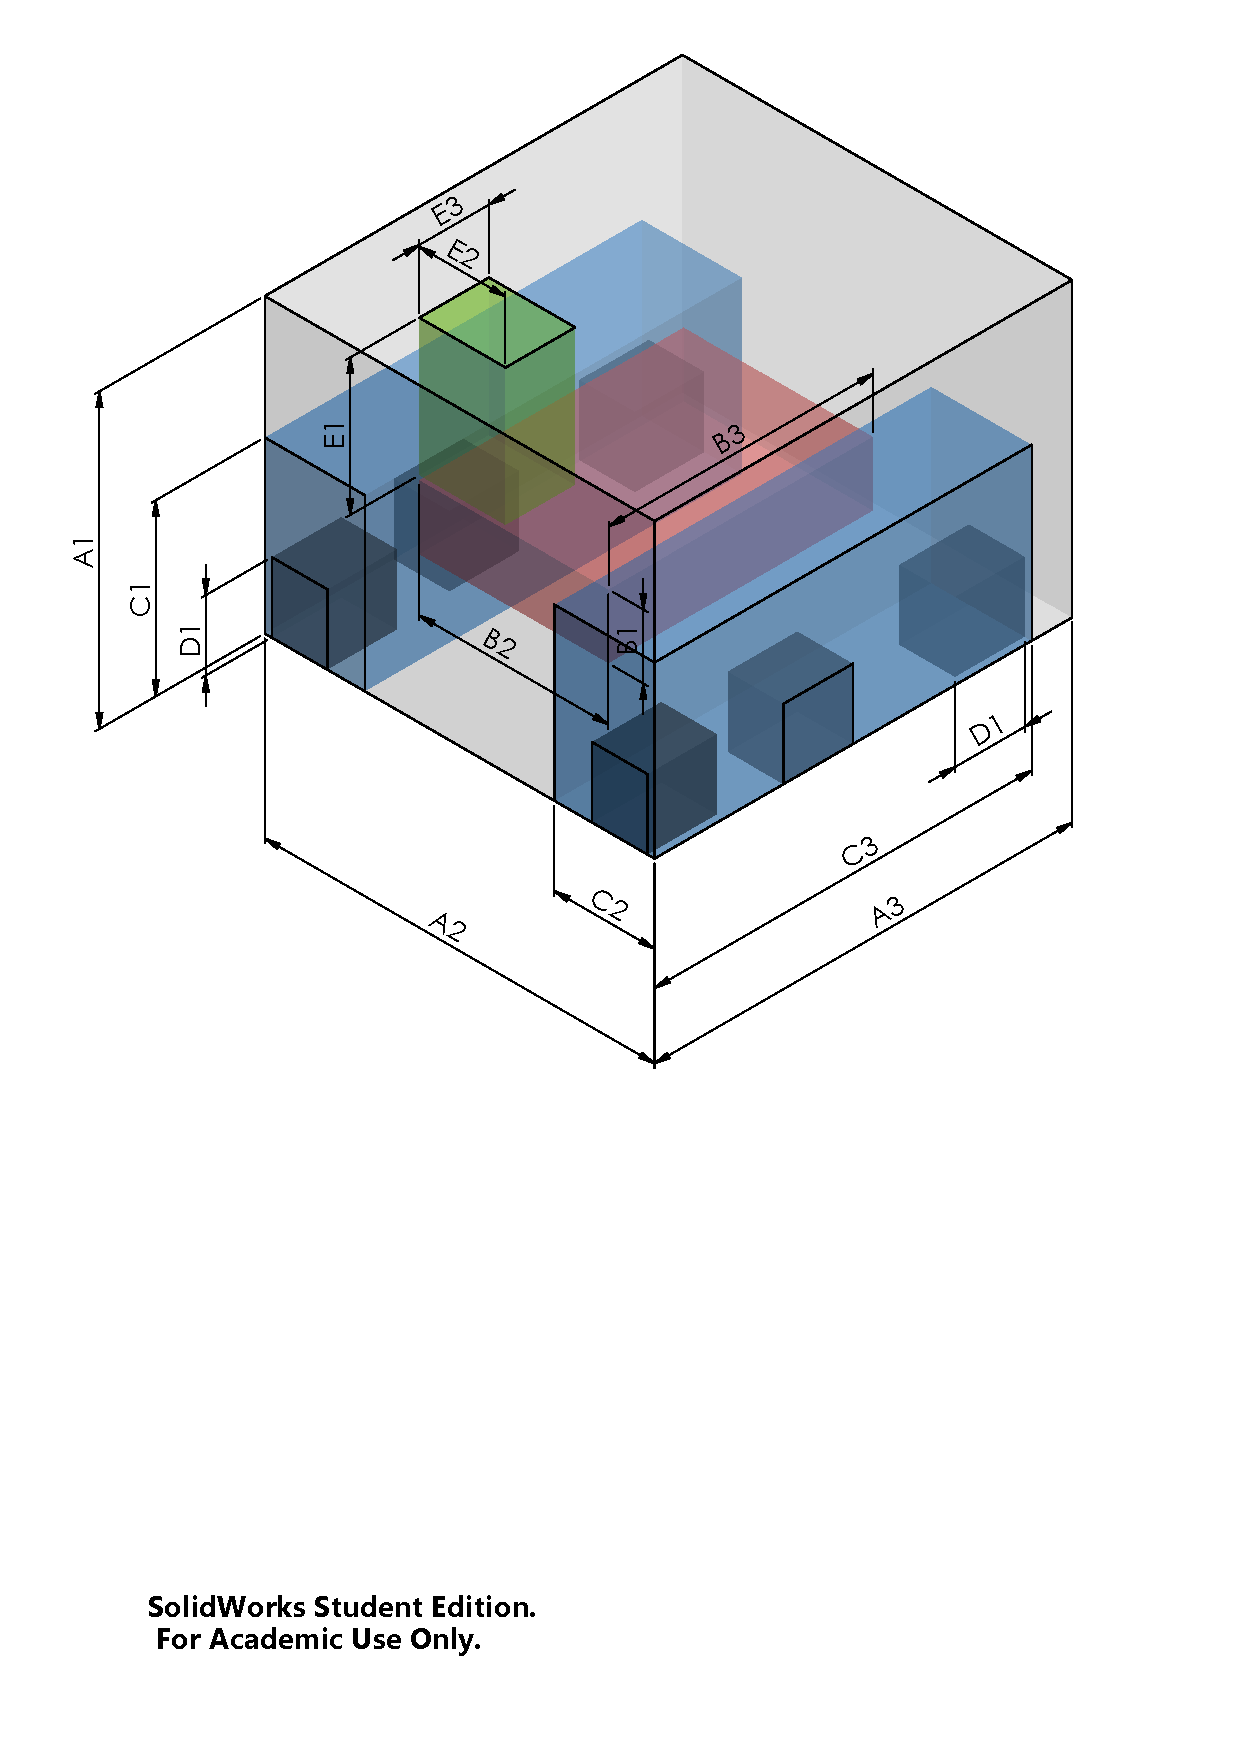
\includegraphics[clip, trim=1cm 11cm 1cm 0cm, width=0.9\linewidth]{figures/mechDesign-layoutPlan}
        \caption[Isometric view of the 3D layout plan of the rover with a subset of the external dimensions shown]{Isometric view of the 3D layout plan of the rover with a subset of the external dimensions shown}
        \label{fig:mechDesign-layoutPlan}
      \end{figure}

      
    \subsubsection{Standard Features}
      Prior to designing and developing the components and parts in detail, standard feature dimensions and sizes were set up to maintain a level of consistency throughout the process. This included features such as holes, walls and fasteners and served as a general guideline allowing for variation of these parameters, if required. Table~\ref{tab:featureStandards} highlights these feature details.
      
      \begin{table}[h!]
      \centering
      \begin{tabular}{@{}llL{0.6\textwidth}@{}}
      \toprule
      \textbf{Feature} & \textbf{Size} & \textbf{Comments} \\ \midrule
      Fasteners & M2 - M3 & Full pan-slotted screw, hex nut and flat washer stack. M3 as first priority dropped down to M2 if the part dimensions or circumstances do not allow. \\ \midrule
      Holes & M2 - M3 & Holes were to match the fasteners in terms of size. \\ \midrule
      Hole Clearances & 0.5 mm & Clearance made to be over a standard fit clearance in anticipation of spread of the surfaces of the part during the 3D printing process. \\ \midrule
      Wall Thicknesses & \begin{tabular}[c]{@{}l@{}}Major: 5mm\\ Minor: 3mm\end{tabular} & Major walls used where significant structural integrity required, whereas minor walls were used both for less significant areas or areas where available space is a constraint \\ \bottomrule
      \end{tabular}
      \caption{Table indicating standards for common features across the entire design}
      \label{tab:featureStandards}
      \end{table}
      
    \subsubsection{Suspension}
      The collection of joints, pivots, struts and wheels was collectively referred to as the suspension system, one positioned on either side of the body structure. Each side of the suspension system included two fixed link mechanisms, the ``rocker'' and the ``bogie'' as part of the ``rocker-bogie'' principle as highlighted in Section~\ref{subsubsec:lit-manoeuvrability}. During the conceptual design phase, it was decided that this mechanism be constructed by connecting aluminium tube pieces to 3D printed joints, on the ends of which the pivots and struts could be attached for the wheels.
      
      The design started with the identification of the components required and a map of how they would be fitted together which included the names of each part for identification throughout the process. Figure~\ref{fig:mechdesign-suspensionLinkageMap} shows this mapping, which can be considered as a lower-level conceptual plan of the system.
      
      \begin{figure}[h!]
        \centering
        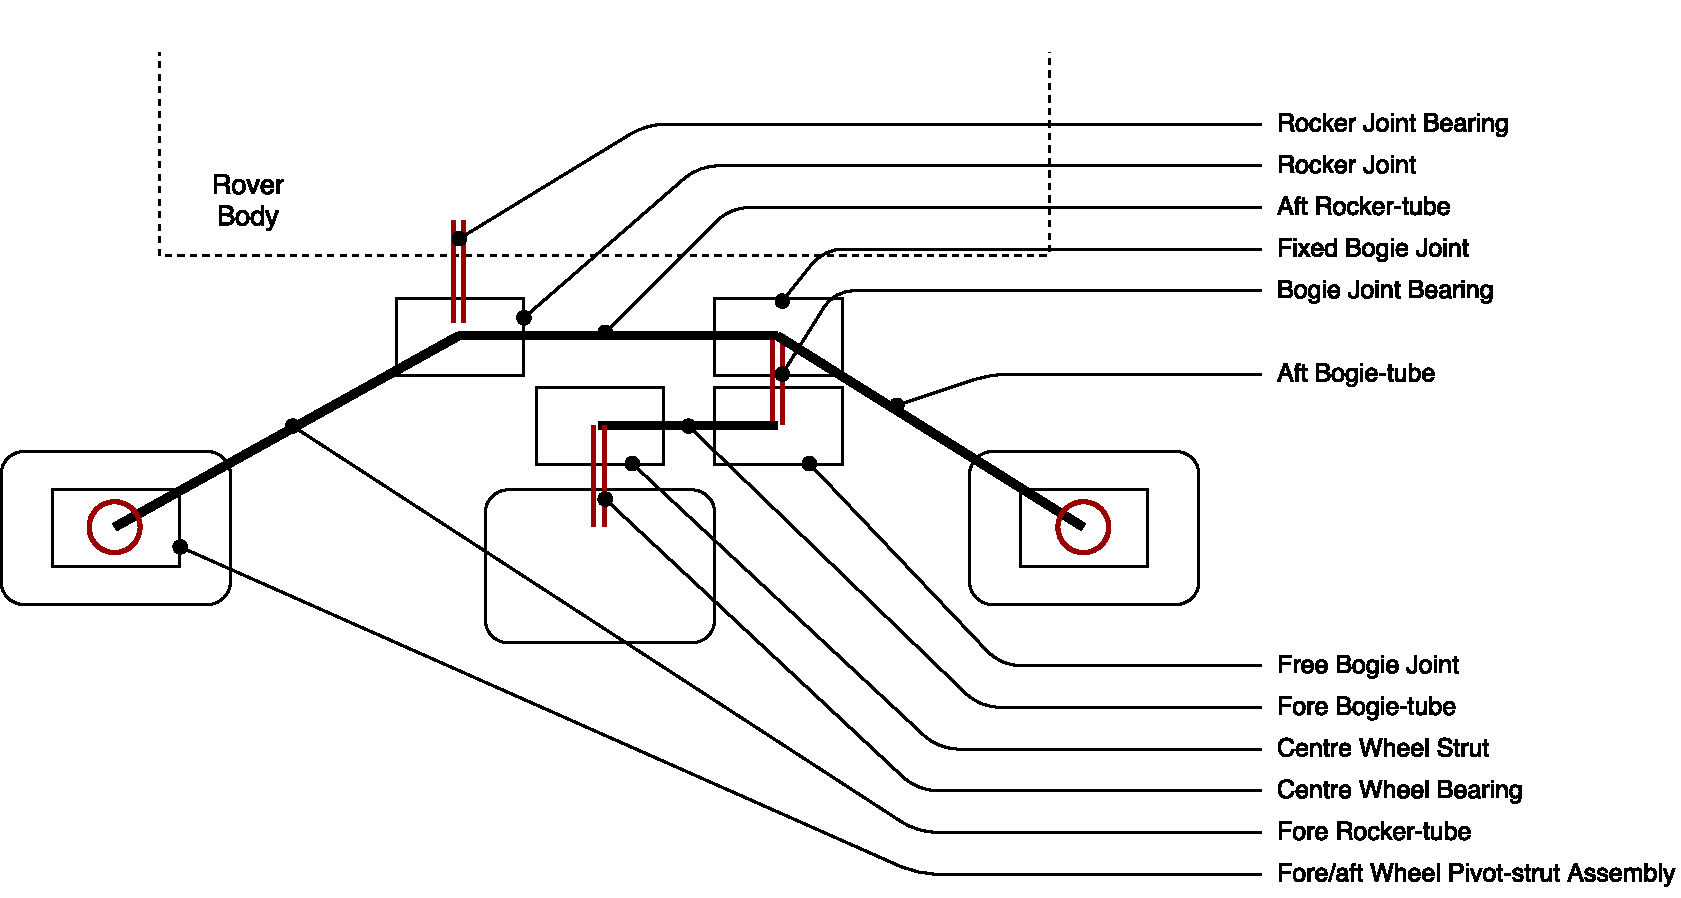
\includegraphics[width=1\linewidth]{figures/mechDesign-suspensionLinkageMap}
        \caption[Schematic diagram of a top view of the suspension system]{Schematic diagram of a top view of the suspension system}
        \label{fig:mechdesign-suspensionLinkageMap}
      \end{figure}
      
      It was noted that the ratios of the tubing or beams on \textit{Curiosity} (and rocker-bogie mechanisms in general) are important since they determine the system's range of motion, affecting the rover's ability to traverse the terrain. The reference model in \cite{nasa3Dprint} was not able to provide this kind of detail, and so the angles and positions of the centre-points of joints and axes of pivots and wheels had to be constructed from reference images of the rover. What was known was the distance of the wheels away from the side of the rover body, that the pivot centre-points were directly above the centres of the wheels and that the aft rocker-tube and the fore bogie-tube were parallel to the body of the rover in the $x$-$y$ plane. Figure \ref{fig:mechDesign-suspensionReferences} includes the images that were used to find these details.
      
      \begin{figure}[h!]
      \centering
      \subfloat[]{
        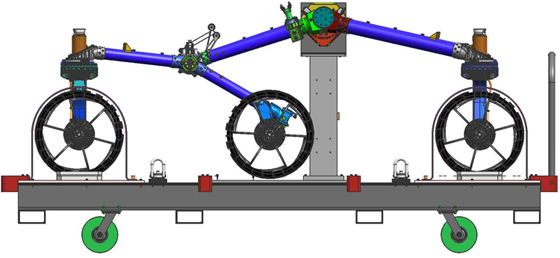
\includegraphics[width=.45\linewidth]{figures/mechDesign-suspensionReference1.jpg}
      }
      \qquad
      \subfloat[]{
        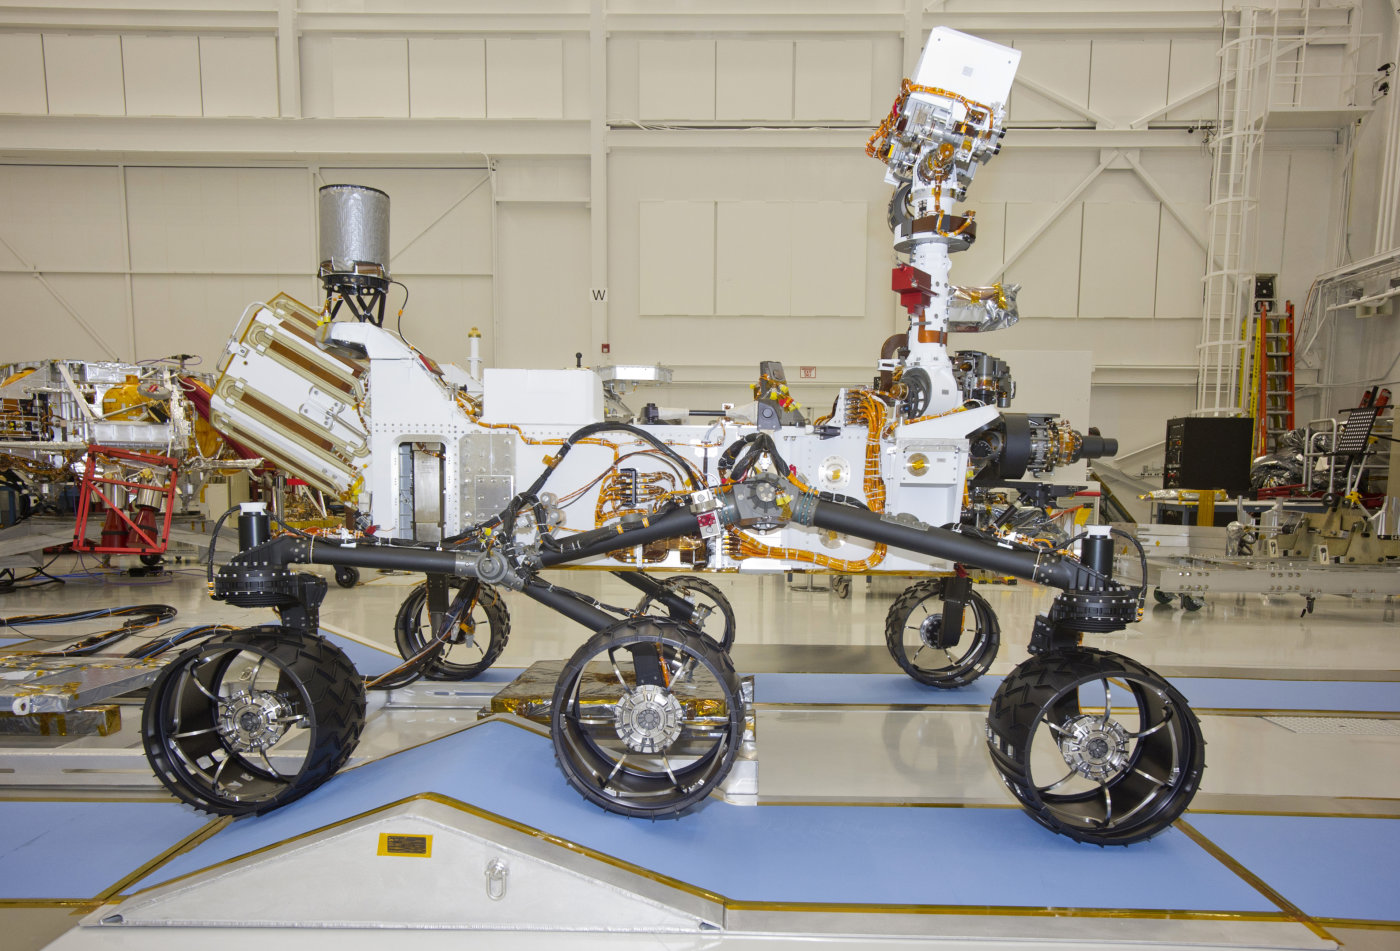
\includegraphics[width=.45\linewidth]{figures/mechDesign-suspensionReference2.jpg}
      }
      \caption[The two images used for obtaining the positions of joints and pivots of the suspension system in 3D space]{The two images used for obtaining the positions of joints and pivots of the suspension system in 3D space. \cite{fig:mechDesign-suspensionReferences1_cite} and \cite{fig:mechDesign-suspensionReferences2_cite}, respectively.}
      \label{fig:mechDesign-suspensionReferences}
      \end{figure}

      A skeleton layout generated from the positional data obtained is shown in Figure~\ref{fig:mechDesign-suspension3d} where a 2D sketch was created as a starting point from which a 3D sketch of the layout was formed. The skeleton sketch was rigid in the position whereby all three wheels were at rest on a flat, horizontal surface parallel to the rover body.
            
      \begin{figure}[h!]
        \centering
        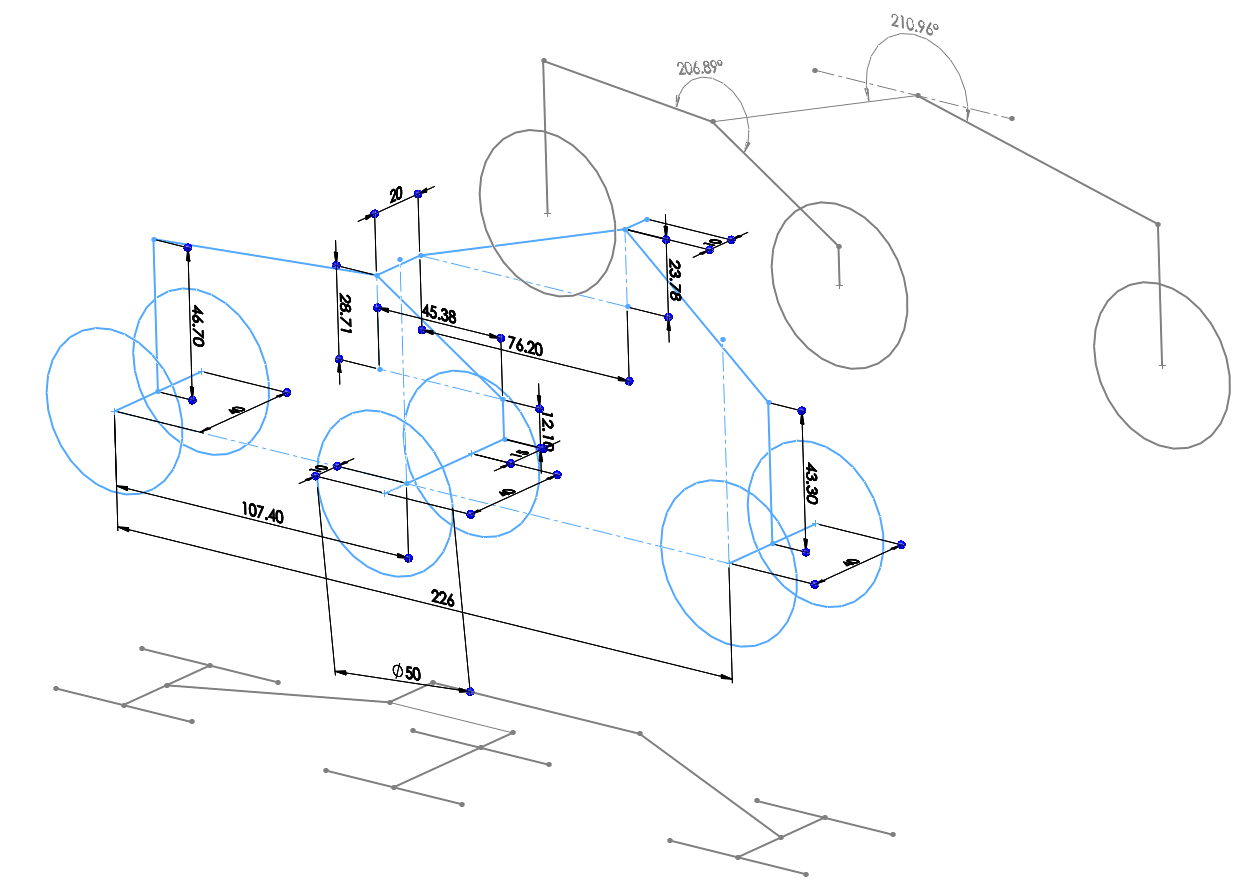
\includegraphics[width=0.9\linewidth]{figures/suspension3D}
        \caption[Isometric view of the 3D sketch of the generated suspension system skeleton used for positioning of designed parts]{Isometric view of the 3D sketch of the generated suspension system skeleton used for positioning of designed parts}
        \label{fig:mechDesign-suspension3d}
      \end{figure}
      
      The joints, pivots and struts were then developed around the axes and centre-points in the sketch, a work-flow typical of the CAD package used.
      
      \subheading{Joints}\\\\
        One side of the suspension system required three different joints: the rocker joint and fixed and free bogie joints. The bogie joints were the simpler of the three and provided a means for the bogie to pivot about one of the ends of the rocker. The fixed joint was fixed in rotation on the end of the rocker while the free joint rotated about a point on the free joint. The rocker joint allows for the entire mechanism to pivot about a point on the side of the rover body as well as allowing attachment of the differential bar in order to keep the two sides of the suspension system coordinated.
        
        It was decided that the rotation of the joints be aided by use of bearings mounted on aluminium shafts. The aluminium would not add excessive amounts of weight to the system but still provide the rigidity required between the joints. Bearings were then required to be fixed into the rocker and free bogie joints with a shaft extending from the side of the body for the rocker joint bearings and another shaft mounted in the fixed bogie joint. Various methods of mounting bearings and shafts into 3D printed parts were considered, however, the most commonly employed technique involved press-fitting both types of components. At this point it was clear that printing the parts from a material which allowed for a certain amount of flexibility (i.e. less brittleness) would suit press-fitting bearings and shafts and reduce the chances of parts cracking when doing so. The press-fit holes and bores were introduced into the design after modelling the joints.
        
        The joints were to host the aluminium tubes and thus a way of mounting them was required. Aluminium tubing dimensions were decided upon based on availability, cost, weight and strength and the aim of keeping the suspension system in proportion was a contributing factor in this design choice. A standard extruded aluminium tube of 15.88 mm outside diameter with a 1.62 mm wall thickness (making the internal diameter 12.64 mm). Two methods of fixing the tubes to the joints were considered, the first of which was to design a plug onto which the tube could be pressed and fastened and the other involved a bracket into which the tube would be placed and the bracket could have been tightened using a clamp or nut and bolt. The plug concept was chosen over the bracket due to size constraints which would have been exceeded if the latter were used. The plugs took advantage of the fact that the aluminium was tubular and minimised use of space outside of the diameter of the tube. However, using a plug might have introduced a weakness into the design in that cross-axis forces (bending moments) on the plug could damage, if not, tear the plug from the joint part. This would not have been the case with a bracket where these types of forces would have translated into forces parallel to the plug main axis. Despite the possible weakness, the plugs were used and care was taken to ensure that typical use would not affect the part in this way. Another reason for not using a bracket was due to anticipation of the plastic material used for the printing possibly deforming when tightened with the suggested fastenings. Plastic, among most other materials, offers greater robustness when compressed (as in an internal plug feature) as opposed to if it is put under tension \cite{makerbotStrength}.
        
        Multiple plug shapes were considered, a range of which are shown in Figure~\ref{fig:mechDesign-plugConcepts}. The aim was to have the plug not require glue, as aluminium is not well suited to being glued using adhesives that work well with plastic parts. An ideal plug was one where just the press-fitting process was satisfactory in order to obtain a rigid attachment.
        
        \begin{figure}
        \centering
        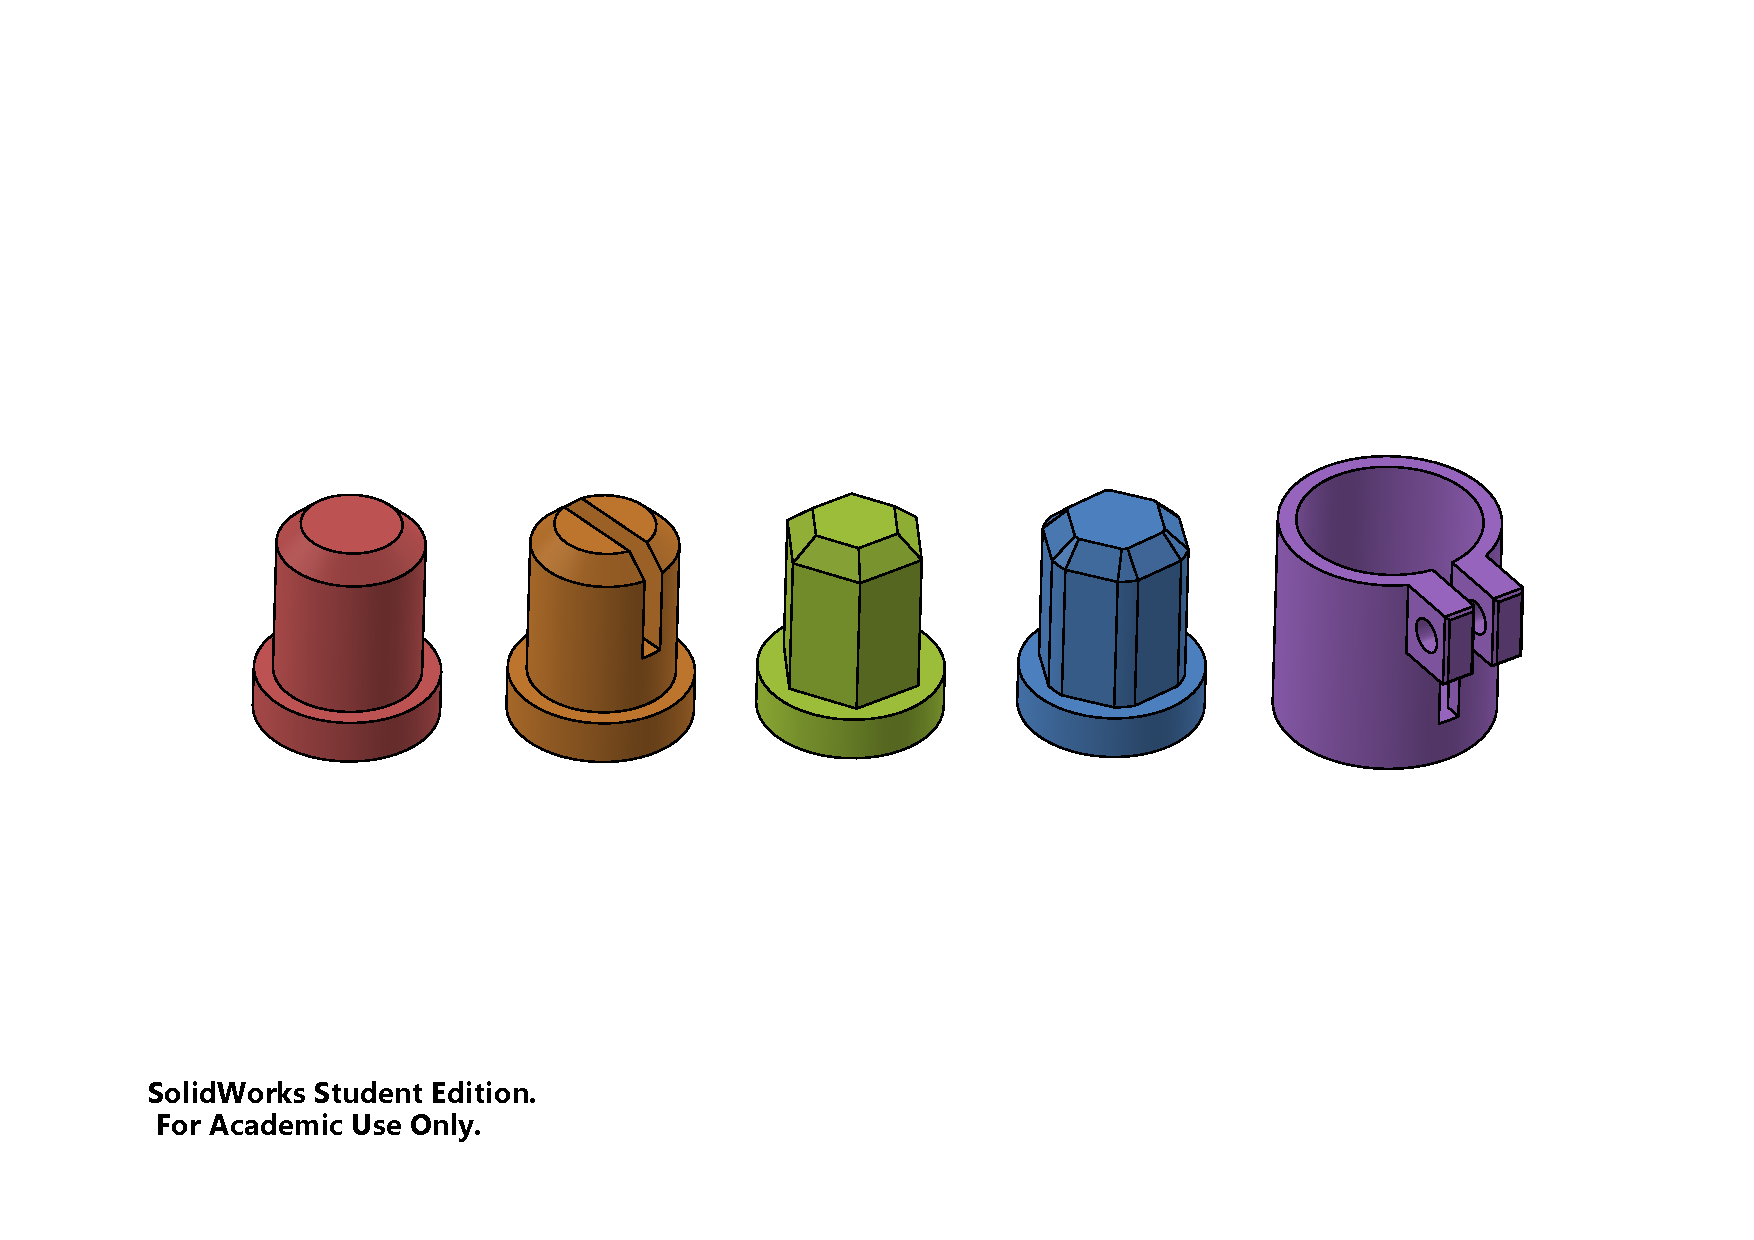
\includegraphics[clip, trim=3cm 6cm 3cm 6cm, width=1\linewidth]{figures/plug-concepts}
        \caption[Render of the plug concepts considered for the attachment of aluminium shafts onto joints and pivots]{Render of the plug concepts considered for the attachment of aluminium shafts onto joints and pivots}
        \label{fig:mechDesign-plugConcepts}
        \end{figure}
        
        % TODO: Label the plugs
        
        The plug that was selected was hexagonal in shape but had edges which were filleted to match the inside surface of the aluminium tube. This was a hybridisation of the cylindrical plug, which introduced a very low window of tolerance in the manufacture of the joints, and the simple hexagonal plug. The filleted edges increased the contact surface area with the inside of the tube, improving the effectiveness of the fit, whilst allowing for greater manufacturing tolerances. In case the plugs proved to be lacking the required strength, a hole could have been drilled down the centre of the plug and a steel rod could be glued into place to strengthen the joint, specifically at the intersection of the middle body and the plug. A nut and bolt were added to the plug-tube assembly as in Figure~\ref{fig:mechDesign-plugTubeBearingDetail} to improve the fitting and prevent rotation of the tube around the axis of the plug.
        
        \begin{figure}[h!]
          \centering
          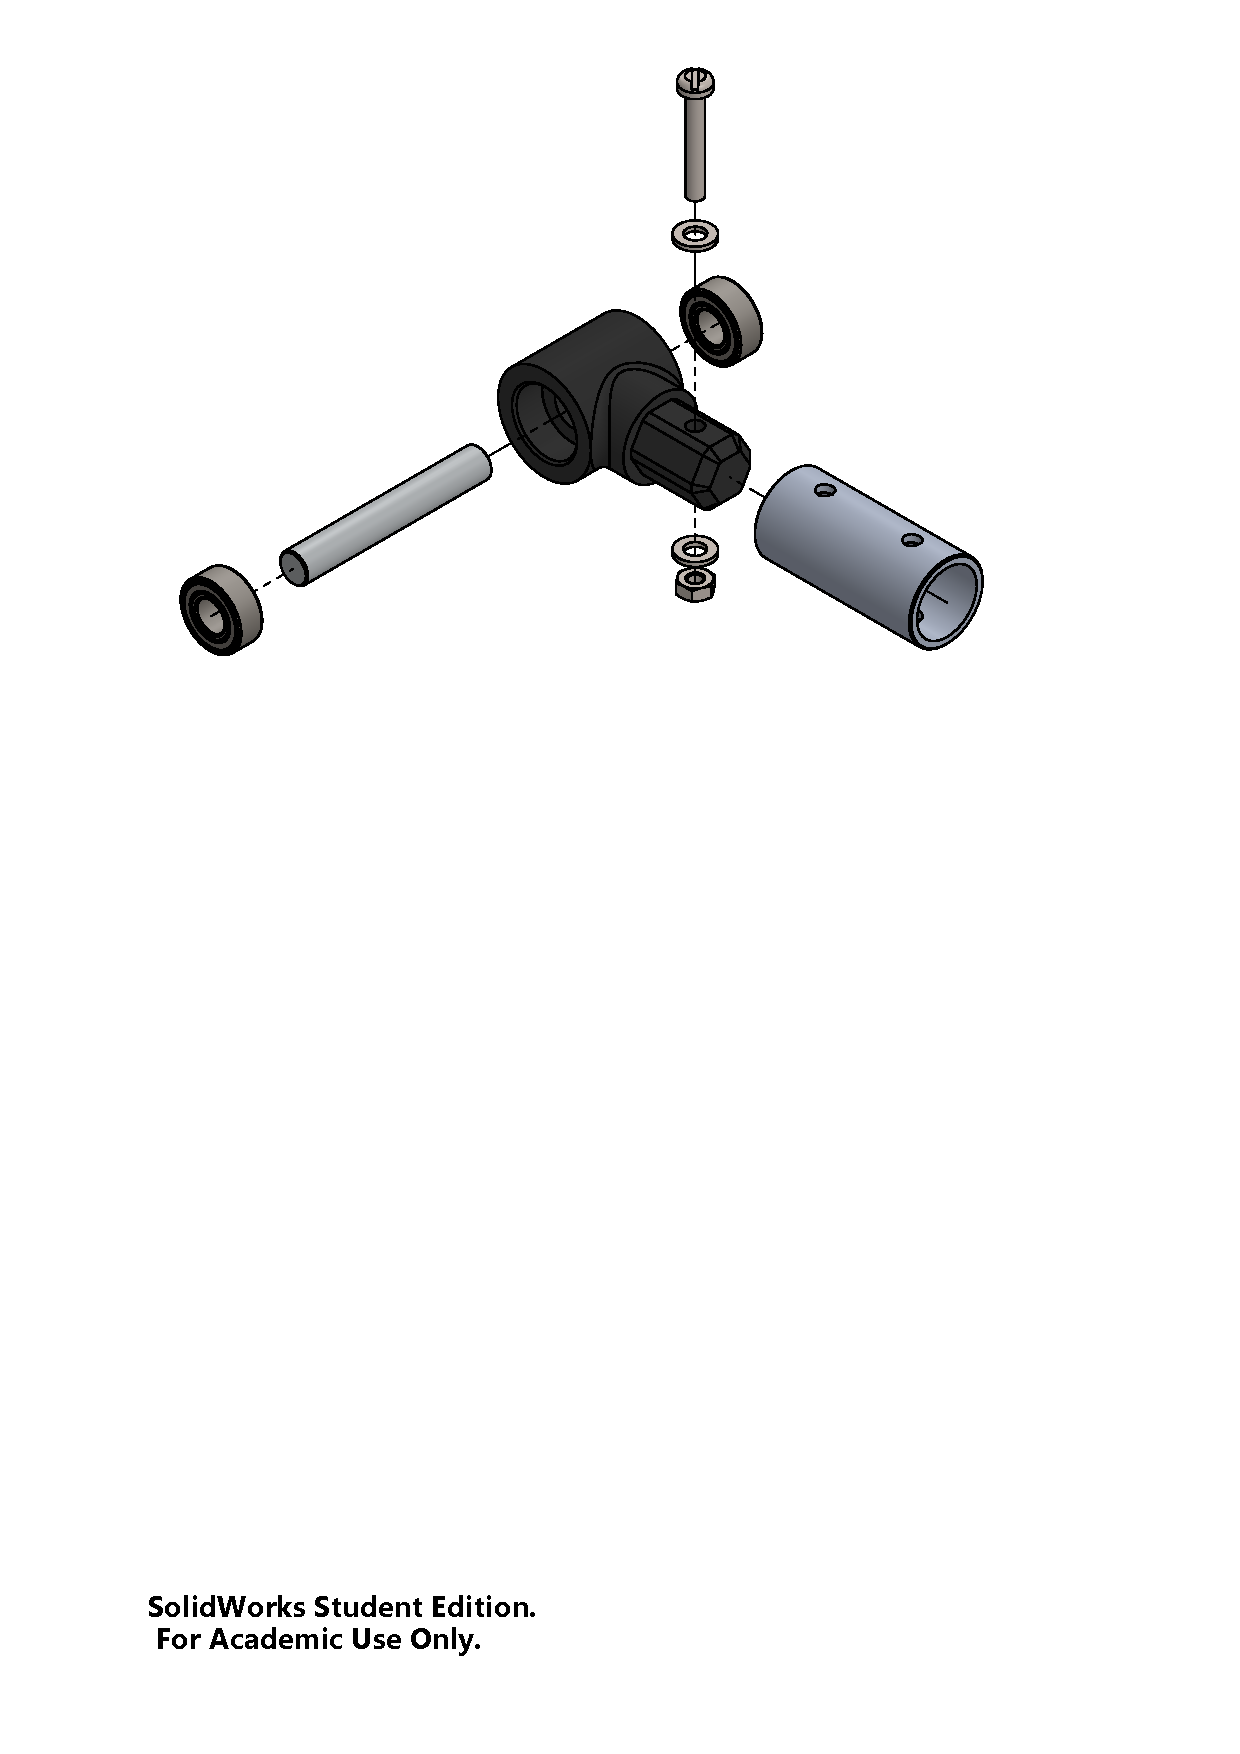
\includegraphics[clip, trim=2cm 17cm 2cm 1cm, width=0.8\linewidth]{figures/plug-tube-bearing}
          \caption[An isometric exploded view of the plug-tube-bearing assembly concept for the suspension system]{An isometric exploded view of the plug-tube-bearing assembly concept for the suspension system}
          \label{fig:mechDesign-plugTubeBearingDetail}
        \end{figure}        
        
        An extension to the rocker joint was made in the form of a ``fin'' feature to allow for the connection of the differential system. The feature was added ``in-place'' in the 3D model after the differential had been added to the assembly so that correct alignment was ensured.
        
        Finally, features for the press-fitting of bearings were added to the joints that required them. Bearings were chosen at this point to be of dimensions shown in Figure~\ref{fig:mechDesign-bearingShaftDetail} in which the shaft diameter is also shown. A single bearing alone was not suitable to provide support against bending torques brought about when the shafts were to be put under load, thus each free-moving joint had two bearings on either extremity. A hole through the centre of the bearing bores of $\diameter8$ mm was included to allow the shafts to extend to the outward-facing bearings. The final designs for each of the three joints are shown in Figures~\ref{fig:mechDesign-rockerJointDetail}, \ref{fig:mechDesign-bogieJointFixedDetail} and \ref{fig:mechDesign-bogieJointFreeDetail}.
        
        \begin{figure}[h!]
          \centering
          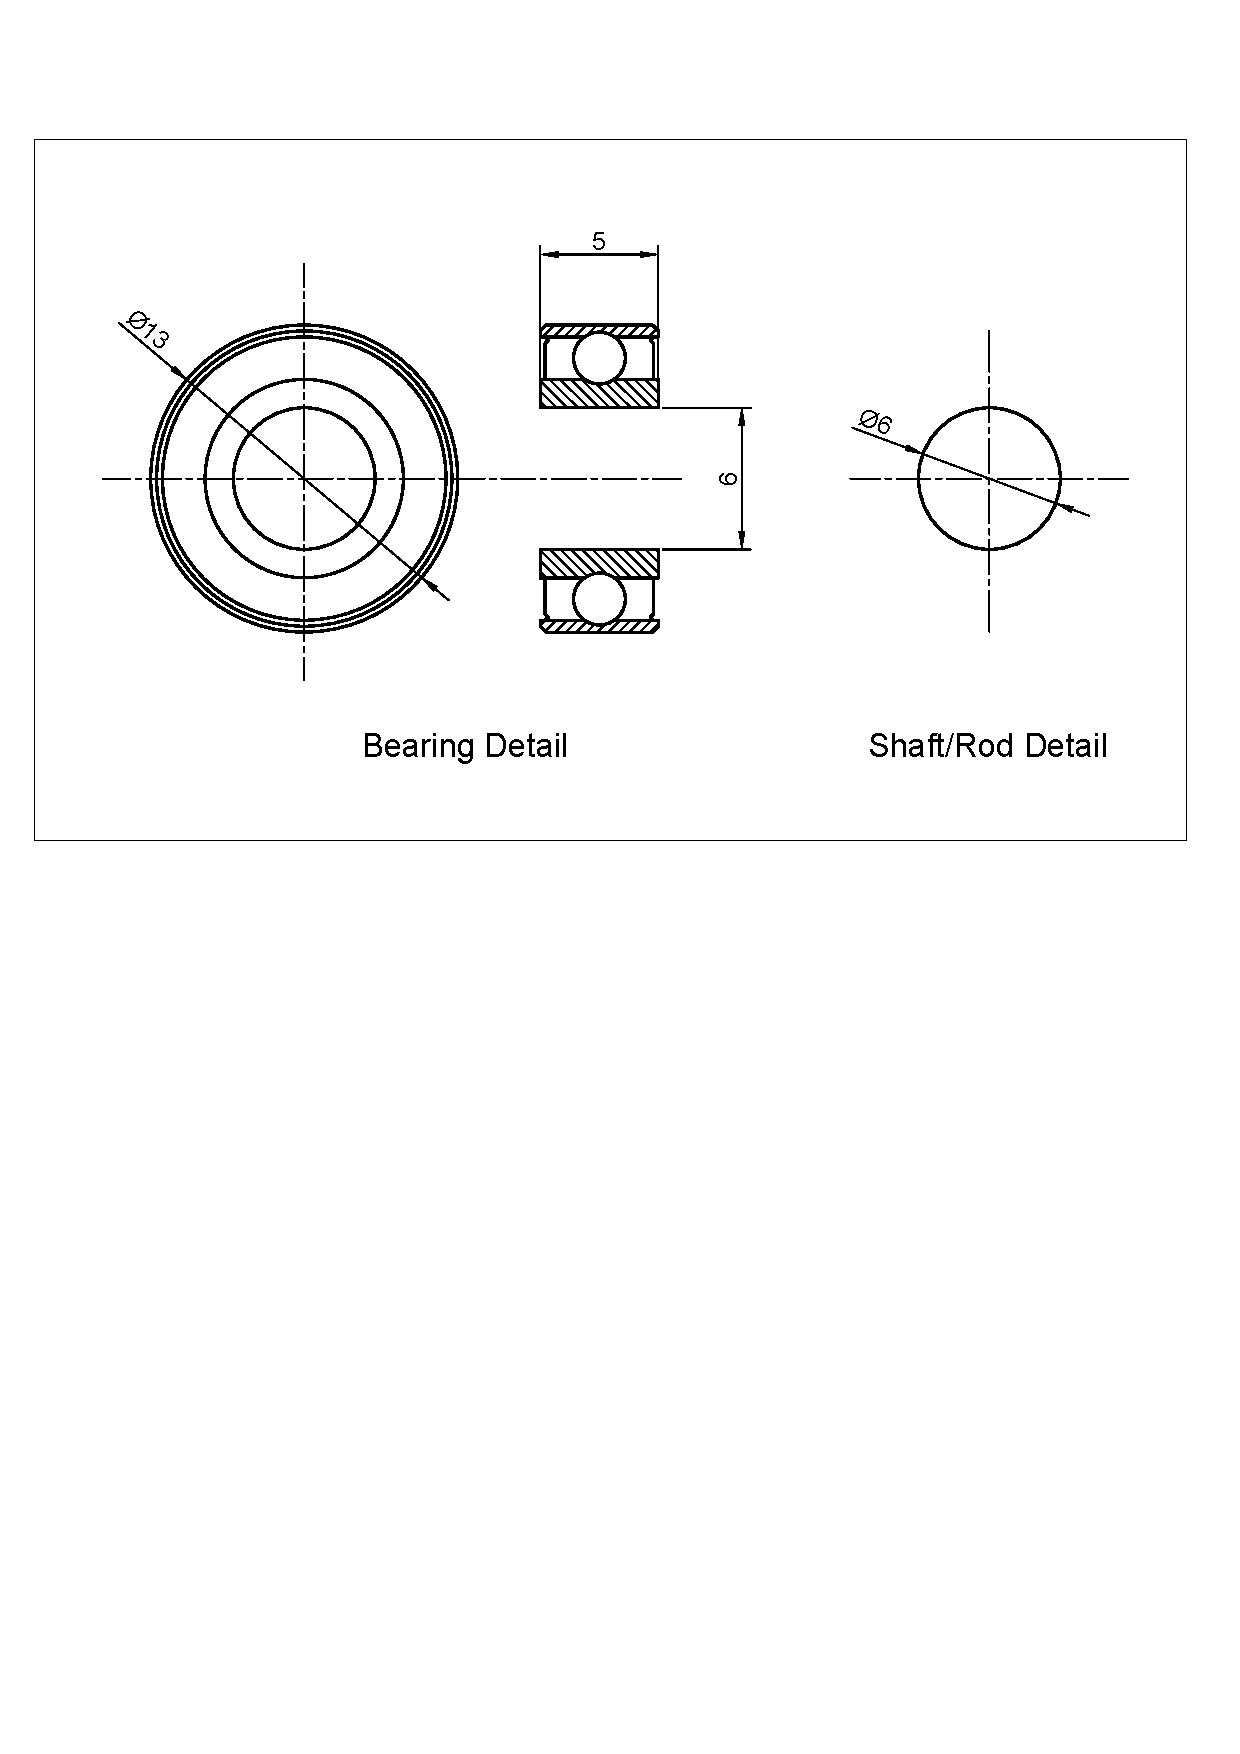
\includegraphics[clip, trim=2cm 16cm 2cm 3cm, width=0.7\linewidth]{figures/bearing-shaft-detail}
          \caption[Detail of the bearings and shaft chosen for all applicable areas]{Detail of the bearings and shaft chosen for all applicable areas}
          \label{fig:mechDesign-bearingShaftDetail}
        \end{figure}        
        
        \begin{figure}[h!]
        \centering
        \subfloat[]{
          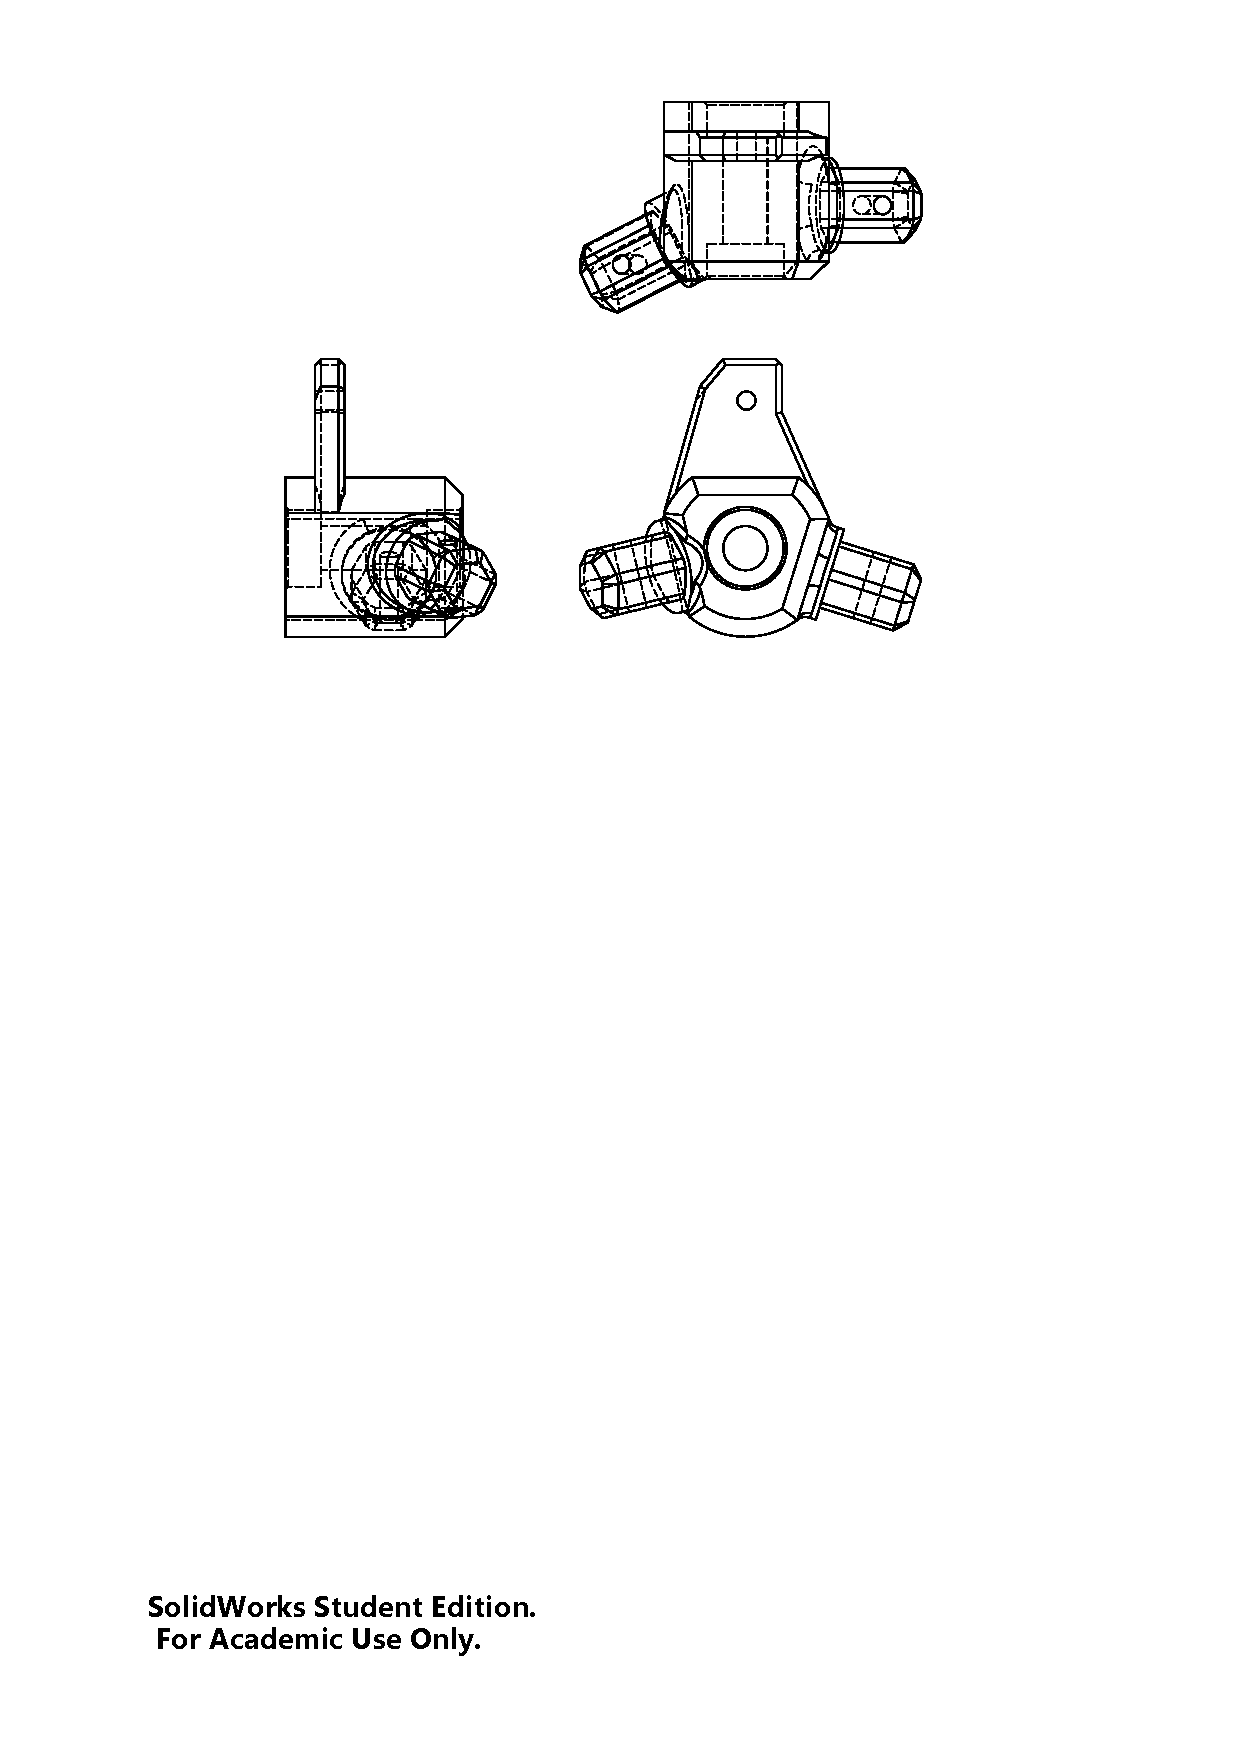
\includegraphics[clip, trim=4cm 18cm 4cm 1cm, width=.59\linewidth]{figures/rocker-joint.PDF}
        }
        \subfloat[]{
          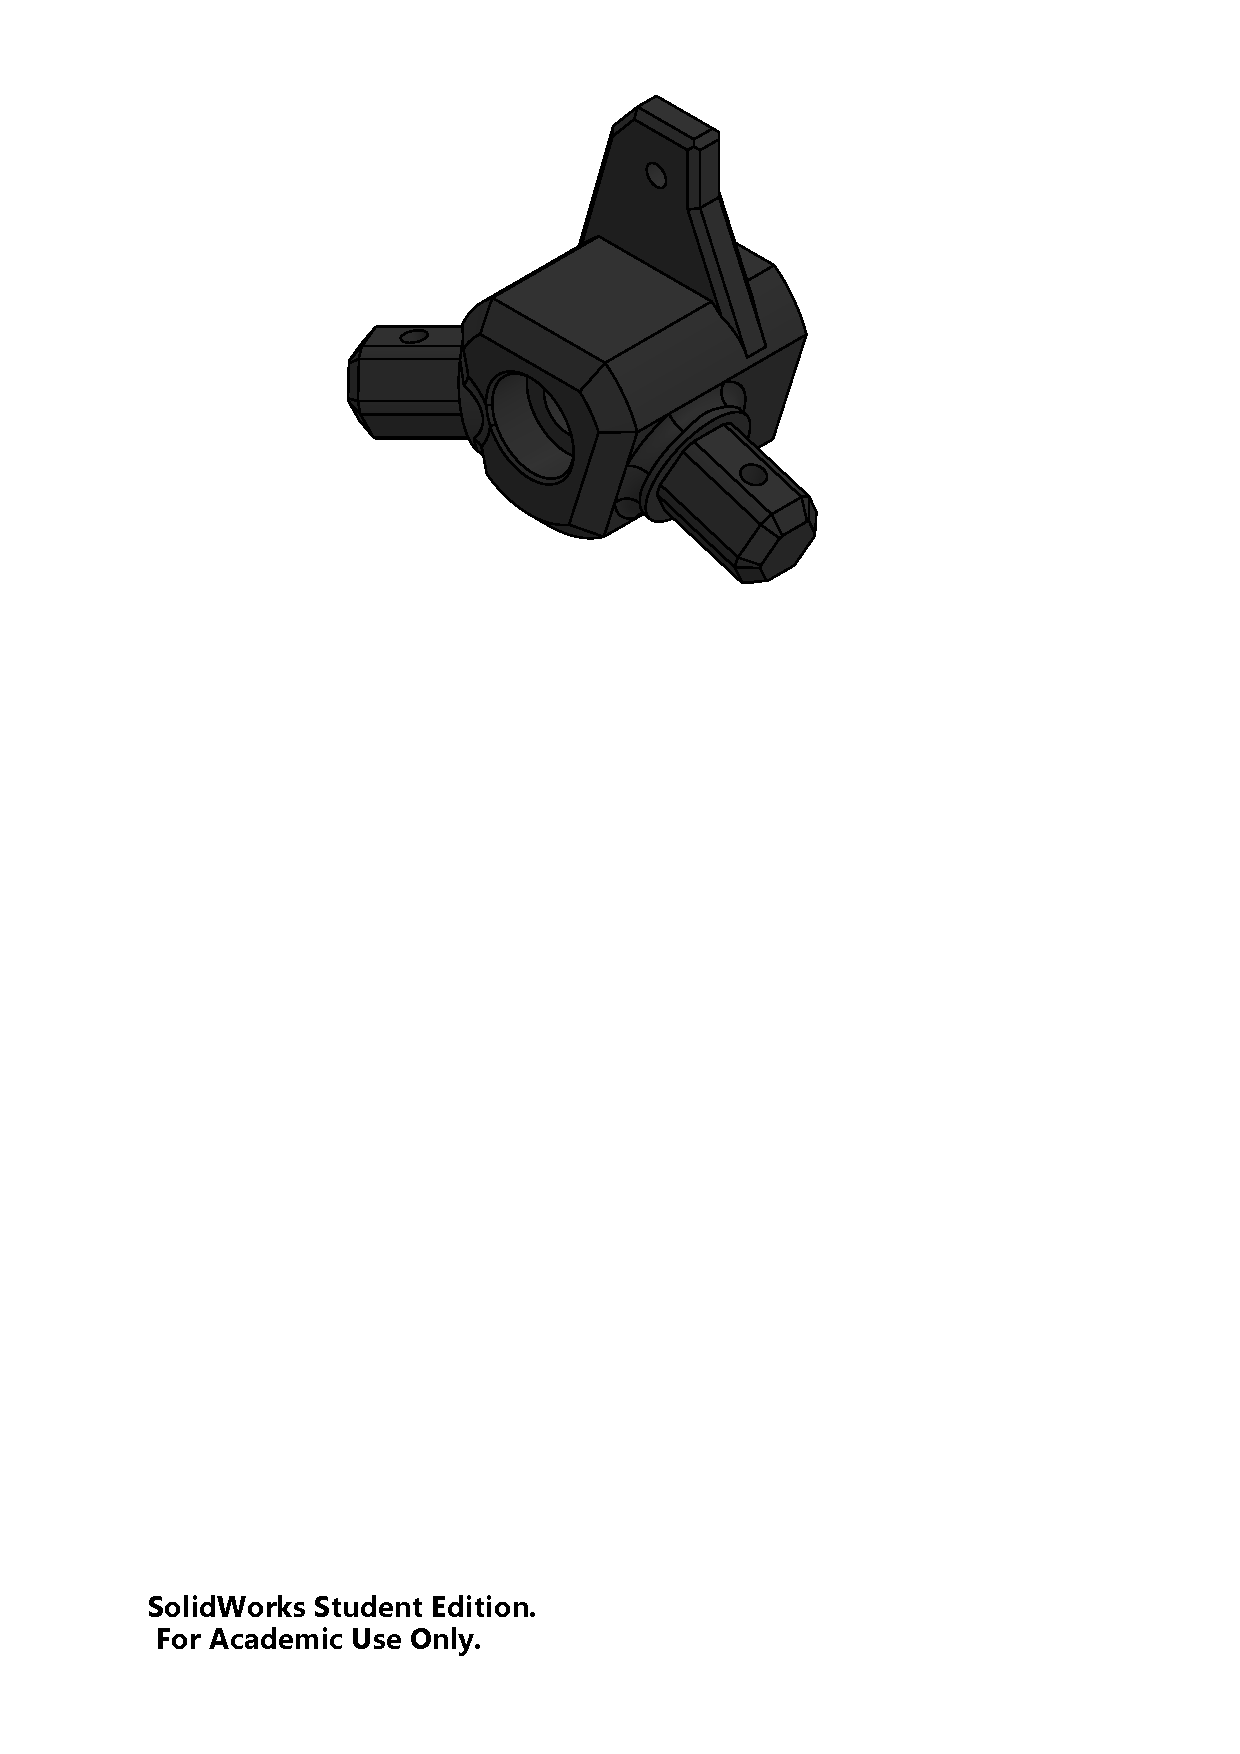
\includegraphics[clip, trim=6cm 18cm 6cm 1cm, width=.4\linewidth]{figures/rocker-joint-iso.PDF}
        }
        \caption[Detailed drawings of the rocker joint component for one side of the suspension system]{Detailed drawings of the rocker joint component for one side of the suspension system}
        \label{fig:mechDesign-rockerJointDetail}
        \end{figure}
        
        \begin{figure}[h!]
        \centering
        \subfloat[]{
          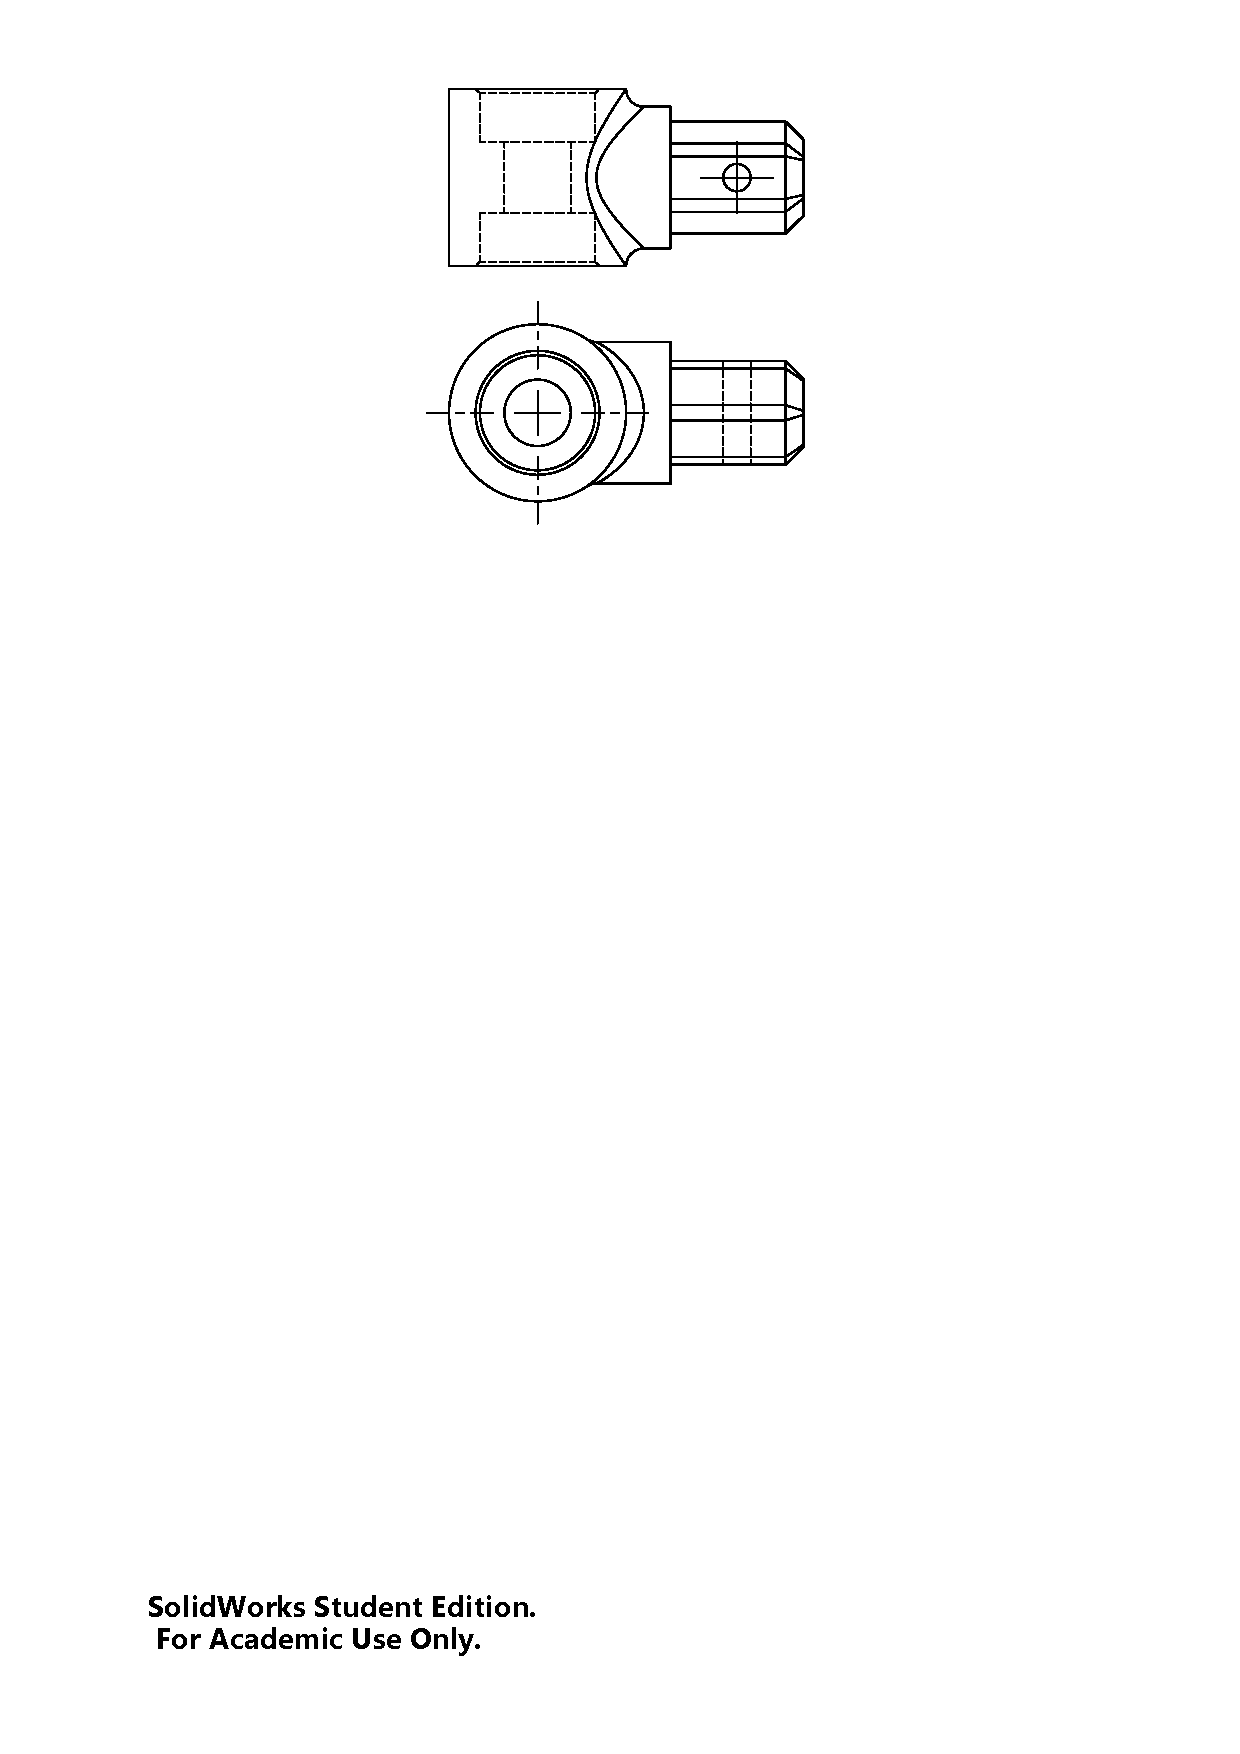
\includegraphics[clip, trim=6cm 18cm 6cm 1cm, width=.45\linewidth]{figures/bogie-joint-free.PDF}
        }
        \subfloat[]{
          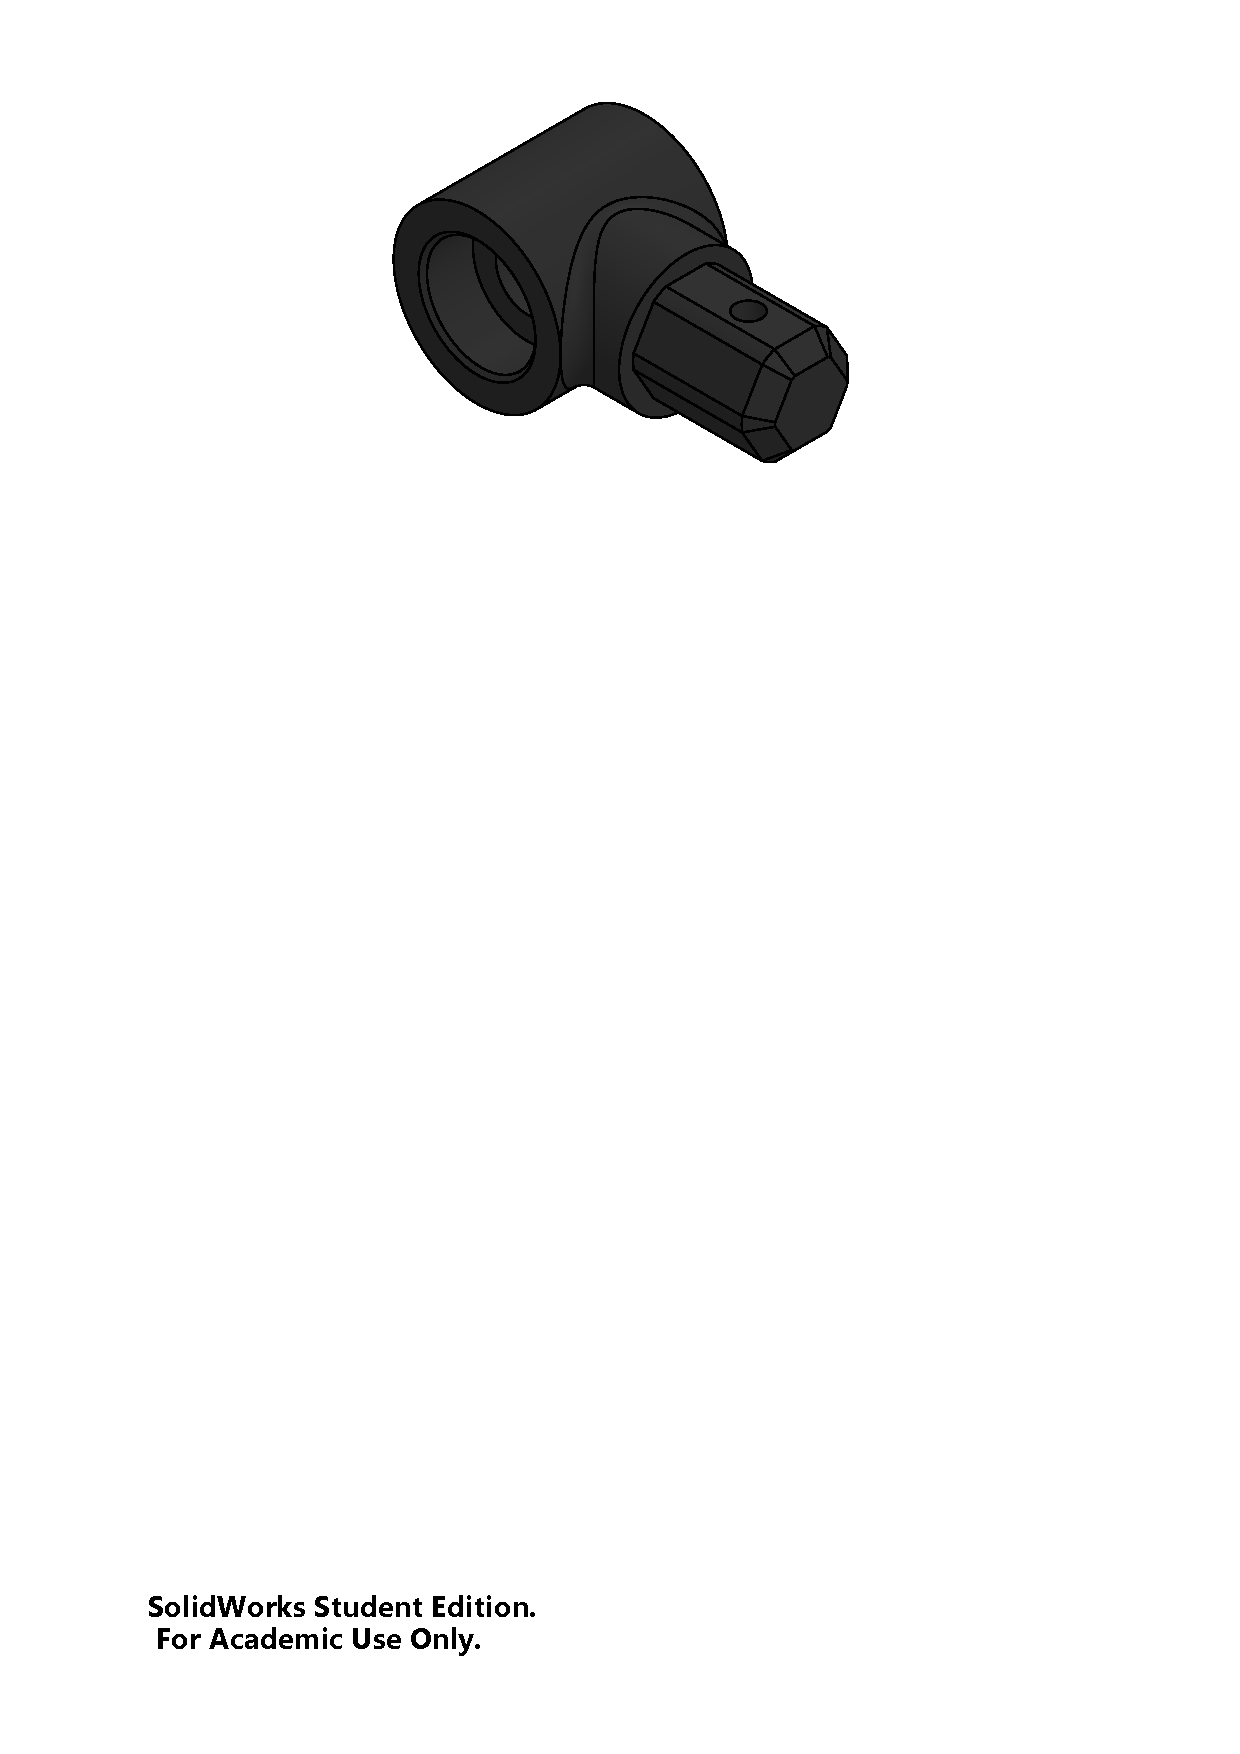
\includegraphics[clip, trim=6cm 18cm 6cm 1cm, width=.45\linewidth]{figures/bogie-joint-free-iso.PDF}
        }
        \caption[Detailed drawings of the free bogie joint component for one side of the suspension system]{Detailed drawings of the free bogie joint component for one side of the suspension system}
        \label{fig:mechDesign-bogieJointFreeDetail}
        \end{figure}
        
        \begin{figure}[h!]
        \centering
        \subfloat[]{
          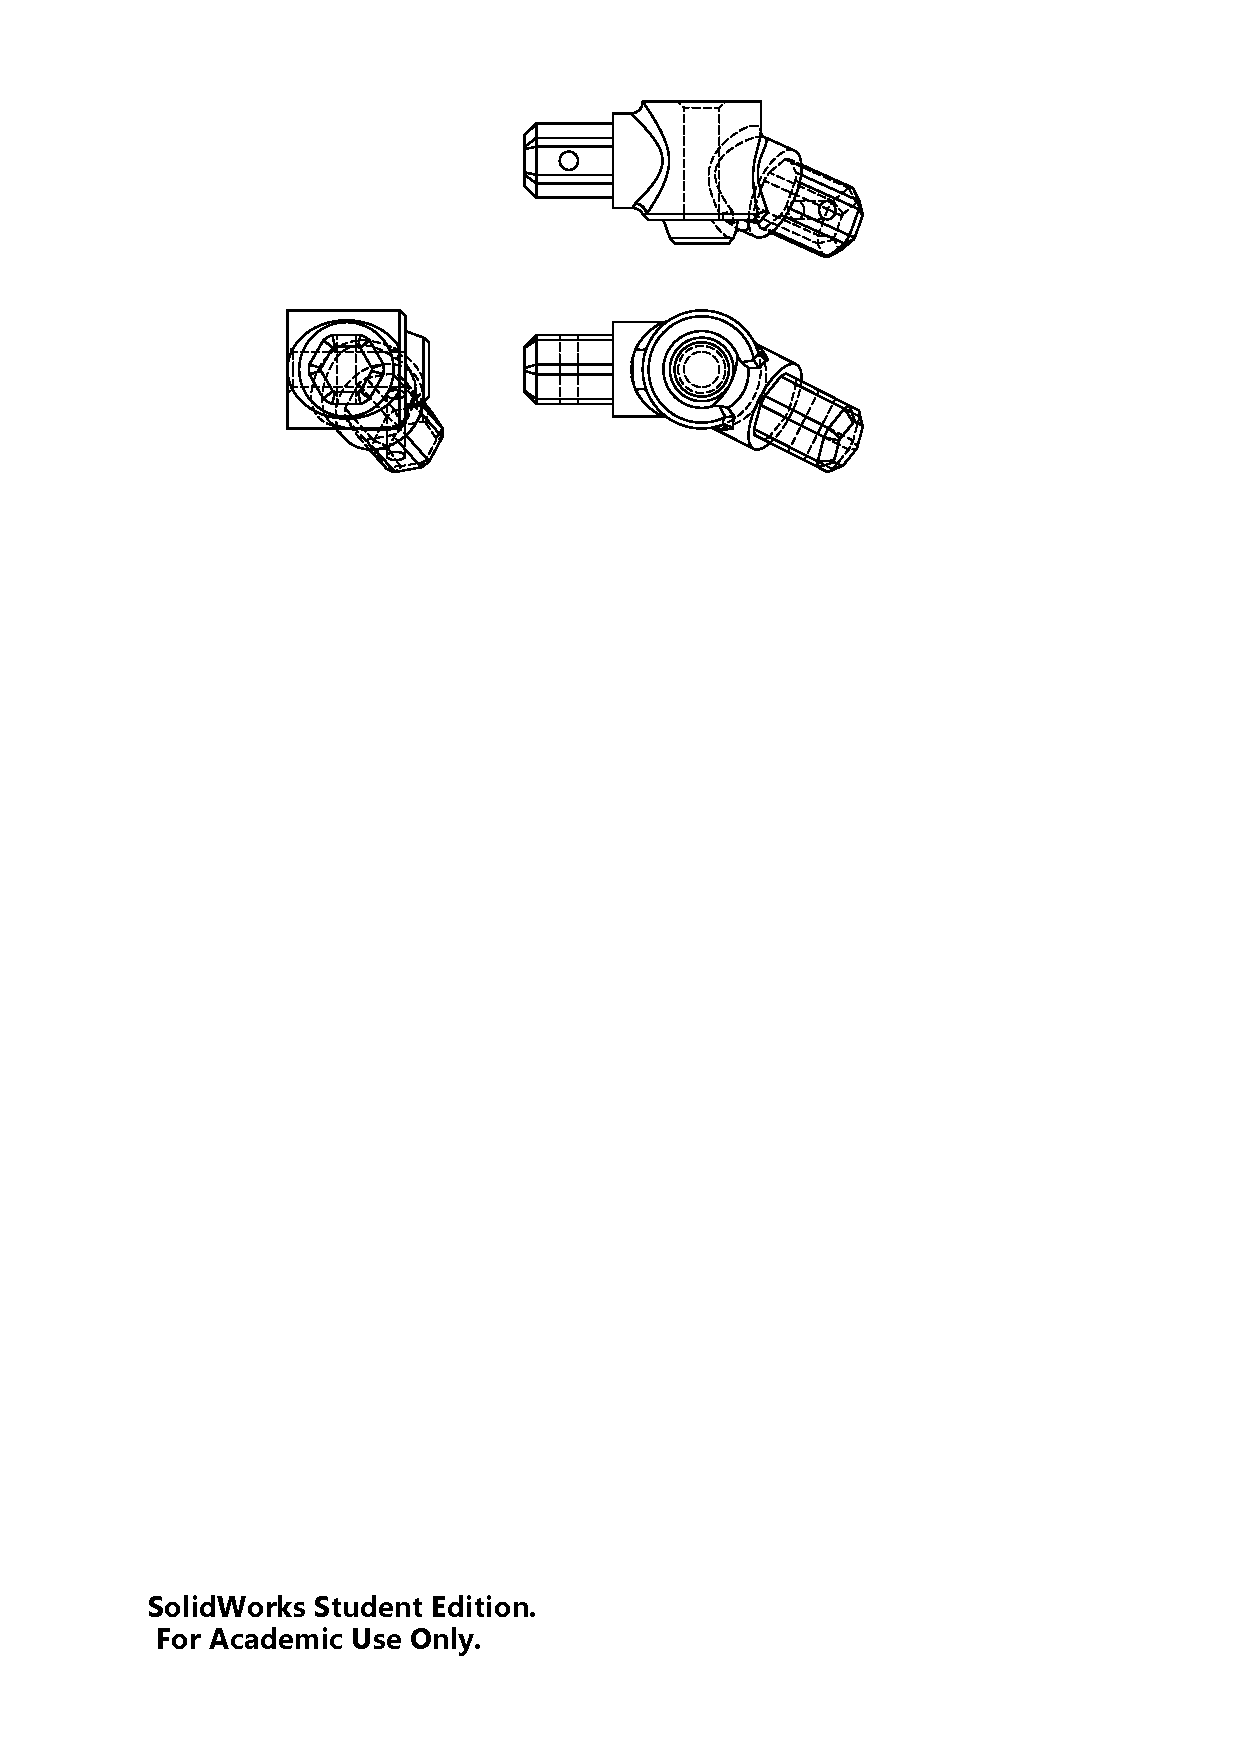
\includegraphics[clip, trim=4cm 20cm 4cm 1cm, width=.65\linewidth]{figures/bogie-joint-fixed.PDF}
        }
        \subfloat[]{
          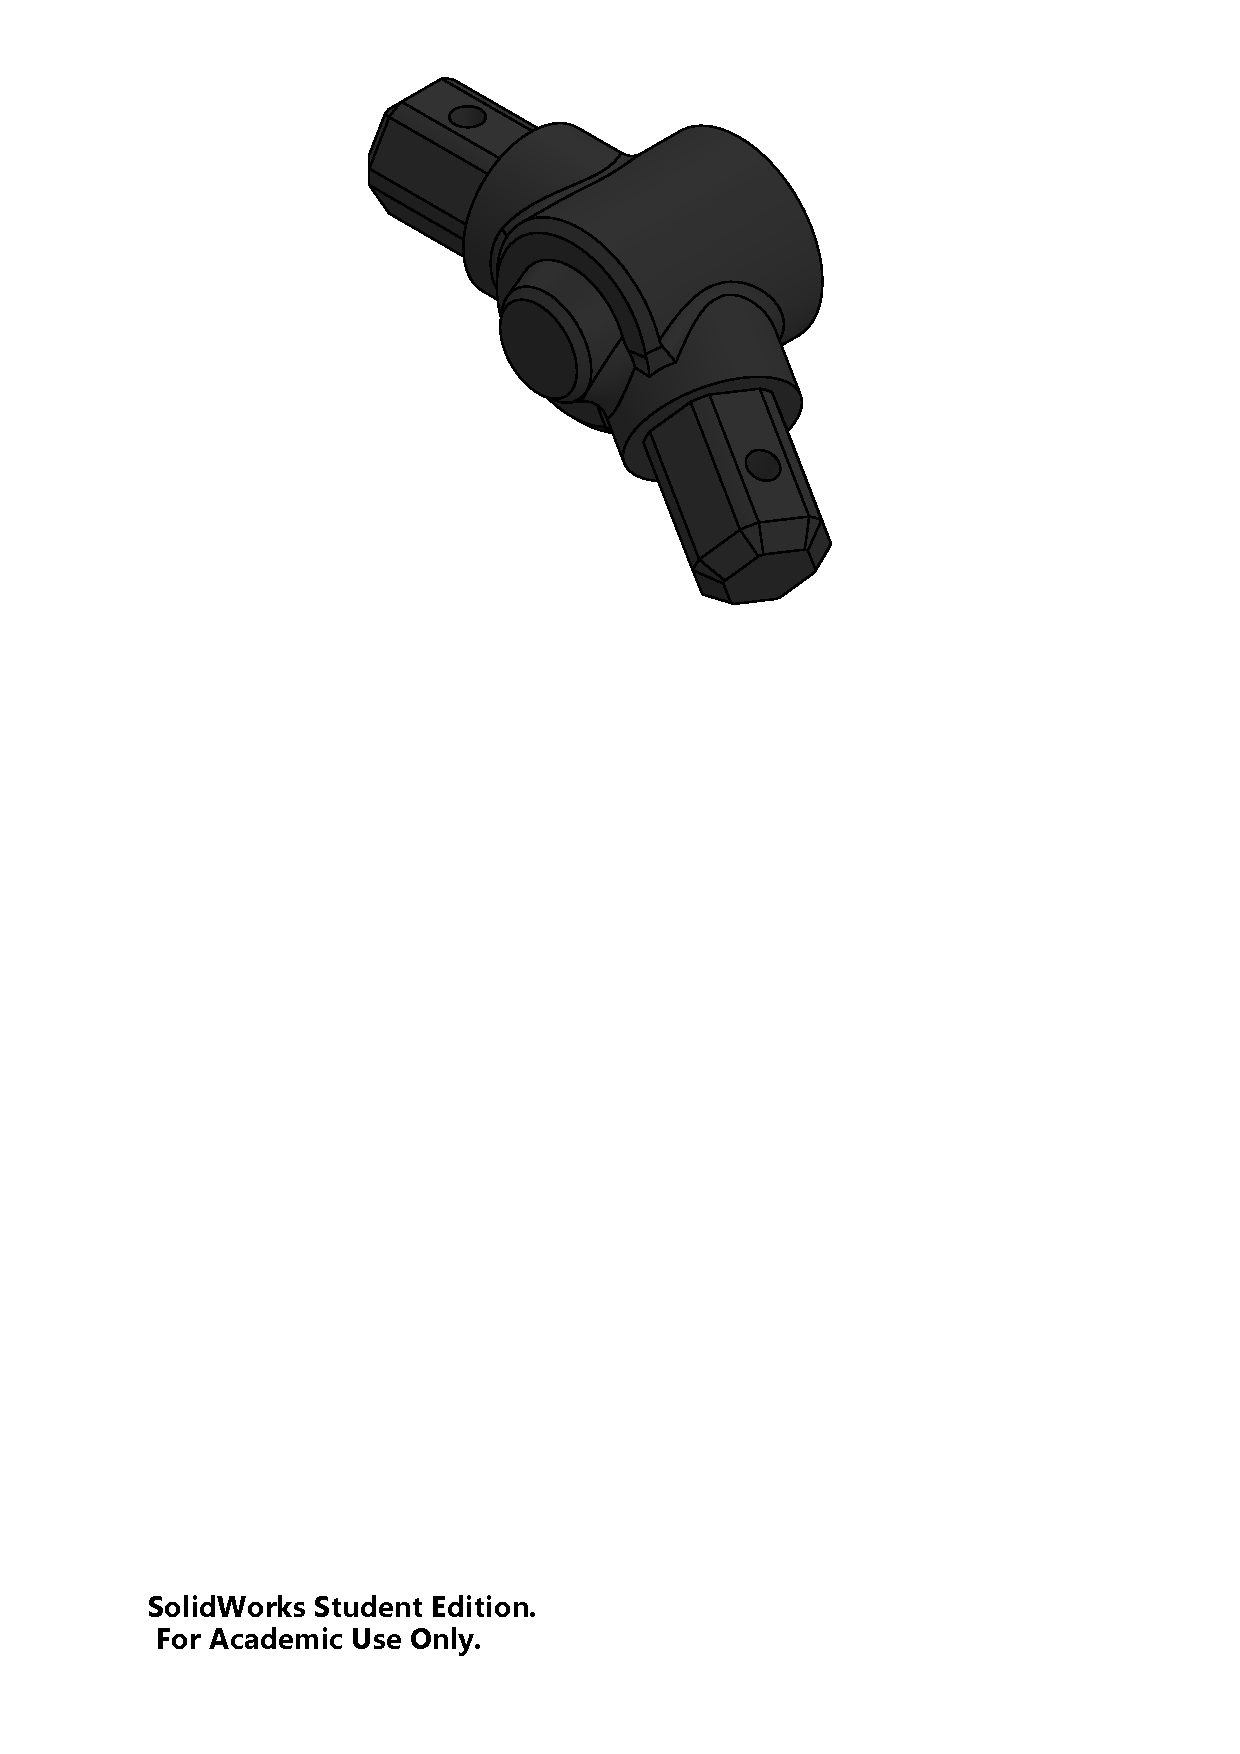
\includegraphics[clip, trim=6cm 18cm 6cm 1cm, width=.34\linewidth]{figures/bogie-joint-fixed-iso.PDF}
        }
        \caption[Detailed drawings of the fixed bogie joint component for one side of the suspension system]{Detailed drawings of the fixed bogie joint component for one side of the suspension system}
        \label{fig:mechDesign-bogieJointFixedDetail}
        \end{figure}
        
      \subheading{Wheels}\\\\
        Six wheels were to be designed, four of which were driven by the sub-micro servos (front and rear wheels) and the two centre wheels were to be mounted onto fixed shafts with bearings. All six of the wheels on the real \textit{Curiosity} are actuated to ensure robustness of the driving mechanisms in a wider range of terrain types and traversal situations. It is also a feature of redundancy in that if one of the motors fails, the rover is capable of continuing operation. However, it was decided that for this model only the front and rear wheels would be actuated given the reduced power to weight ratio compared to that of \textit{Curiosity}. Redundancy was not an issue worth the resultant extra servos and the incurred additional control complexity.
        
        As mentioned in Section~\ref{subsec:rover-concept-proposals}, the wheels were a great opportunity to make use of the aesthetic accuracy of additive manufacturing thus the wheel was modelled so as to replicate the cross-sectional curve of the outer shell of the wheel. Included were the tread patterns for traction as well as the morse-code emboss which read ``JPL'', used on \textit{Curiosity} to acquire optical estimates of the distance travelled by the rover. Spokes and a centre cylindrical core was added to the inside of the outer shell, keeping the wheel as a single piece.
        
        The sub-micro servos were accompanied by servo horns that fitted onto the shaft of the servo. The horns were cross-shaped, a layout of which was taken advantage to provide support in the cross-axis plane. The horns were measured and holes were added to the four wheels concerned so that they could be mounted directly to the driving servos. The need for bearings on this assembly was countered by an estimate of the forces developed due to the rover's weight and it was determined that the servos would be capable of taking the estimated load without damage or wear. This also provisioned for easy replacement of wheels and or servos should one of them be damaged.
        
        The same bearing bores and centre hole as on the joint components was added to the cylindrical core of the centre wheels for mounting to the aluminium shafts. The press-fitting of bearings into the wheels was to be of the same nature as that of the joints. Figures~\ref{fig:mechDesign-outerWheelDetail} and \ref{fig:mechDesign-midWheelDetail} show the outer and centre wheel details.
        
        \begin{figure}[h!]
        \centering
        \subfloat[]{
          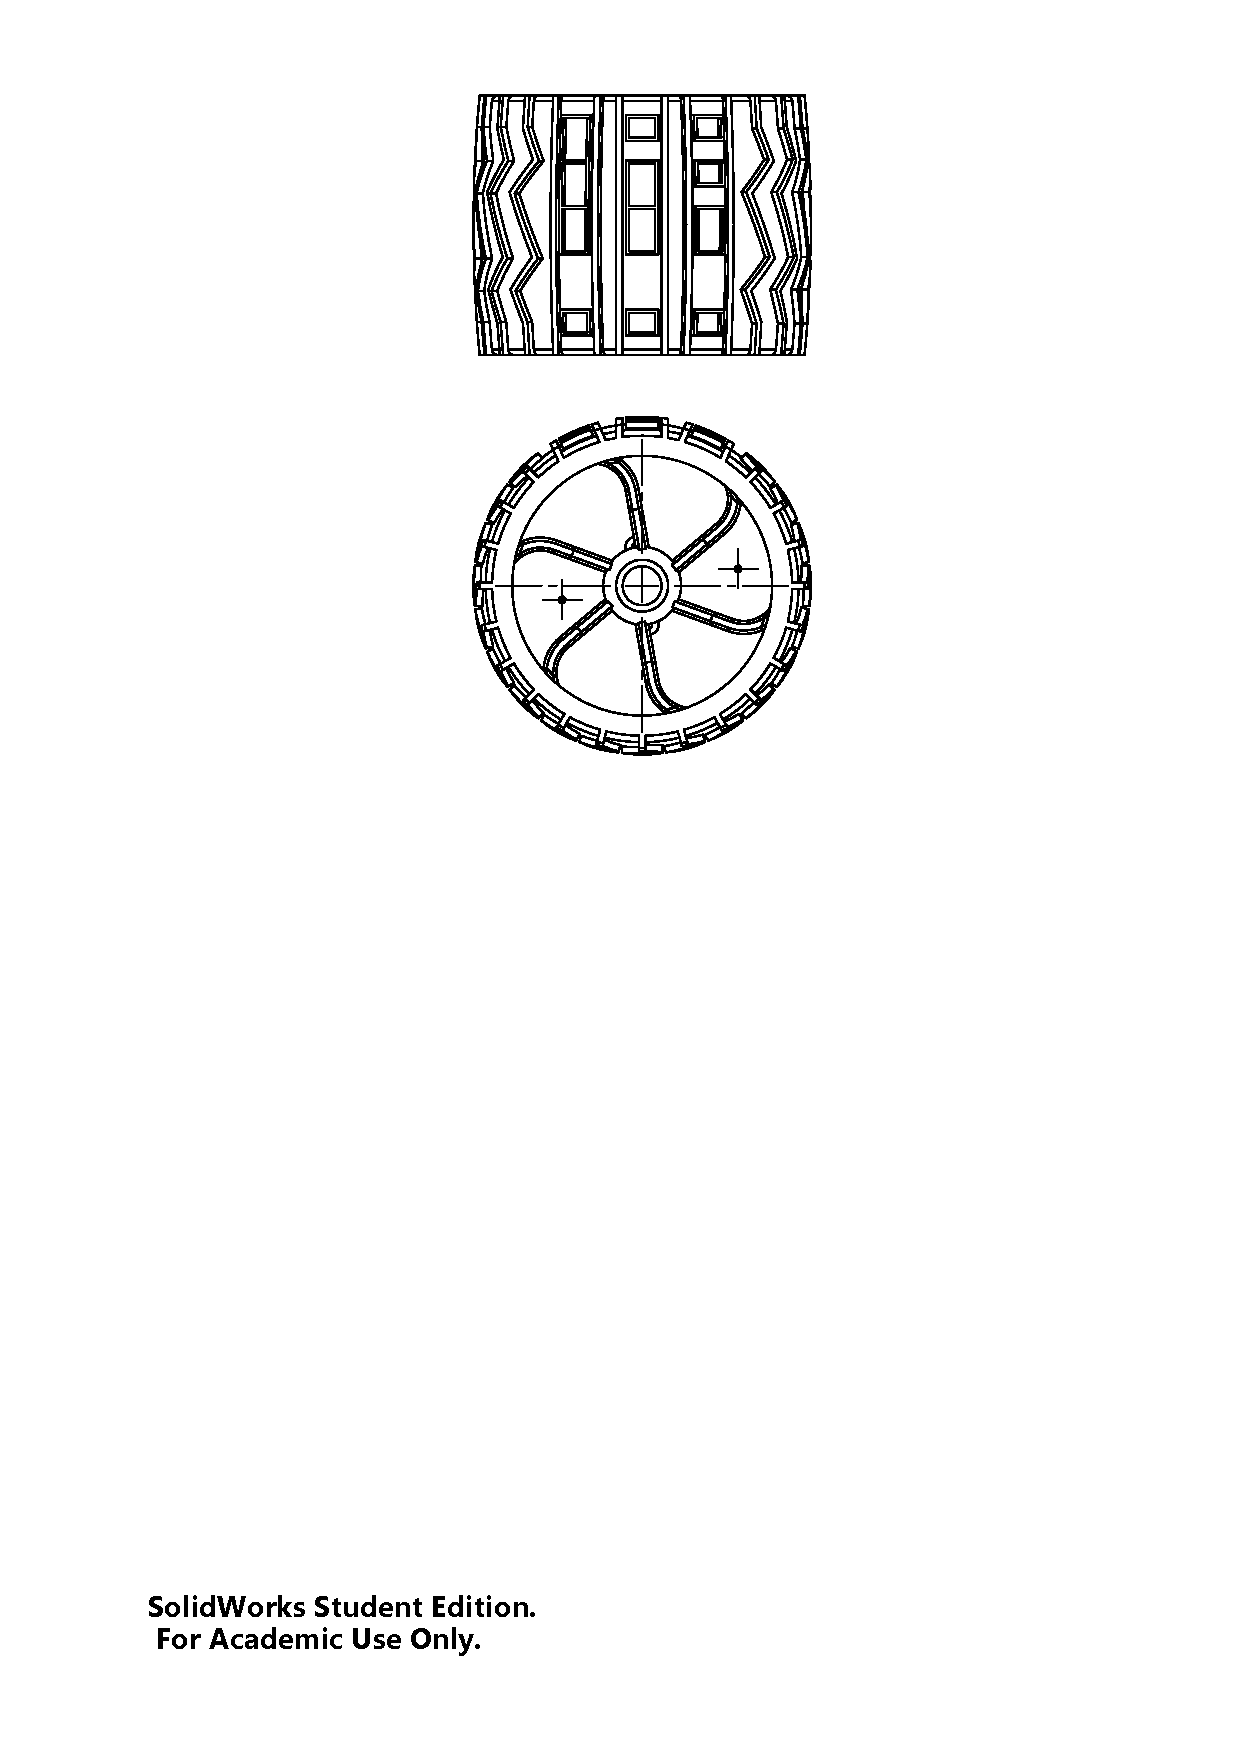
\includegraphics[clip, trim=6cm 16cm 6cm 1cm, width=.5\linewidth]{figures/tire-outer}
        }
        \qquad
        \subfloat[]{
          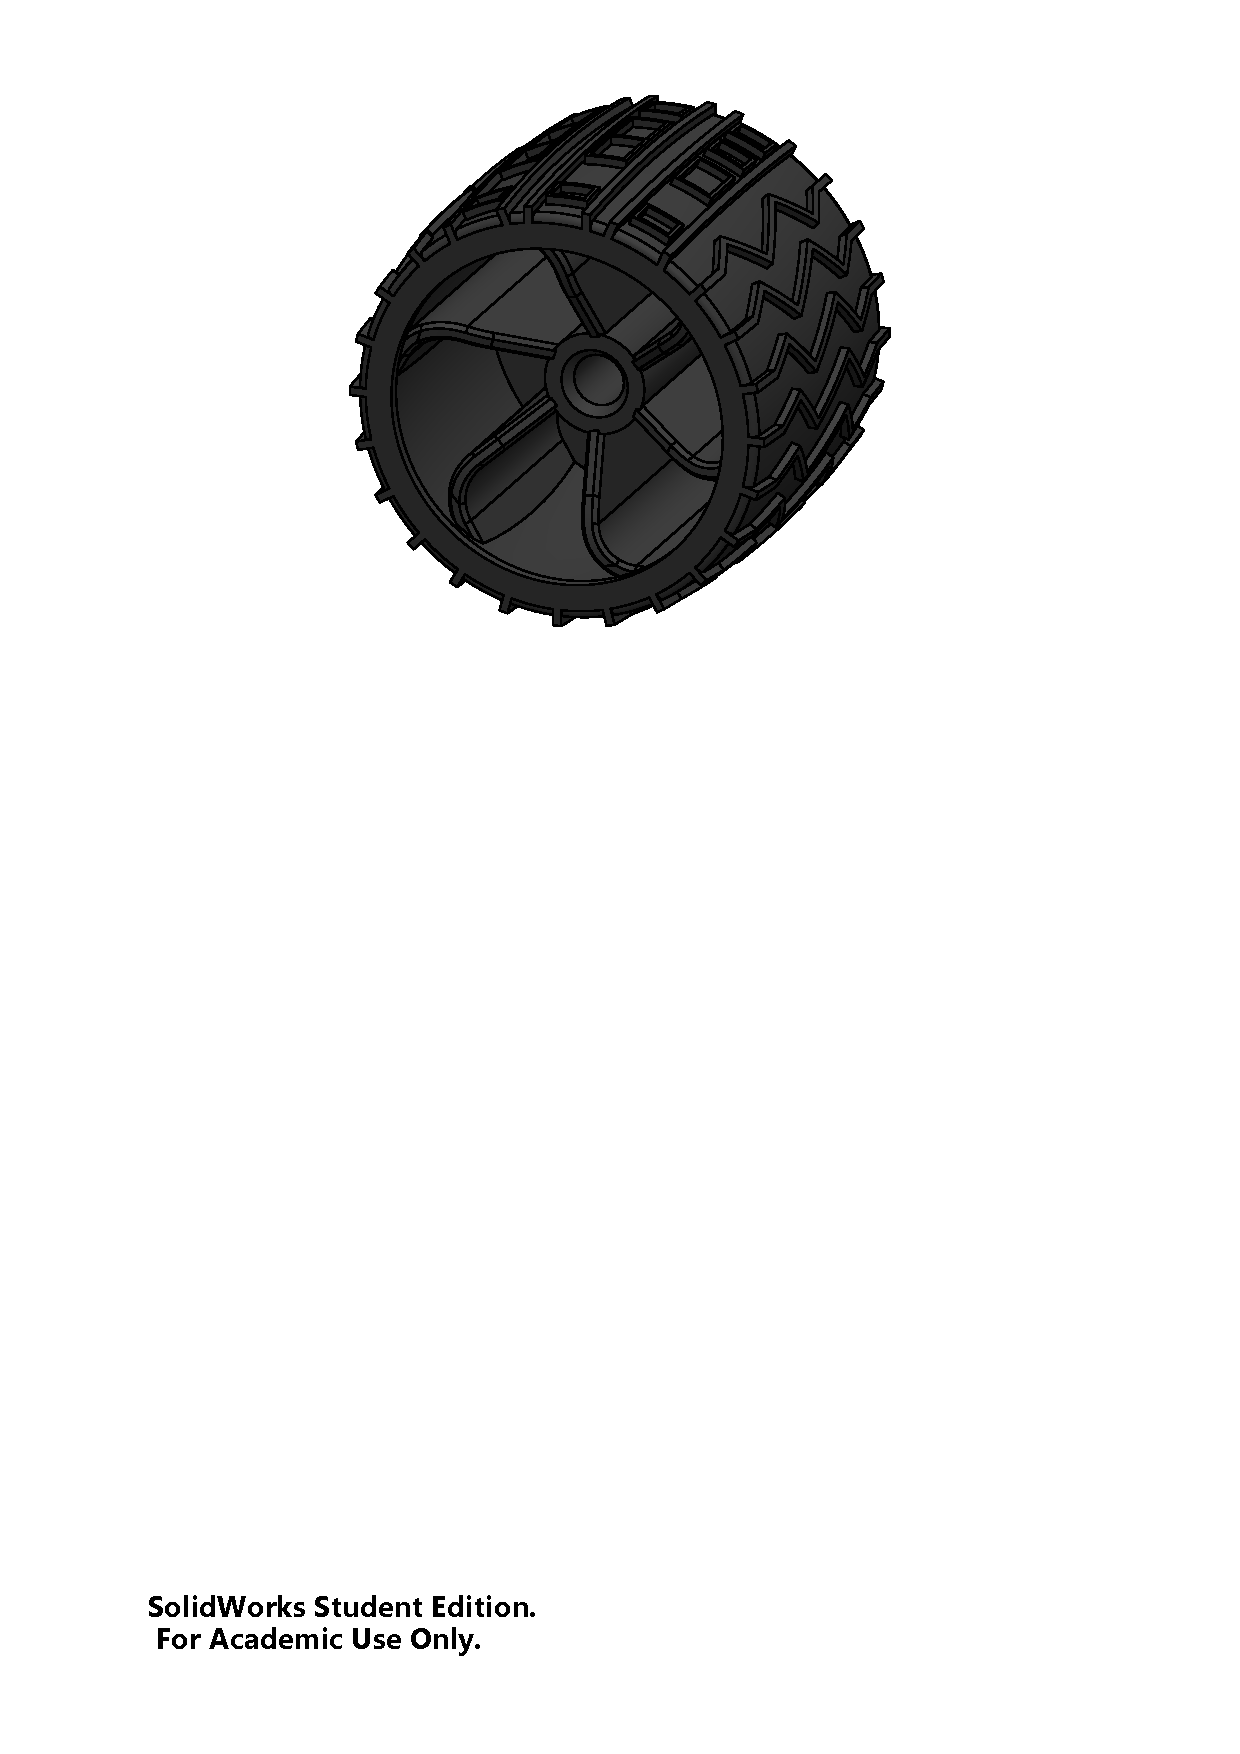
\includegraphics[clip, trim=6cm 16cm 6cm 1cm, width=.4\linewidth]{figures/tire-outer-dimet}
        }
        \caption[Detailed drawings of the leading and trailing wheels]{Detailed drawings of the leading and trailing wheels}
        \label{fig:mechDesign-outerWheelDetail}
        \end{figure}
        
        \begin{figure}[h!]
        \centering
        \subfloat[]{
          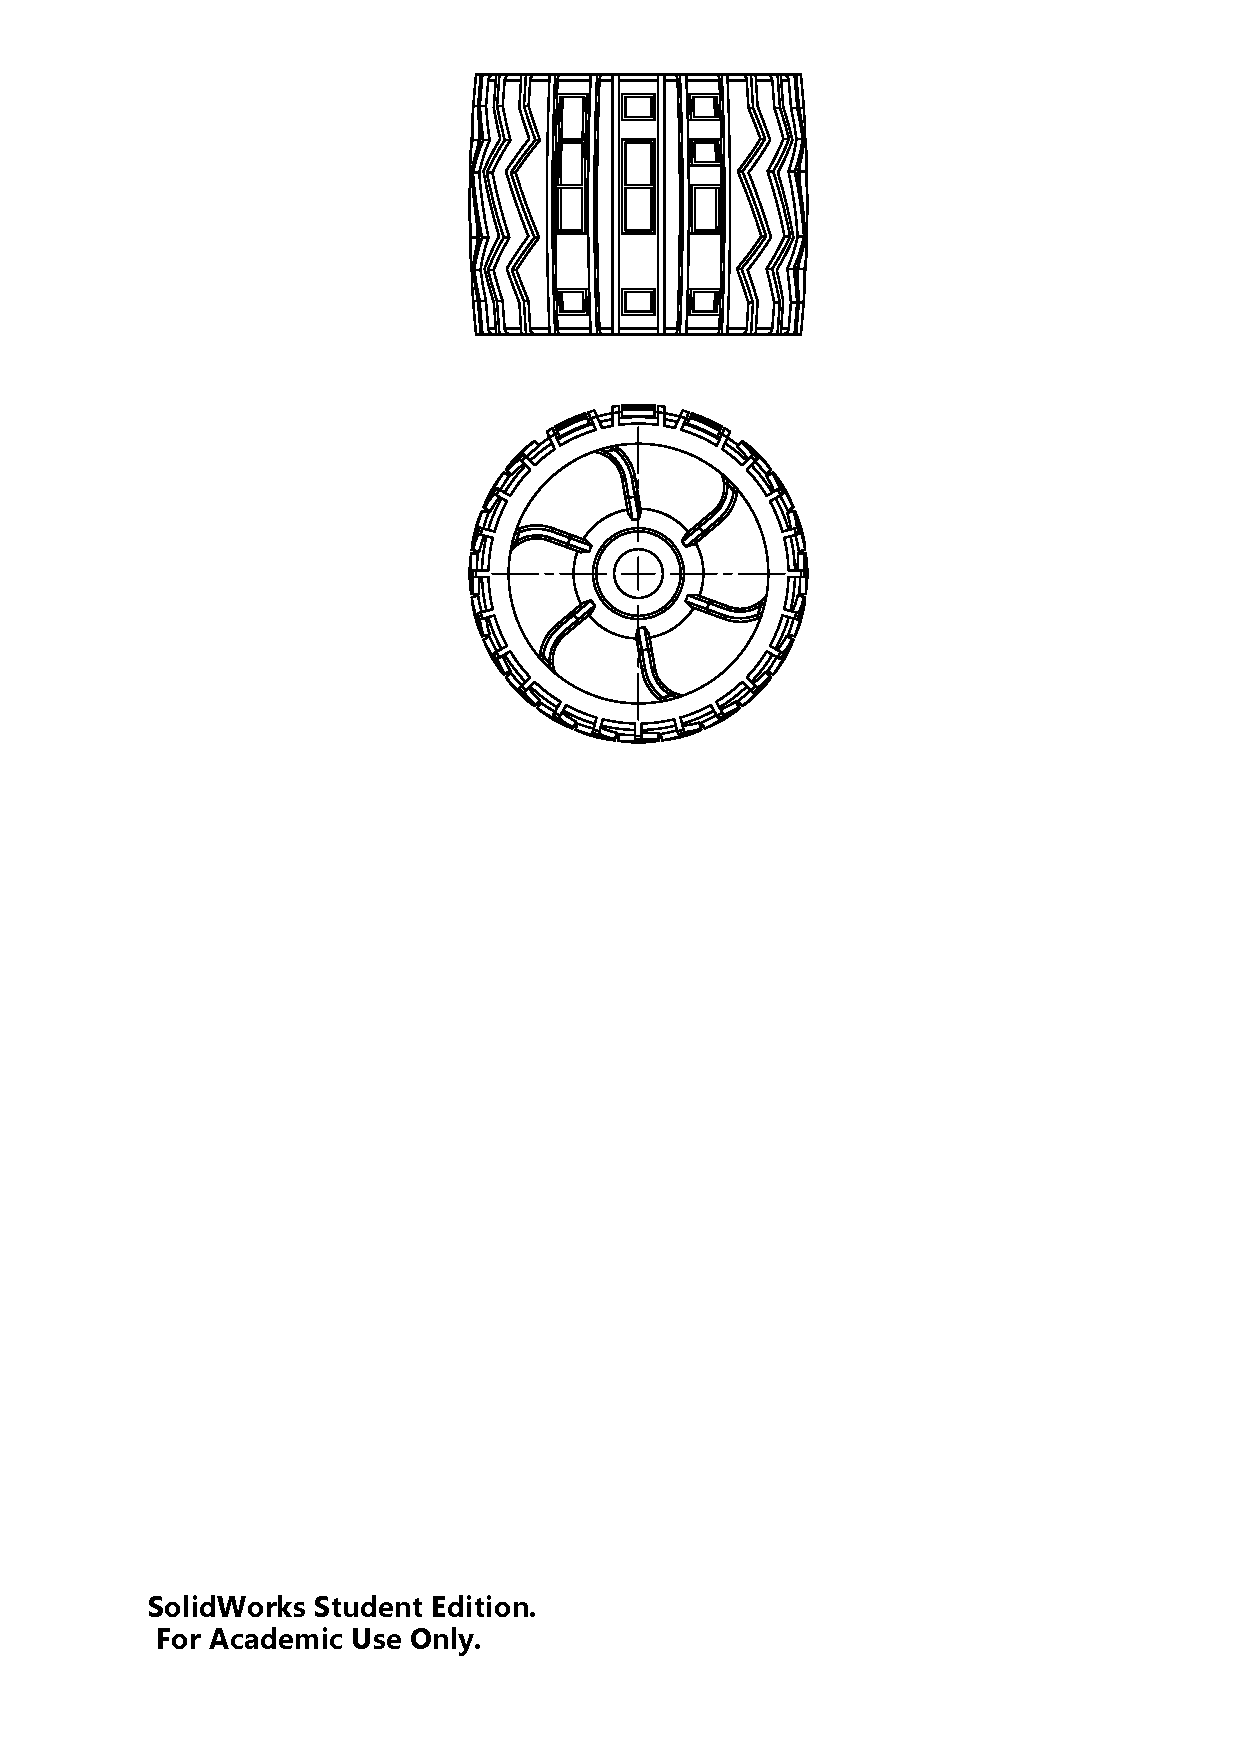
\includegraphics[clip, trim=6cm 16cm 6cm 1cm, width=.5\linewidth]{figures/tire-mid}
        }
        \qquad
        \subfloat[]{
          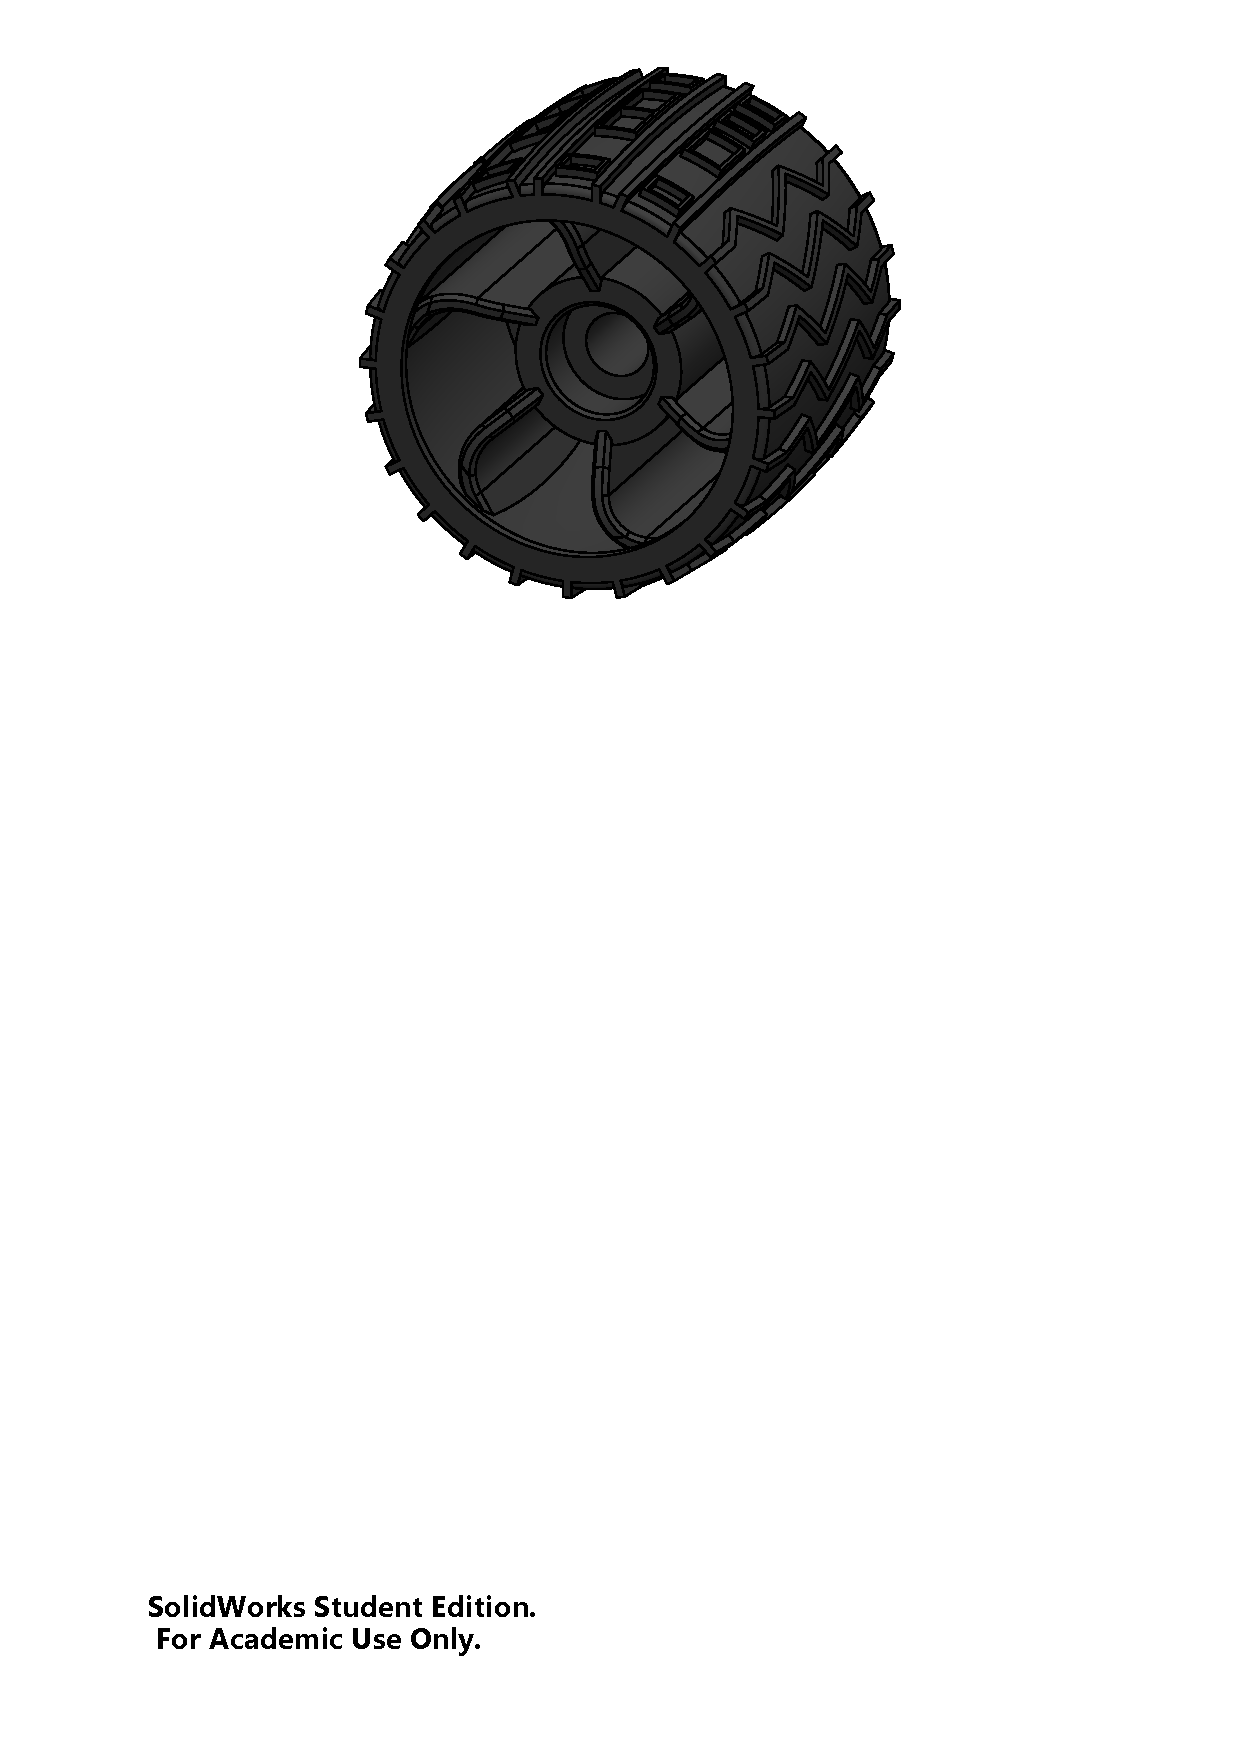
\includegraphics[clip, trim=6cm 16cm 5cm 1cm, width=.4\linewidth]{figures/tire-mid-dimet}
        }
        \caption[Detailed drawings of the centre wheels]{Detailed drawings of the centre wheels}
        \label{fig:mechDesign-midWheelDetail}
        \end{figure}
          
      \subheading{Pivots}\\\\
        Turning the wheel-strut assembly involved the pivot component which had to allow for mounting of a sub-micro steering servo and for attachment to the ends of the fore rocker-tubes and aft bogie-tubes. The same concept for attaching to the aluminium tube as in the case of the joints was applied to the pivots. Thus the design consisted of a L-shaped extrusion with the plug extending from one of the outside flat surfaces. The other surface had a rectangular cut-out the size of the servo body, mounting holes for the servo and ribs for supporting the L-shaped extrusion. Figure~\ref{fig:mechDesign-wheelPivotDetail} shows the pivot component detail for the front wheel assembly.
        
        The front and rear pivots differed slightly due to the different angle of entry of the rocker and bogie tubes towards the centre-points of the wheel assembly. Managing the differences in these angles was aided by use of the 3D skeleton sketch. Again, the front and rear pivots from the left-hand side were mirrored to produce parts for the right-hand side suspension assembly.
       
        \begin{figure}[h!]
        \centering
        \subfloat[]{
          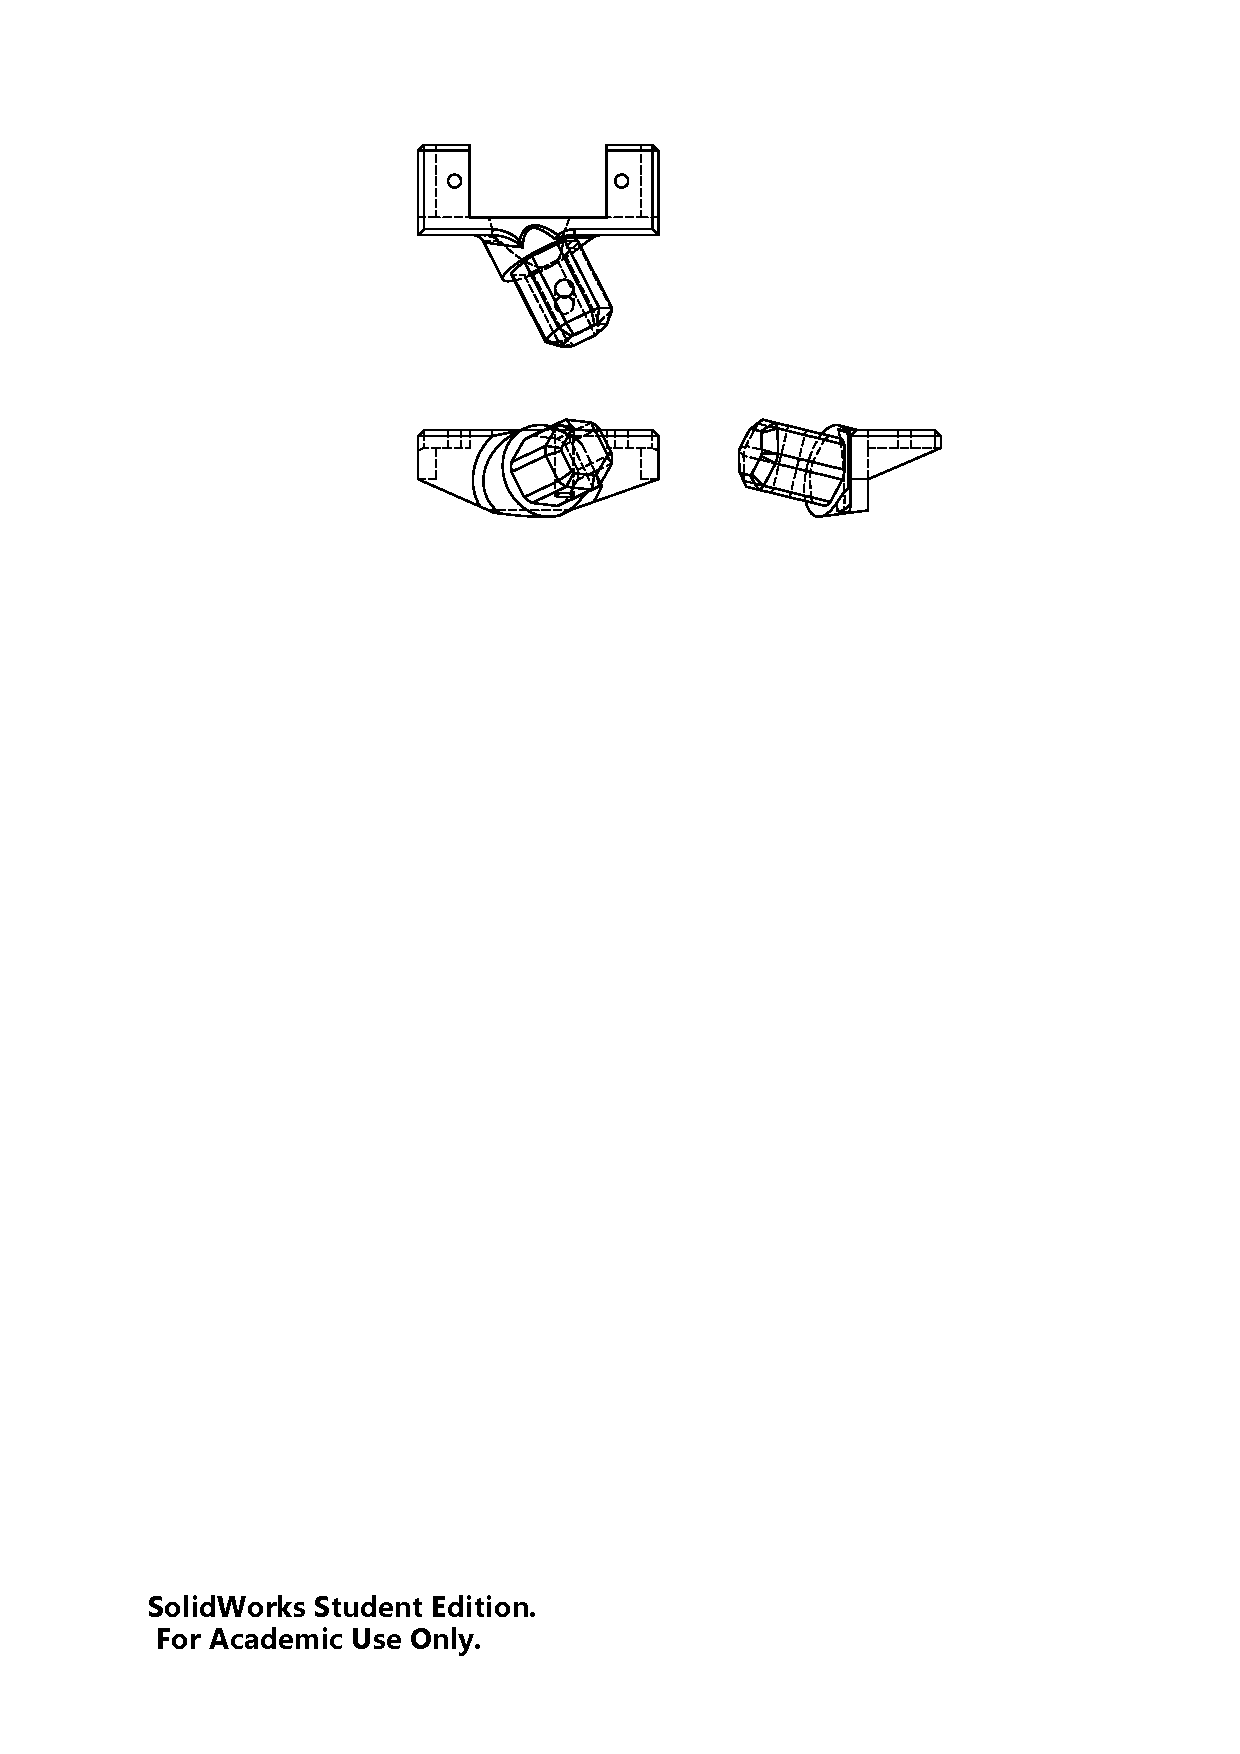
\includegraphics[clip, trim=6cm 20cm 4cm 2cm, width=0.55\linewidth]{figures/wheel-pivot}
        }
        \subfloat[]{
          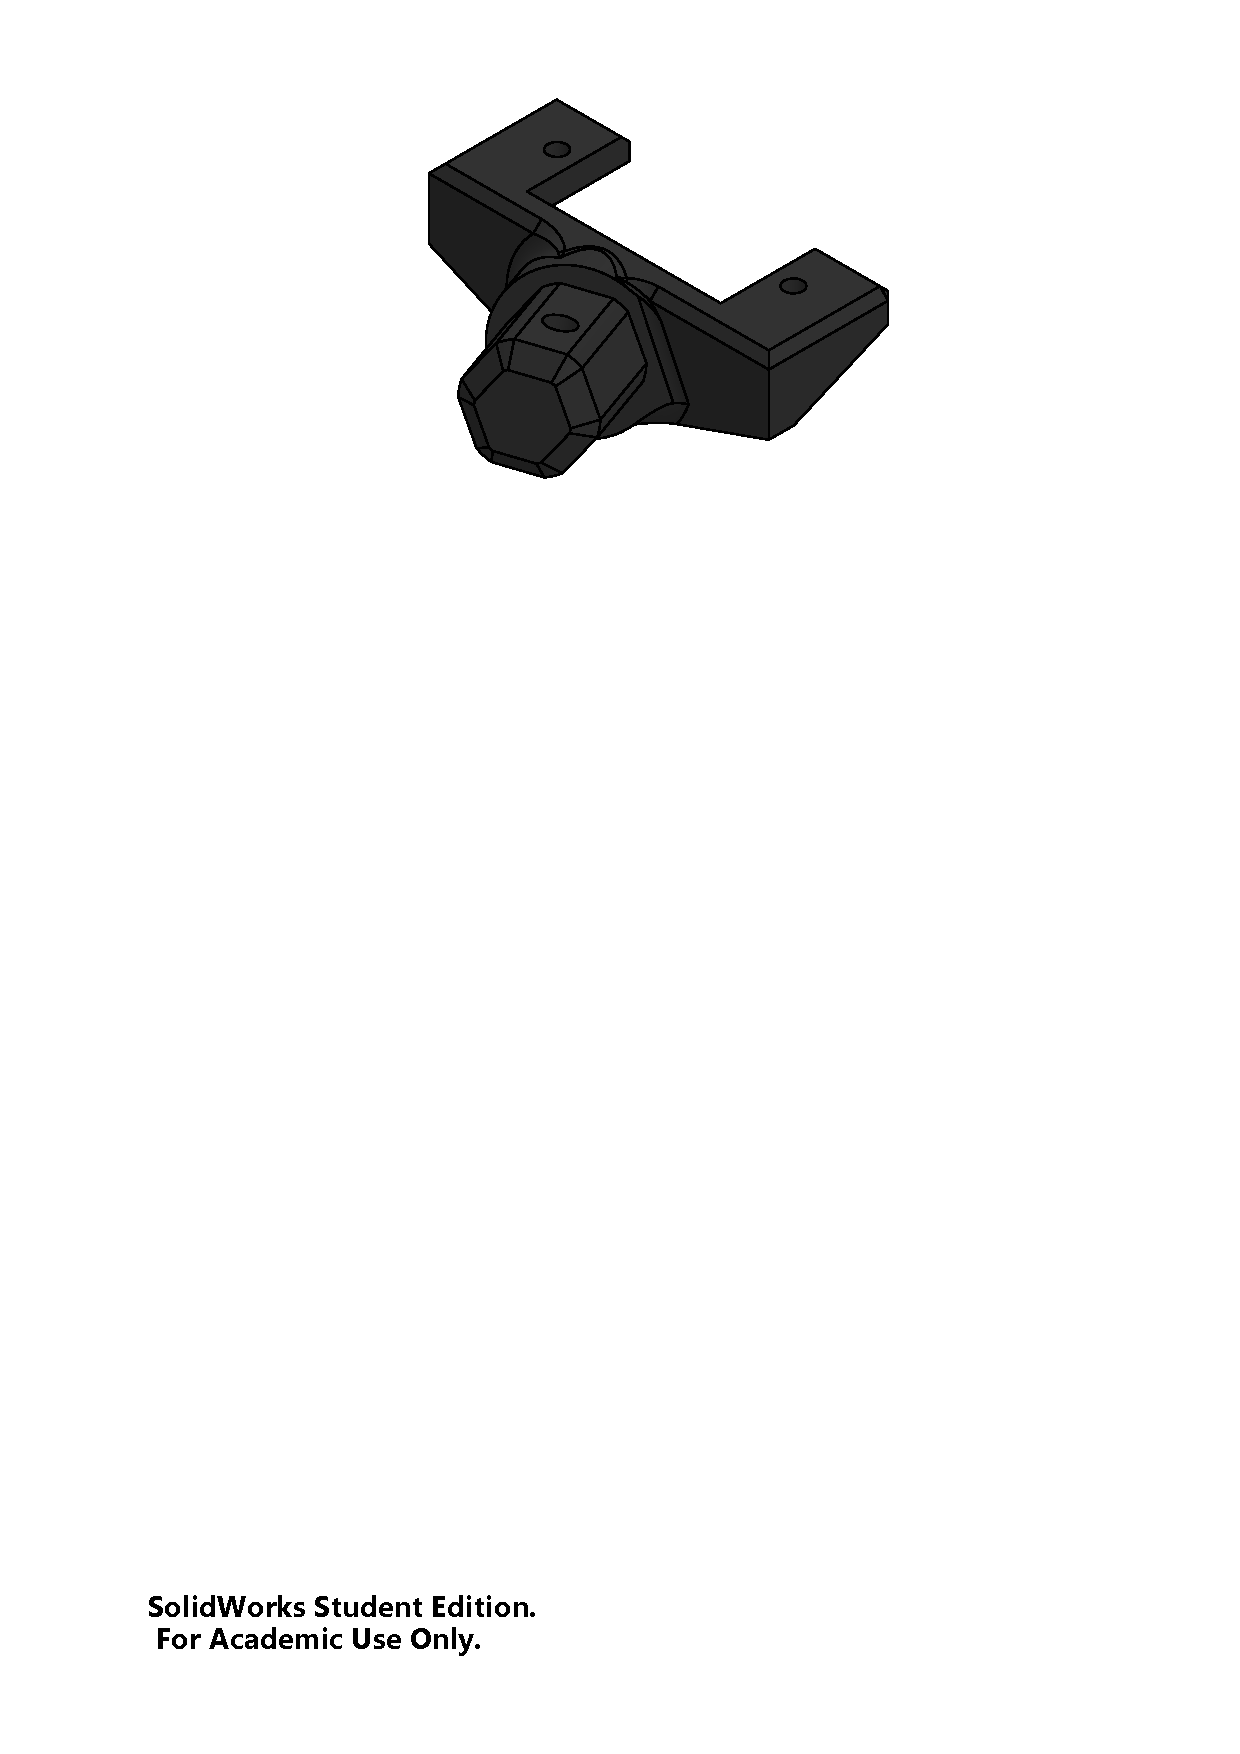
\includegraphics[clip, trim=6cm 20cm 5cm 1cm, width=0.44\linewidth]{figures/wheel-pivot-iso}
        }
        \caption[Detailed drawings of the wheel pivot component for one corner of the suspension system]{Detailed drawings of the wheel pivot component for one corner of the suspension system}
        \label{fig:mechDesign-wheelPivotDetail}
        \end{figure}
          
      \subheading{Struts}\\\\
        \textit{Curiosity} has an arcing ``strut'' for each wheel which curves from above the wheel, underneath the pivot motor, over the side and into the inwards-facing threshold of the hollow of the wheel. The strut is attached to the drive motor on the inside of the wheel, as close as possible to the centre of the wheel for balance and minimisation of bending stress. The sub-micro sized servos would not fit inside the wheels of the model at its chosen scale, thus they had to be mounted on the outside of the wheel. The strut was required to provide a place to mount the driving servo and to be mounted to the servo horns of the steering servo.
        
        The strut was designed to maintain the curved appearance as on \textit{Curiosity} but to take into account the strength of the component. A flat platform above the wheel included holes for mounting the steering servo's horn and this curved downwards into the strut section of the component. The strut curve consisted of a flat section to offer strength against bending in the typical direction as loaded (the $x$-axis) with a rib type extrusion from the rear-facing side of the strut for increased support and tabs on which to mount the driving servo. The design was then mirrored for the rest of the corners and the final detail can be seen in Figure~\ref{fig:mechDesign-wheelStrutDetail}.
        
        \begin{figure}[h!]
        \centering
        \subfloat[]{
          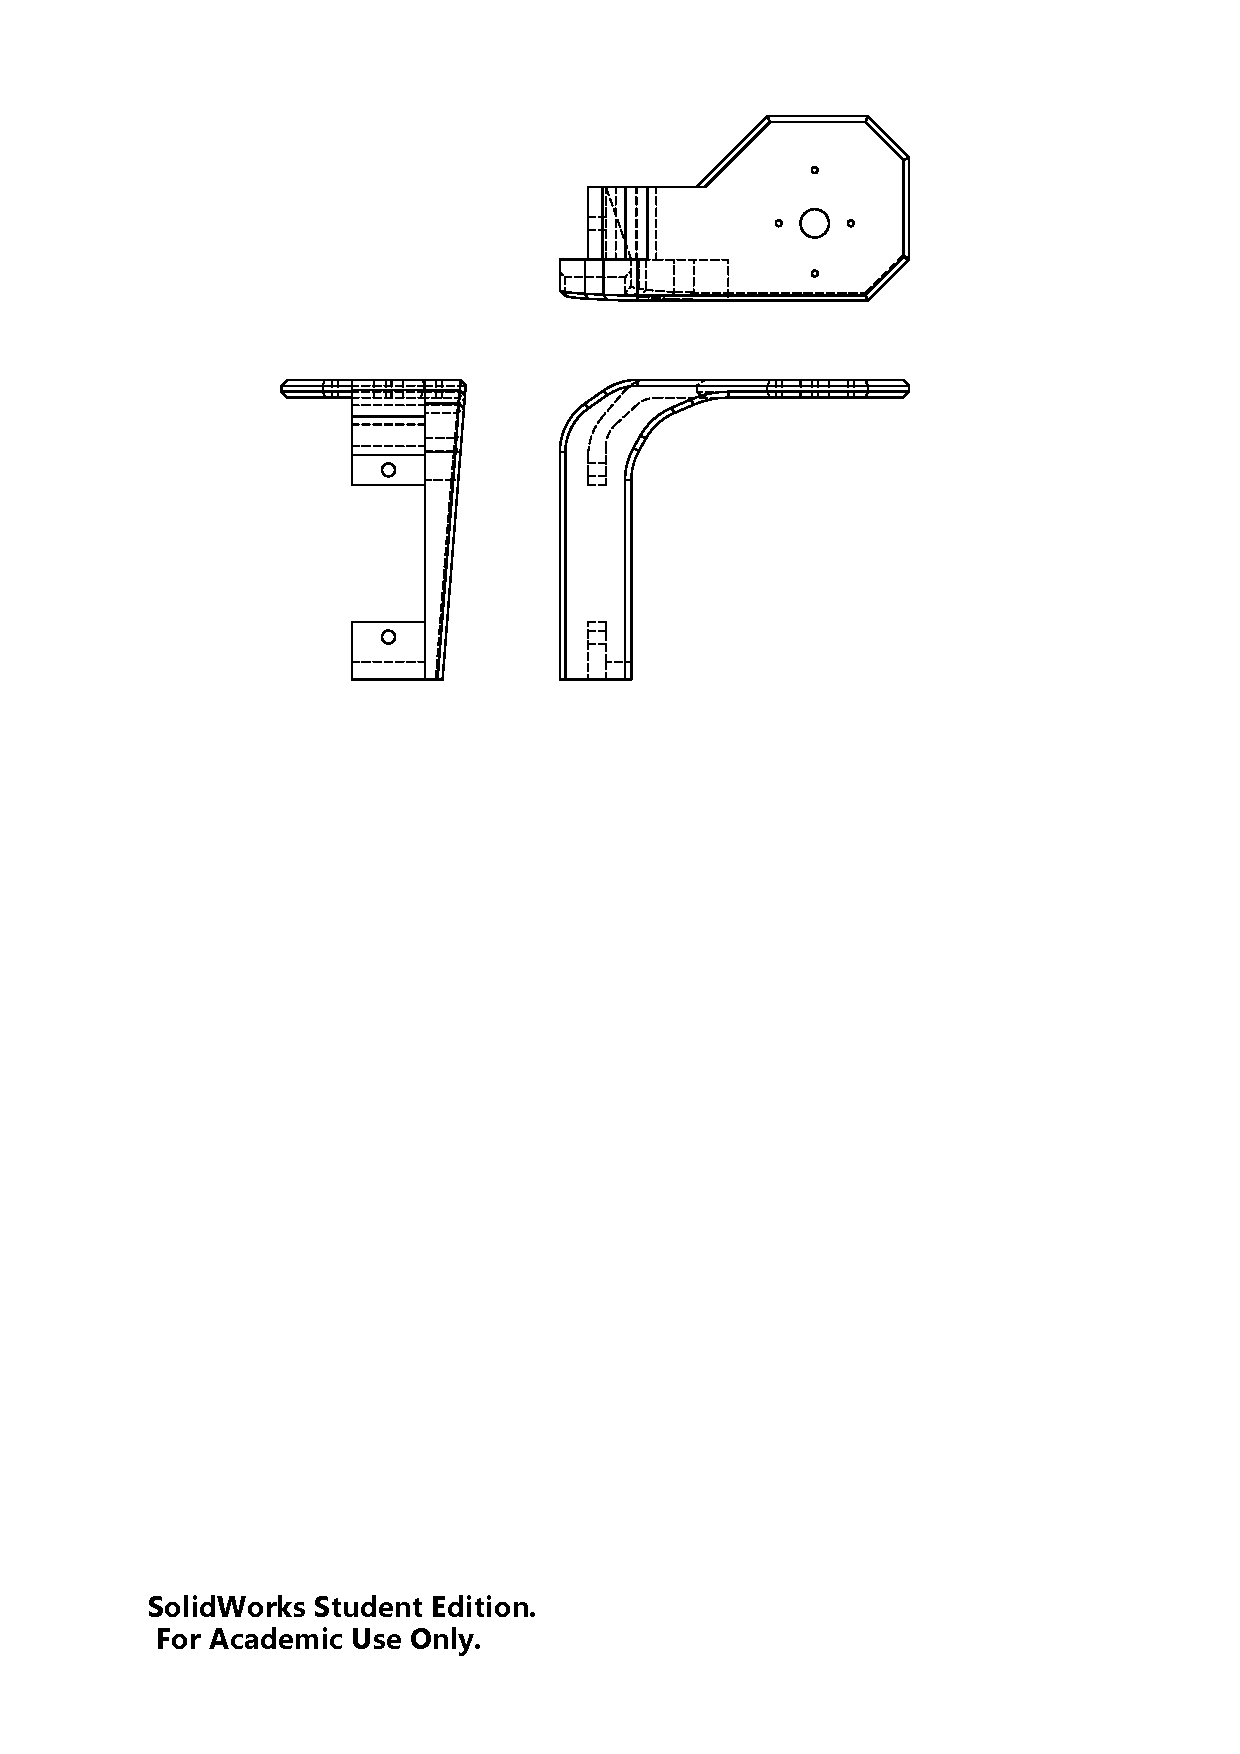
\includegraphics[clip, trim=4cm 17cm 4cm 2cm, width=0.59\linewidth]{figures/wheel-strut}
        }
        \subfloat[]{
          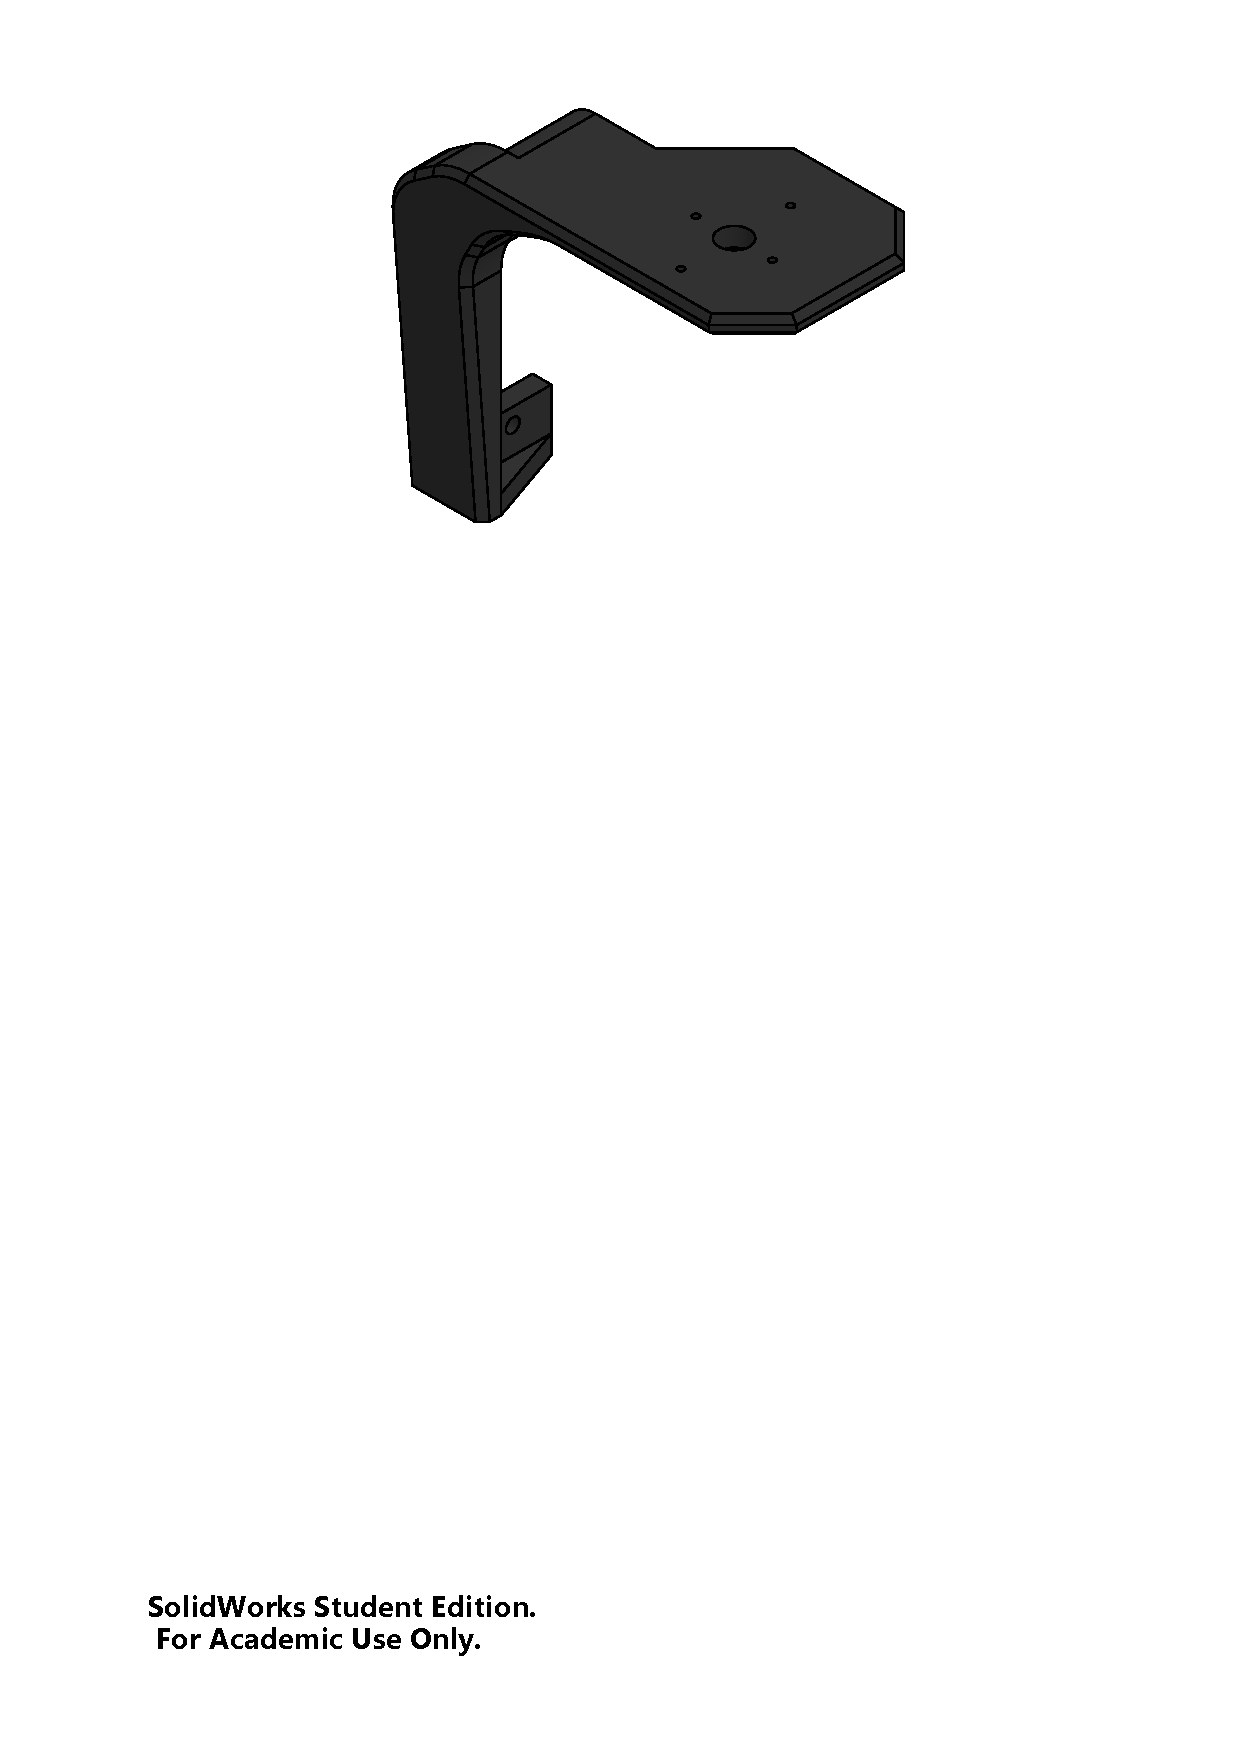
\includegraphics[clip, trim=6cm 19cm 5cm 1cm, width=0.4\linewidth]{figures/wheel-strut-iso}
        }
        \caption[Detailed drawings of the wheel pivot component for one corner of the suspension system]{Detailed drawings of the wheel pivot component for one corner of the suspension system}
        \label{fig:mechDesign-wheelStrutDetail}
        \end{figure}
          
      \subheading{Final Sub-assembly}  

      Having designed the parts around the skeleton sketch, where they were kept fixed to preserve the angle details linking them, another assembly was created, shown in Figure~\ref{fig:mechDesign-suspensionSubDetail} into which the parts were re-added and mated in a manner more typical of the way that they would be assembled. The assembly allowed simulation of the movement and this functionality was used to analyse the assembly for interferences and to ensure that the structure moved the way it was required. Figure~\ref{fig:mechDesign-suspensionSubObstacle} shows the linkages positioned as if the subsystem was navigating over an obstacle. Each individual part was then mirrored and assembled to form the opposite side of the suspension system. The CAD package ensured that the mirrored parts were dynamically updated should one of the original parts have changed.
      
      \begin{figure}[h!]
      \centering
      \subfloat[]{
        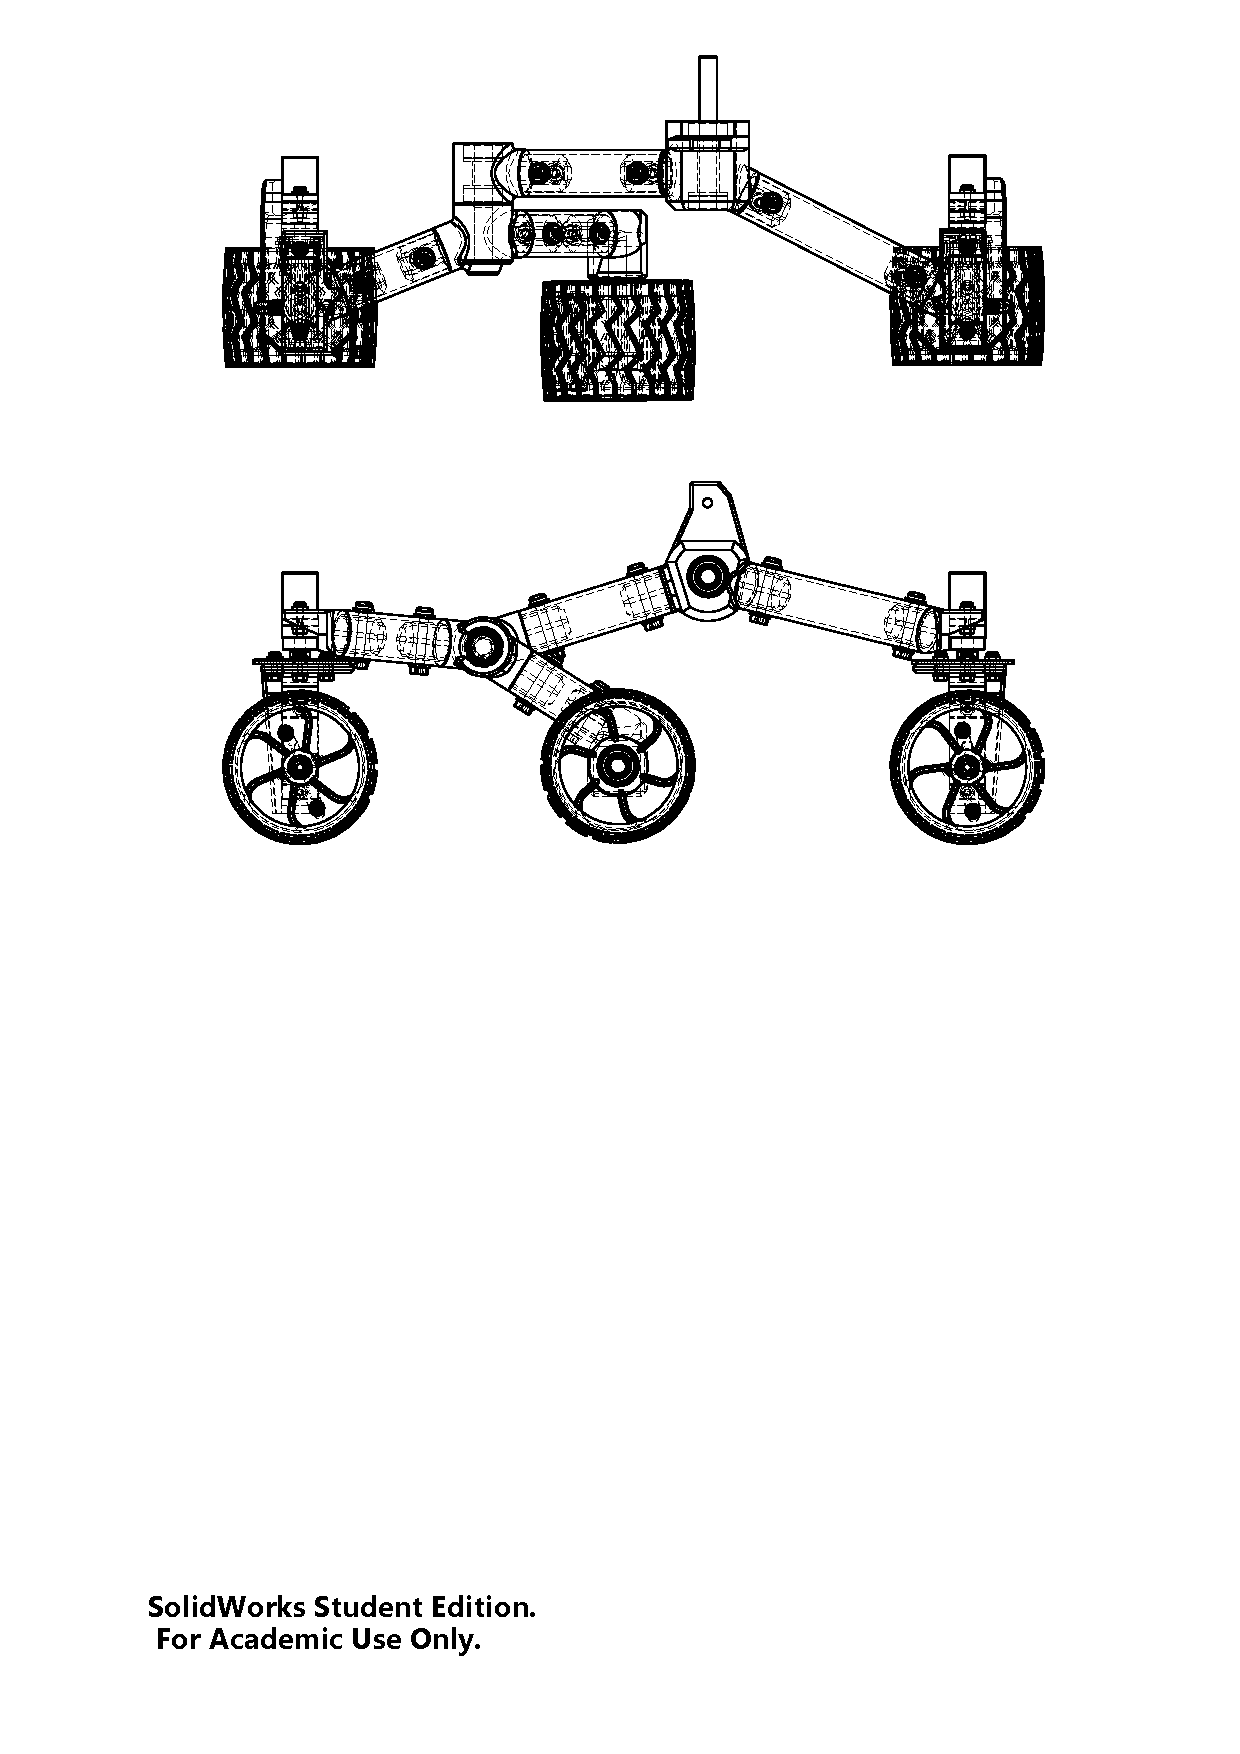
\includegraphics[clip, trim=2cm 15cm 2cm 1cm, width=0.9\linewidth]{figures/suspensionSub}
      }
      \qquad
      \subfloat[]{
        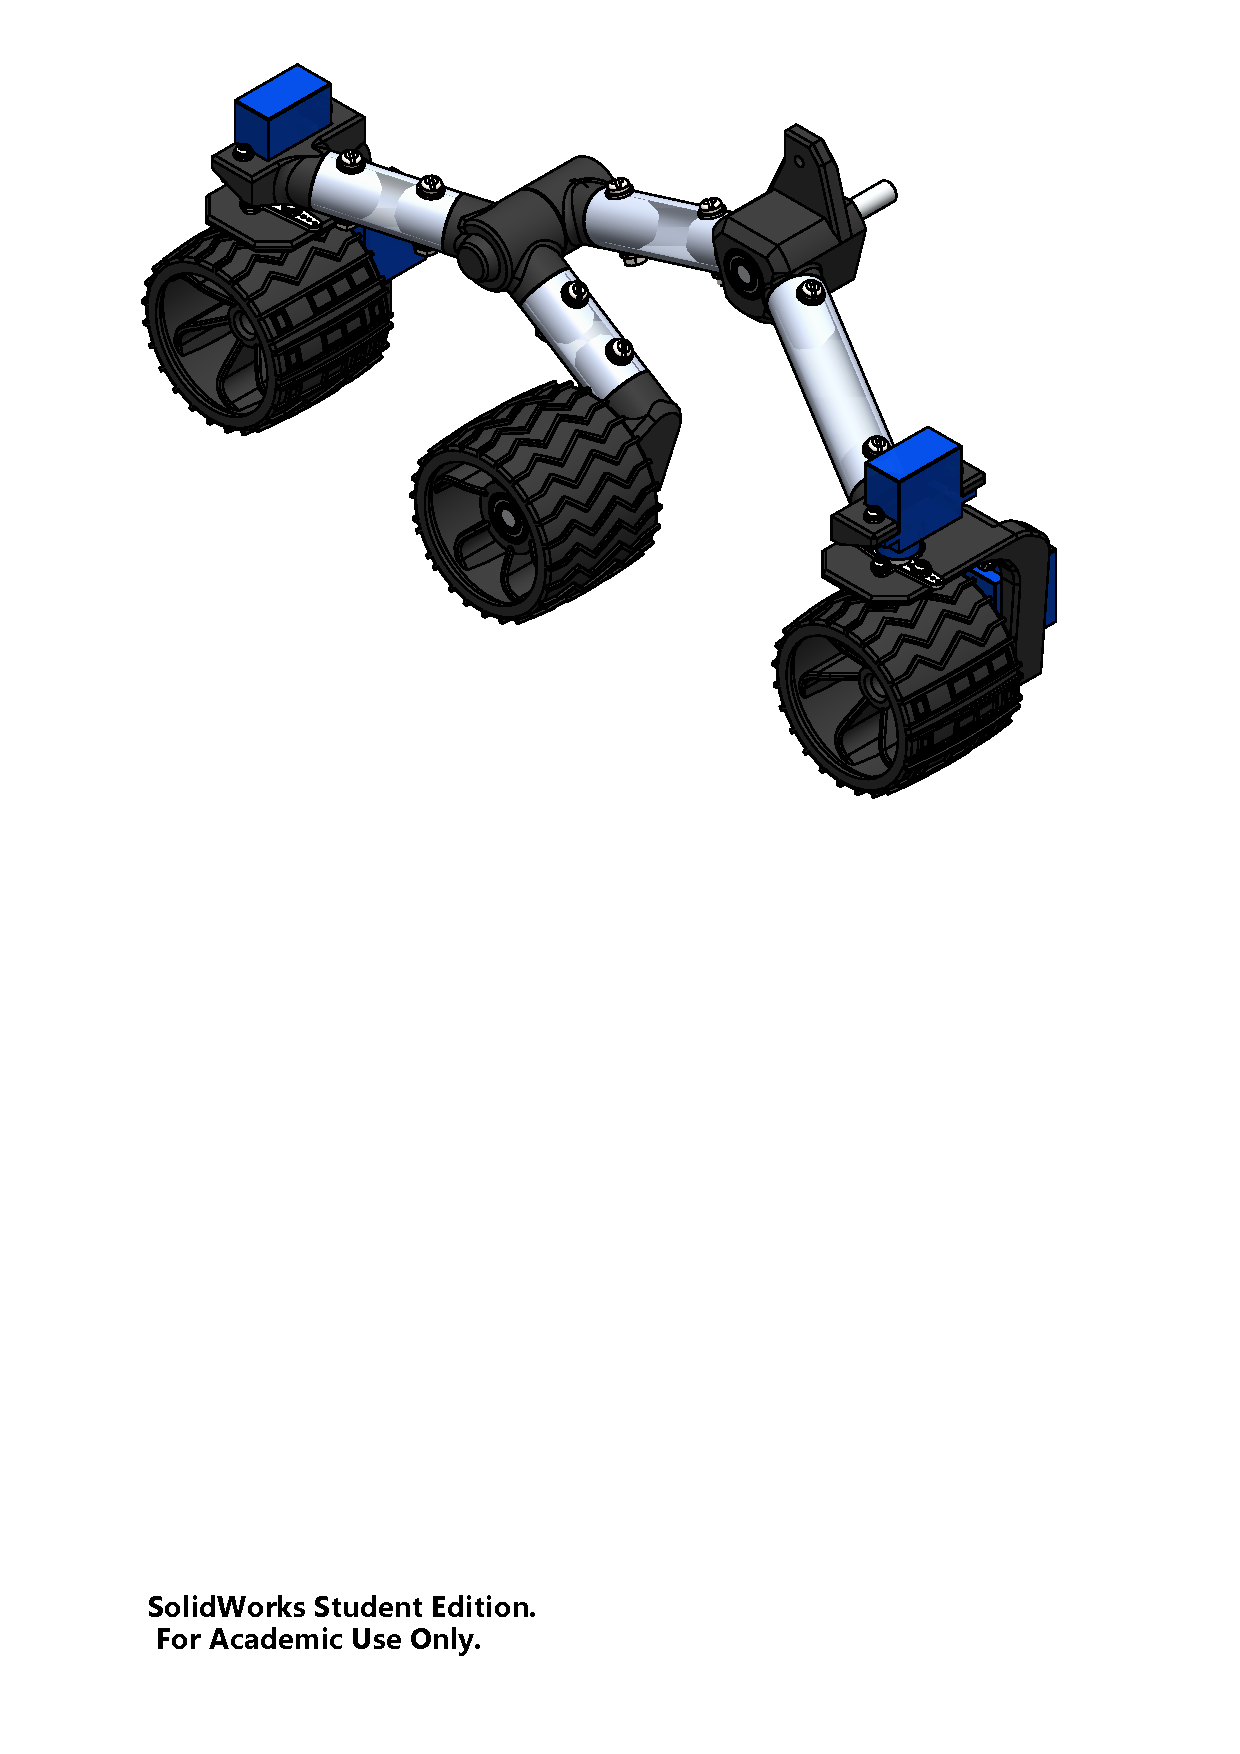
\includegraphics[clip, trim=2cm 15cm 2cm 1cm, width=0.7\linewidth]{figures/suspensionSub-iso}
      }
      \caption[Detailed drawings of the working, dynamic assembly one side of the suspension system]{Detailed drawings of the working, dynamic assembly one side of the suspension system}
      \label{fig:mechDesign-suspensionSubDetail}
      \end{figure}
      
      \begin{figure}[h!]
        \centering
        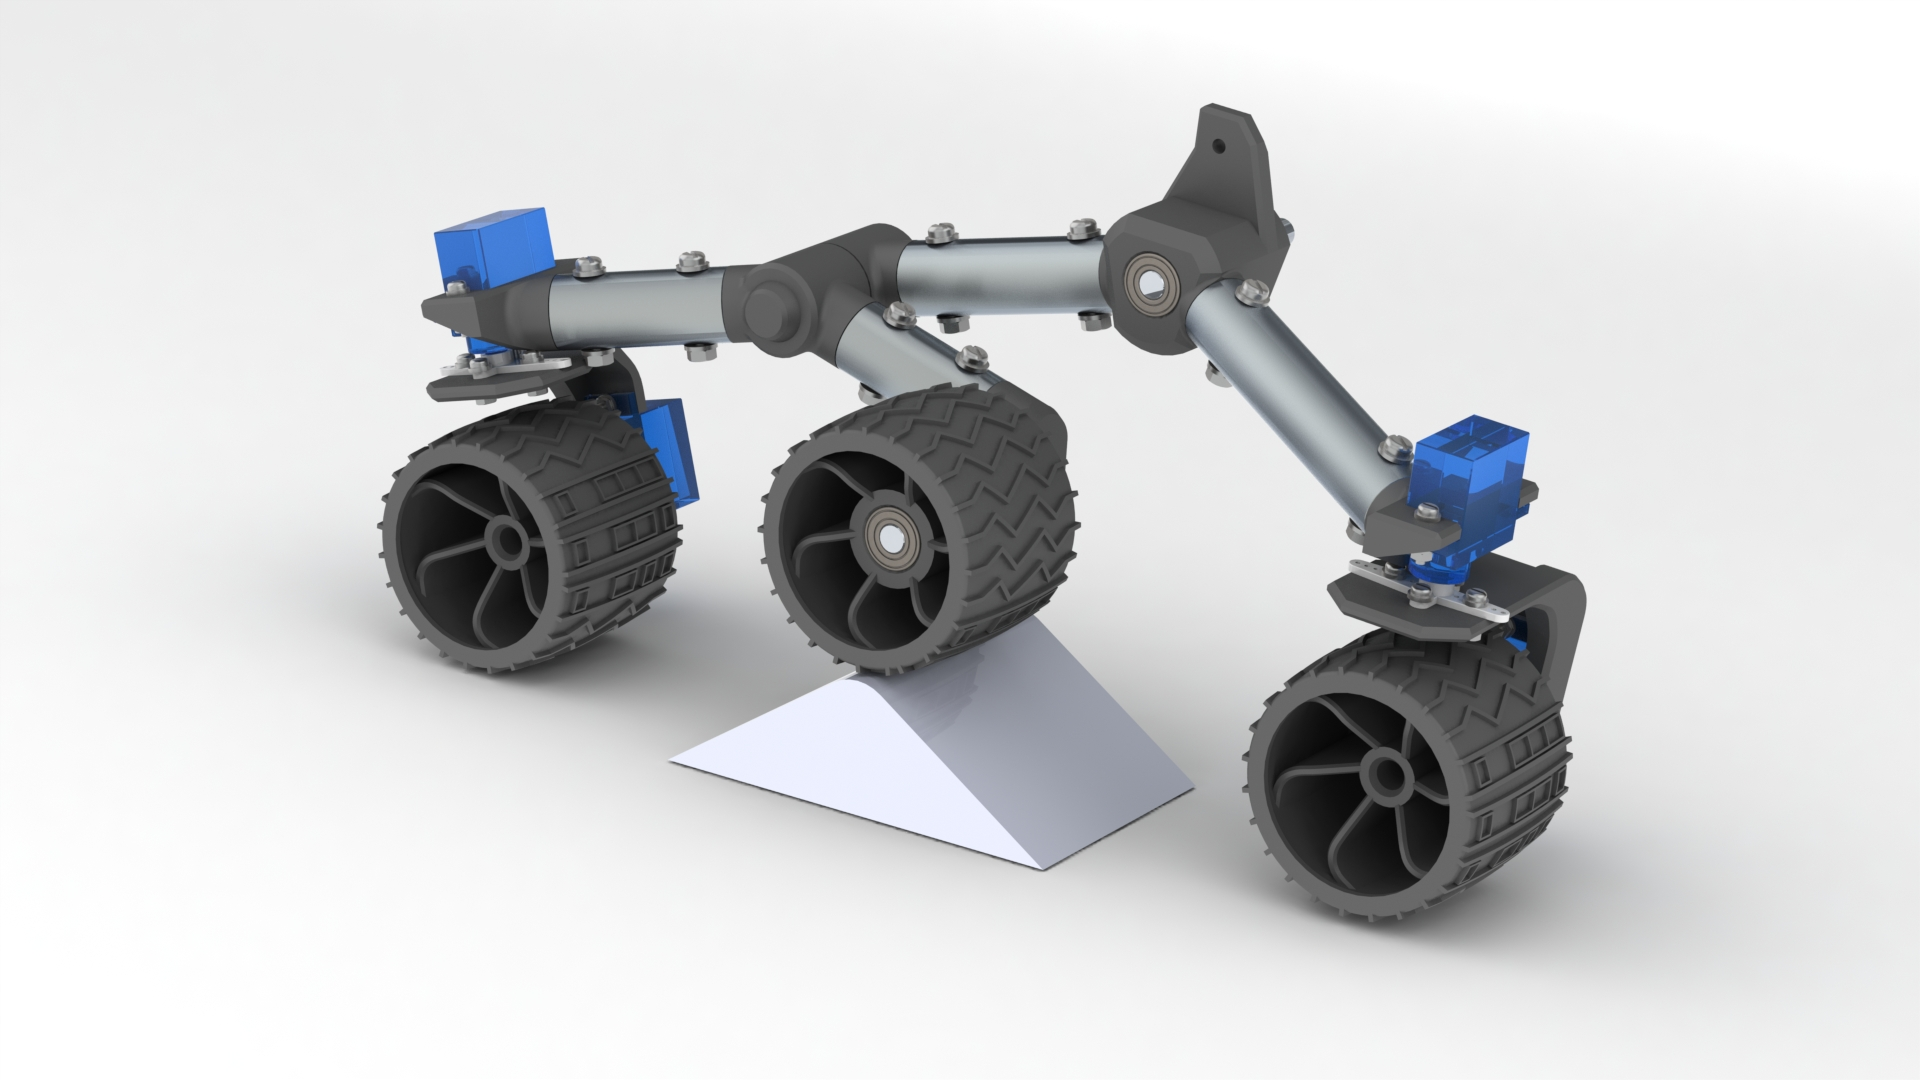
\includegraphics[width=1\linewidth]{figures/suspensionSub-obstacle}
        \caption[Render of one side of the suspension system navigating over an obstacle]{Render of one side of the suspension system navigating over an obstacle}
        \label{fig:mechDesign-suspensionSubObstacle}
      \end{figure}
      
    \subsubsection{Differential}
      Design of the differential involved a partially completed design of the body structure which contained details of the mounting points of the suspension system and thus the position of the connection point on the rocker joint, as well as the centre point of articulation of the differential bar as acquired from the reference model. The concept chosen for this subsystem included a 3D printed differential bar, printed hinges and threaded-bar (rods) attached to the hinges to link the differential to the rocker joint. The need for hinges was to provide the rods with the degrees of freedom required taking into the account the arced motions of an end of the differential bar in the $x$-$y$-plane and rocker joint in the $x$-$z$-plane. The articulation of the differential system and the resulting motion of the rods is depicted in Figure~\ref{fig:mechDesign-differentialMotion}, each of the two views showing two positions in the motion.
      
      \begin{figure}[h!]
      \centering
      \subfloat[Top view\label{fig:mechDesign-differentialMotion-a}]{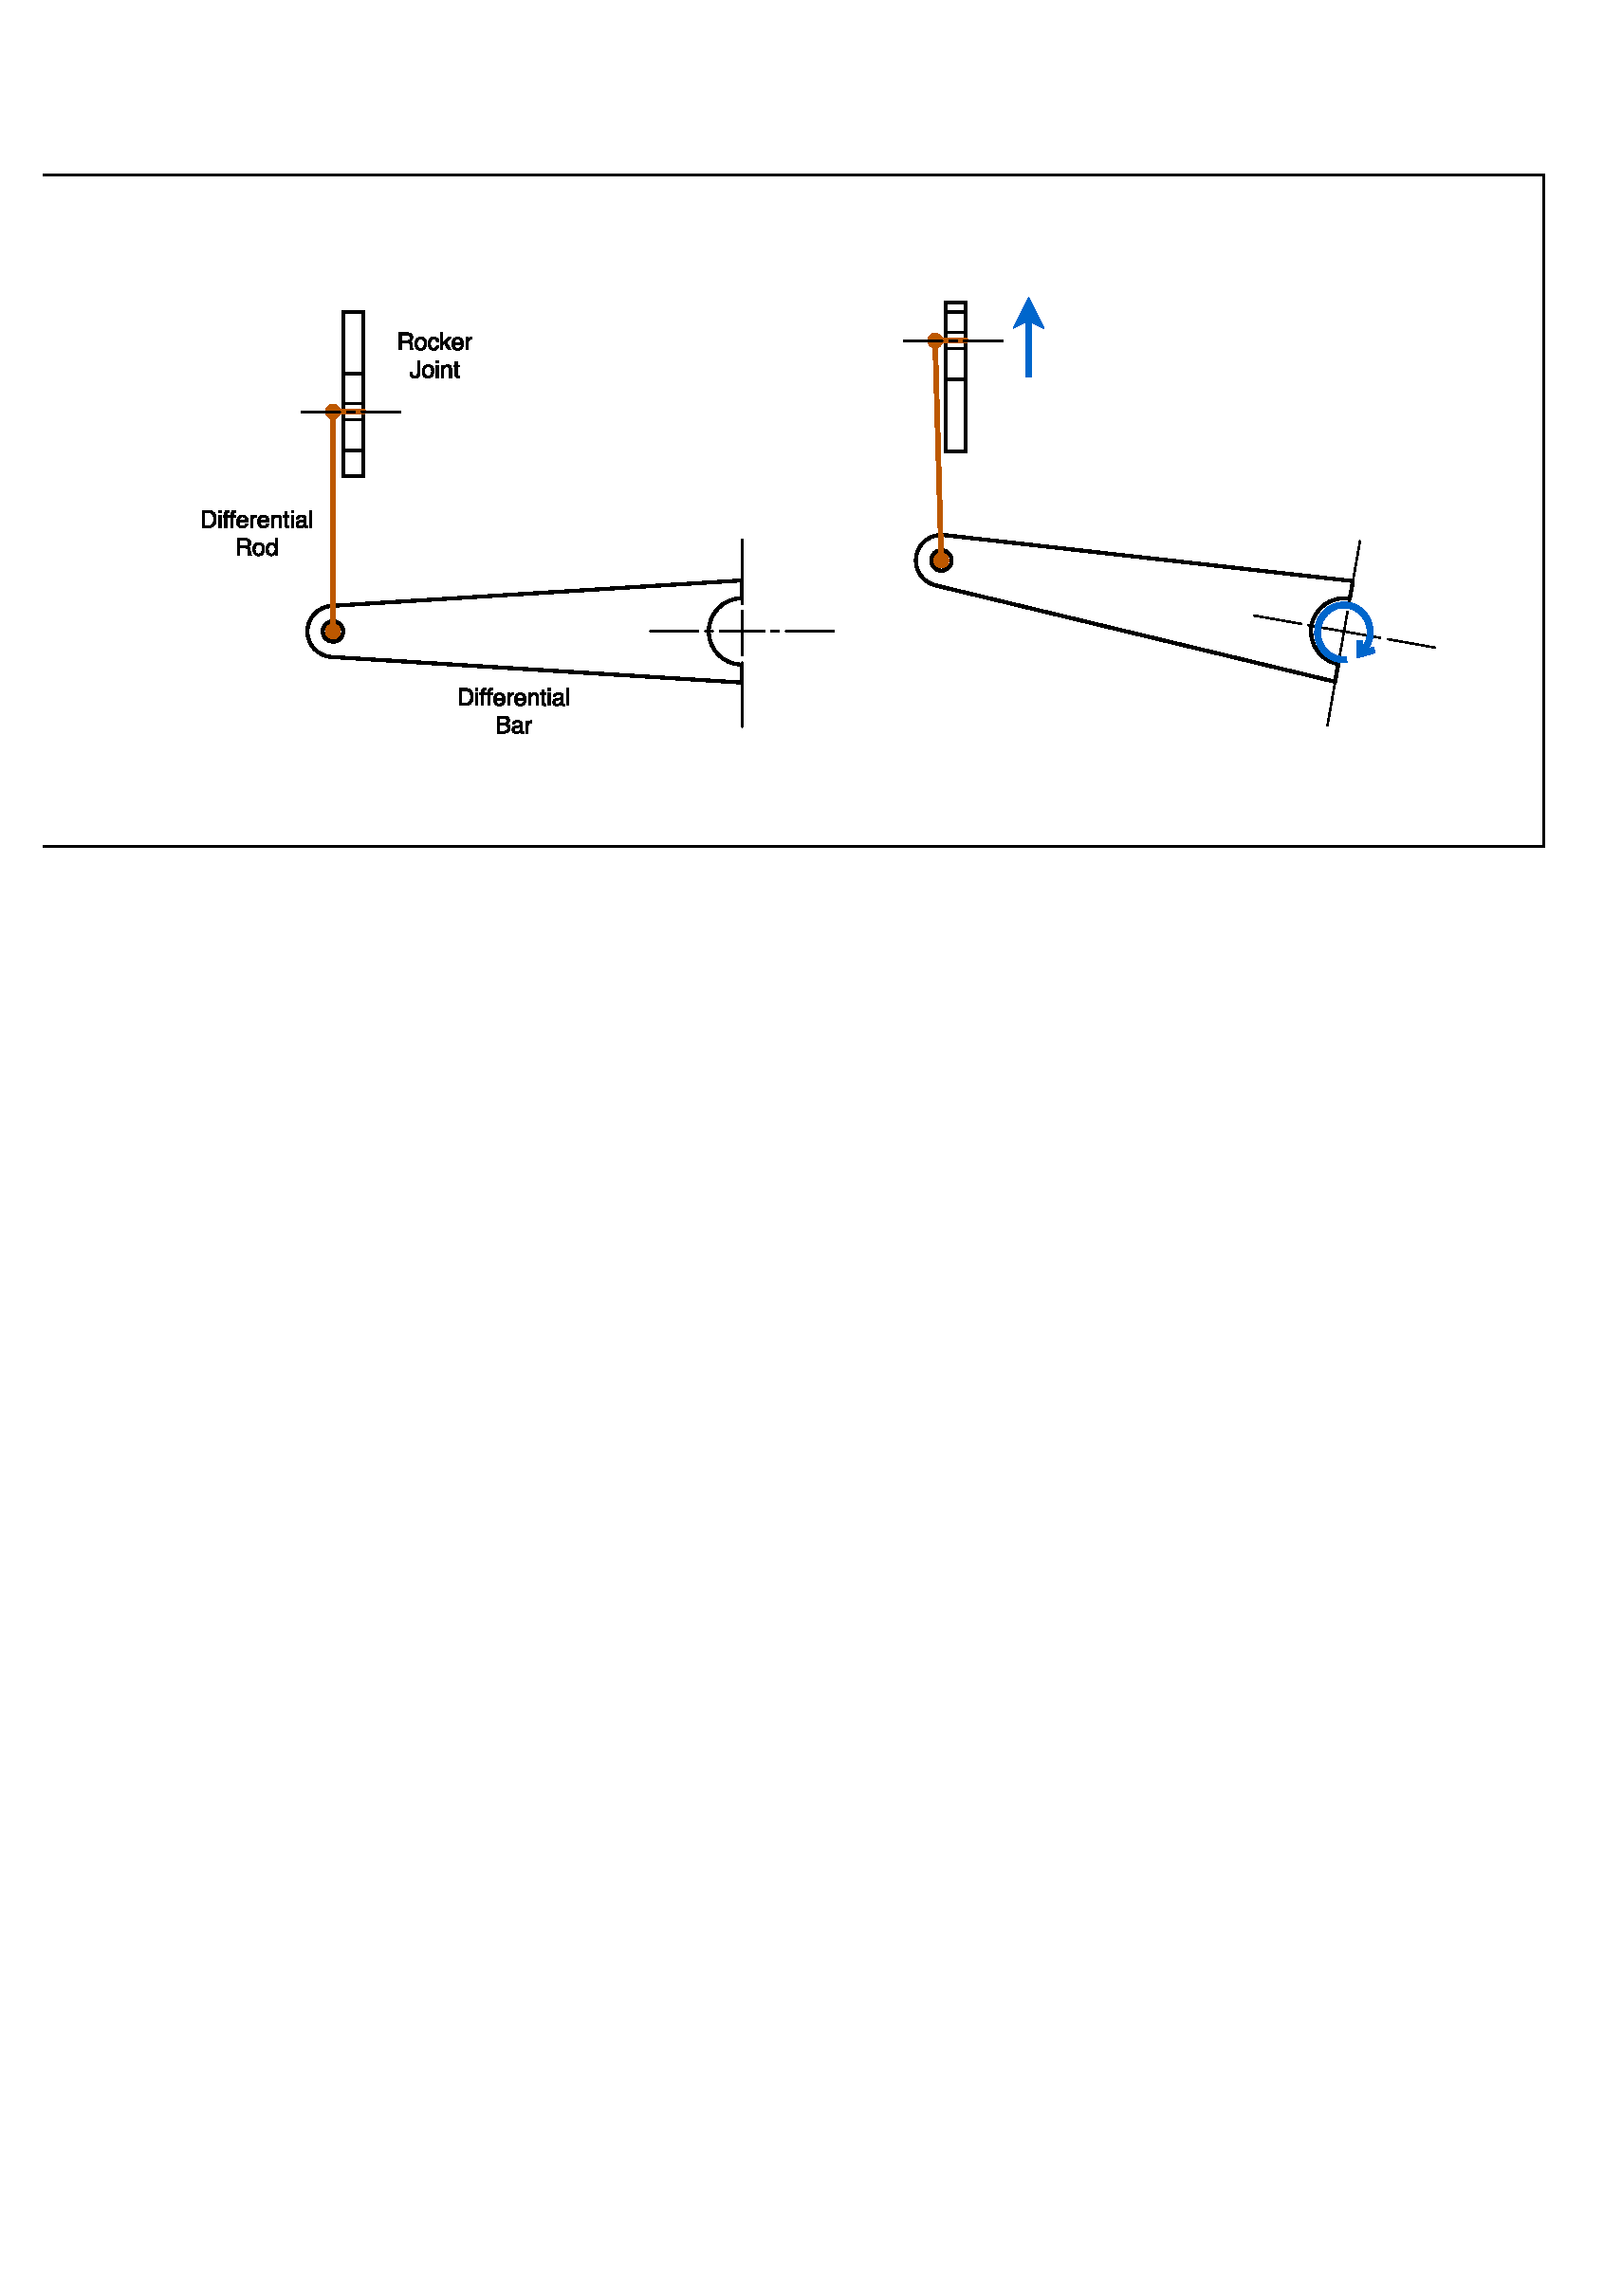
\includegraphics[clip, trim=2cm 26cm 2cm 4cm, width=0.9\linewidth]{figures/mechDesign-differentialMotionTop.pdf}}
      \qquad
      \subfloat[Side view]{
        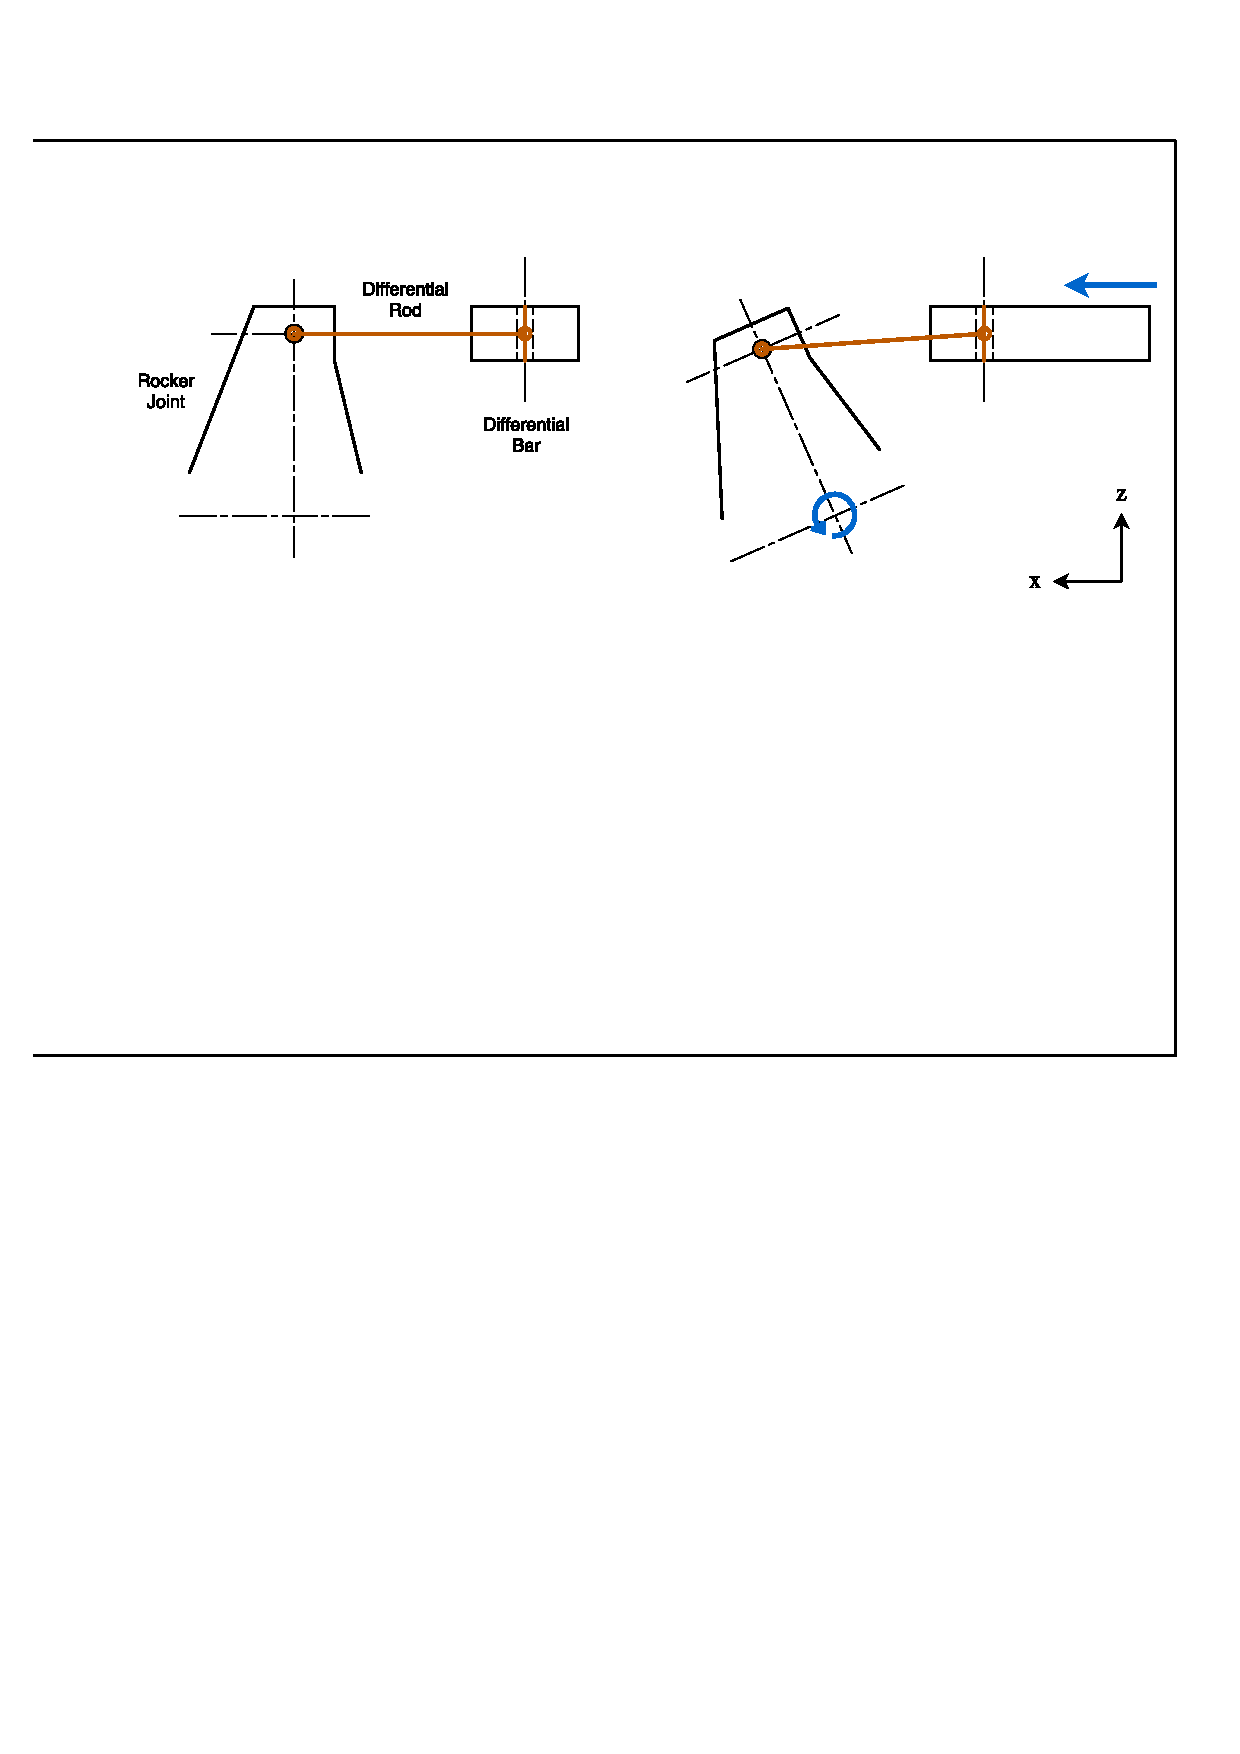
\includegraphics[clip, trim=2cm 26cm 2cm 4cm, width=0.9\linewidth]{figures/mechDesign-differentialMotionSide.pdf}
      }
      \caption[Diagram showing the motion of the differential and the resulting motion of the differential rod]{Diagram showing the motion of the differential and the resulting motion of the differential rod}
      \label{fig:mechDesign-differentialMotion}
      \end{figure}
      
      % TODO: Add axes to the above figure
      
      \subheading{Differential Bar}\\\\
        The design of the differential bar stemmed from the partially completed rover deck, specifically with respect to the width of the body and therefore the span of the rocker joints' differential connection points. The bar took on the tapered shape as on \textit{Curiosity} with the wider section in the centre and narrower ends. A hole was added for the addition of a bearing in the centre of the bar and holes for the hinges added to the ends. The bearing was to be mounted to a short shaft which was to be fixed into the deck of the rover. Figure~\ref{fig:mechDesign-differentialBarDetail} shows the detail of the differential bar.
        
        \begin{figure}[h!]
        \centering
        \subfloat[]{
          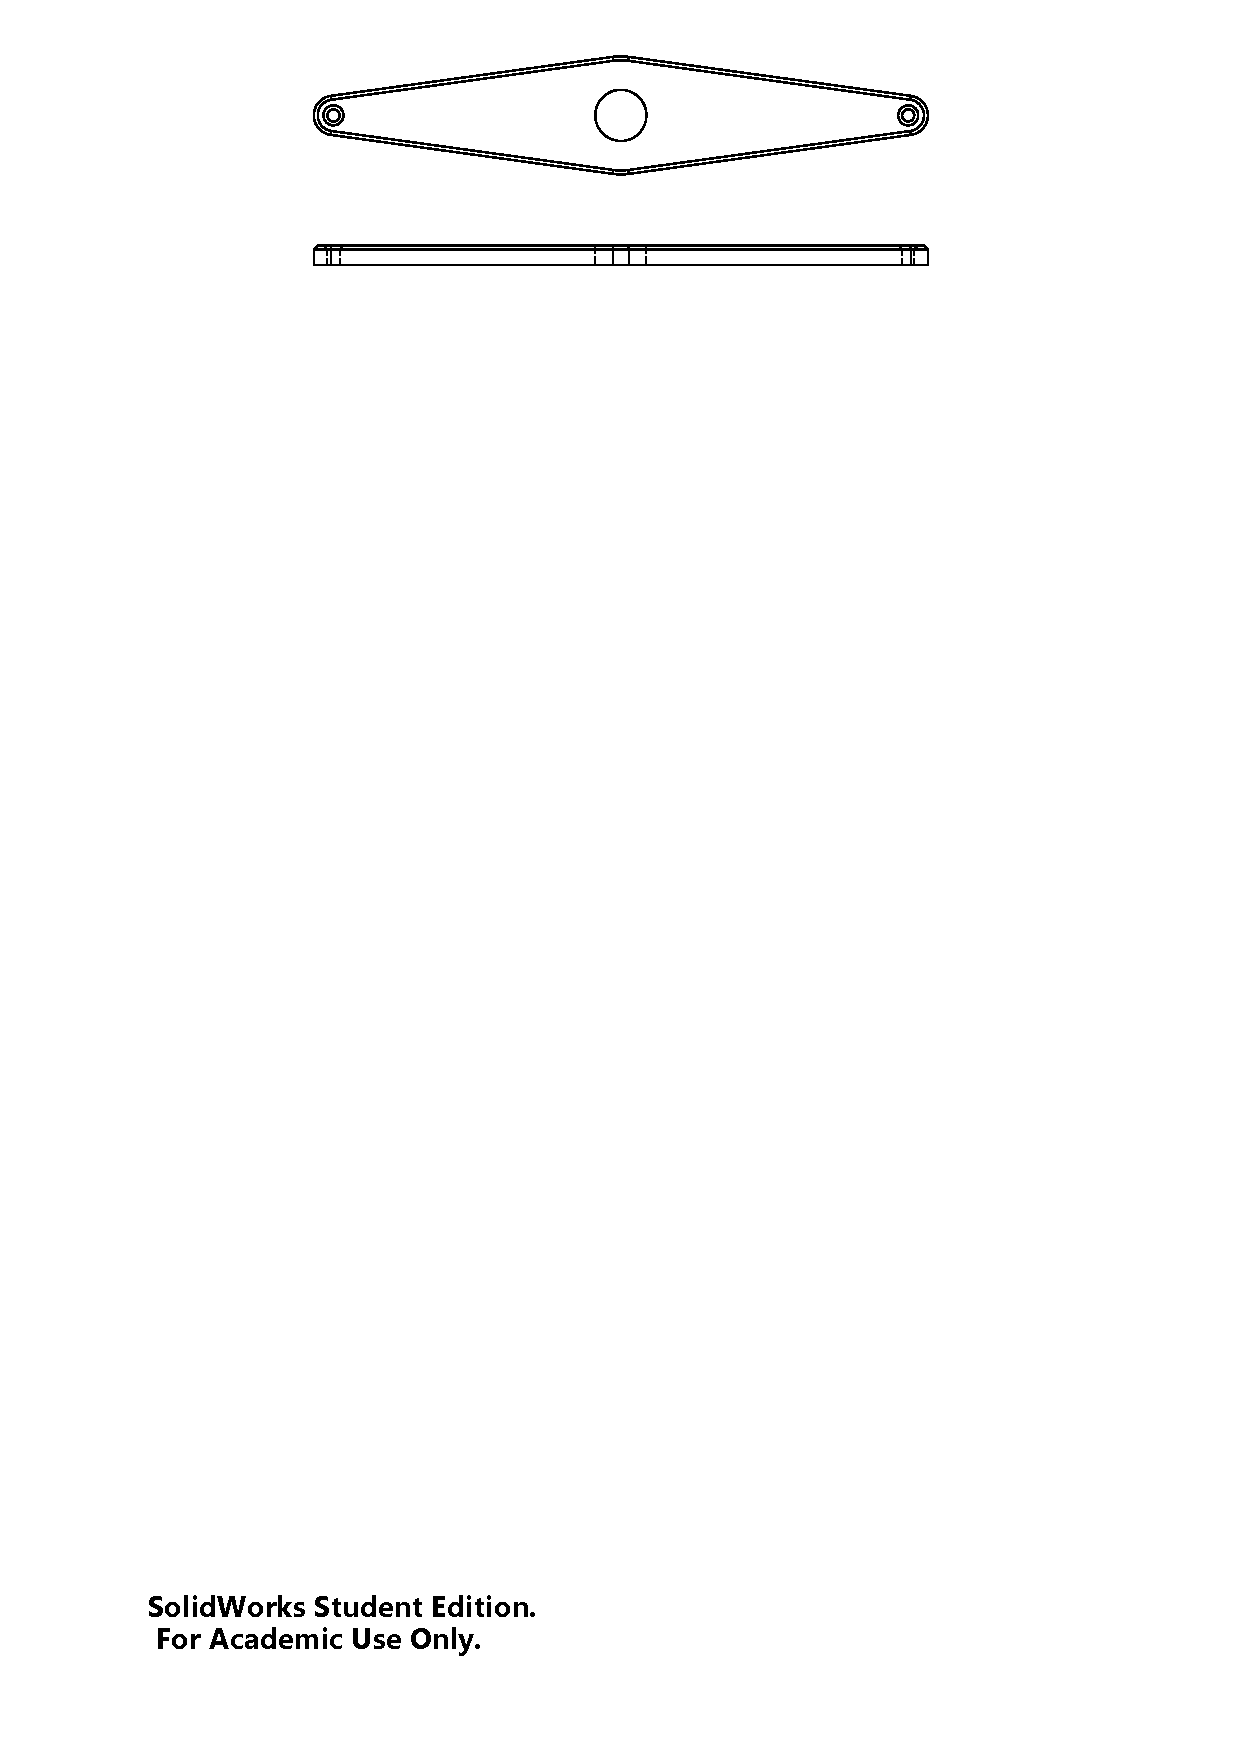
\includegraphics[clip, trim=5cm 24cm 5cm 0cm, width=0.5\linewidth]{figures/differential-bar}
        }%
        \subfloat[]{
          
\includegraphics[clip, trim=3cm 21cm 3cm 1cm, width=0.49\linewidth]{figures/differential-bar-iso}
        }
        \caption[Detailed drawings of the differential bar component in the differential system]{Detailed drawings of the differential bar component in the differential system}
        \label{fig:mechDesign-differentialBarDetail}
        \end{figure}
        
        
      \subheading{Hinges}\\\\
        Hinges were designed for each end of the rods, one end on the rocker joint side and the other for the differential bar. The hinges allowed rotation about specific axes, the $y$- and $z$-axes on the bar side and the $y$-axis on the joint side. Figure~\subref*{fig:mechDesign-differentialMotion-a} demonstrates that the bar also rotates about the $z$-axis which would require the hinge at the rocker joint to allow for this motion. However, this was not included in the design after confirming through calculation that the amount by which the bar would have rotated in this direction at the maximum angle of articulation of the differential bar ($\approx9^\circ$) did not justify the resulting added complexity in the hinge design.
        
        The single axis hinge on the rocker joint side amounted to a right-angled piece with a hole in one of the flat sections for fastening it to the rocker joint and another hole on the other flat section for fastening of the threaded-bar rod component. Slotted bolts and nuts were used for the joint hole, with washers between the joint and the hinge part to minimise the friction between the parts despite a small degree of motion that would be effected on this coupling. For the rod, two nuts on either side of the piece were used to fix the threaded-bar.
        
        The two-axis hinge on the differential-bar end included a part with two tabs with holes, one above and one below the end of the bar and a flat section extending perpendicular to the axis made between the two tab-holes. The additional section included a third hole to allow attachment of the second part used for mounting the rod. The second component included a blind hole into which the rod could be place and a cutout halfway down the length of the hole to allow for a nut to be pushed into place. This meant that the rod could be screwed into the piece, the purpose of which included easy assembly and breakdown if required as well as allowing the extension of the rod to be adjusted. Therefore, the differential system could be adjusted to balance the rover body about the rocker joint pivot points.
        
        Detailed drawings of both hinge assemblies can be seen in Figures~\ref{fig:mechDesign-singleAxisHingeDetail} and \ref{fig:mechDesign-twoAxisHingeDetail}.
        
        \begin{figure}[h!]
        \centering
        \subfloat[]{
          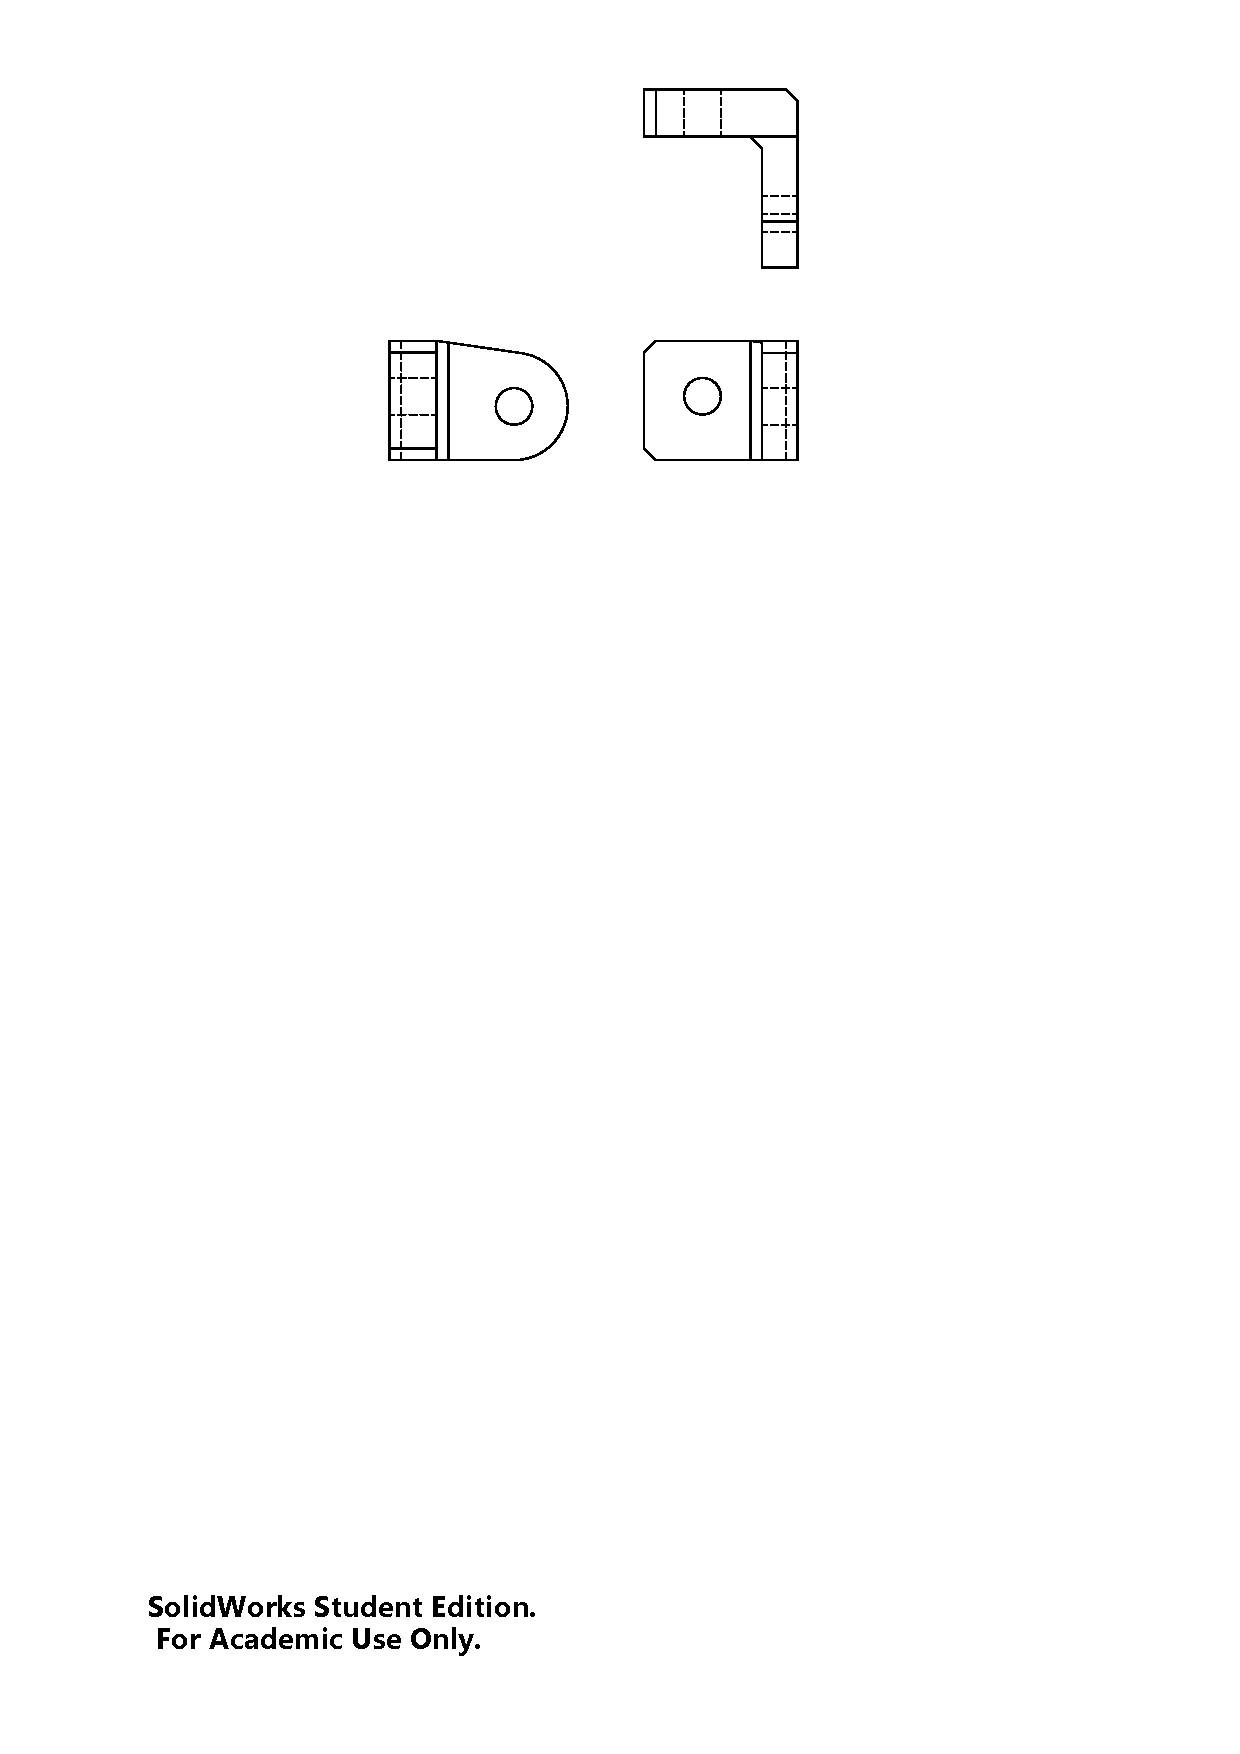
\includegraphics[clip, trim=9cm 24cm 6cm 0cm, width=0.4\linewidth]{figures/rod-hing-jointSide}
        }
        \qquad
        \subfloat[]{
          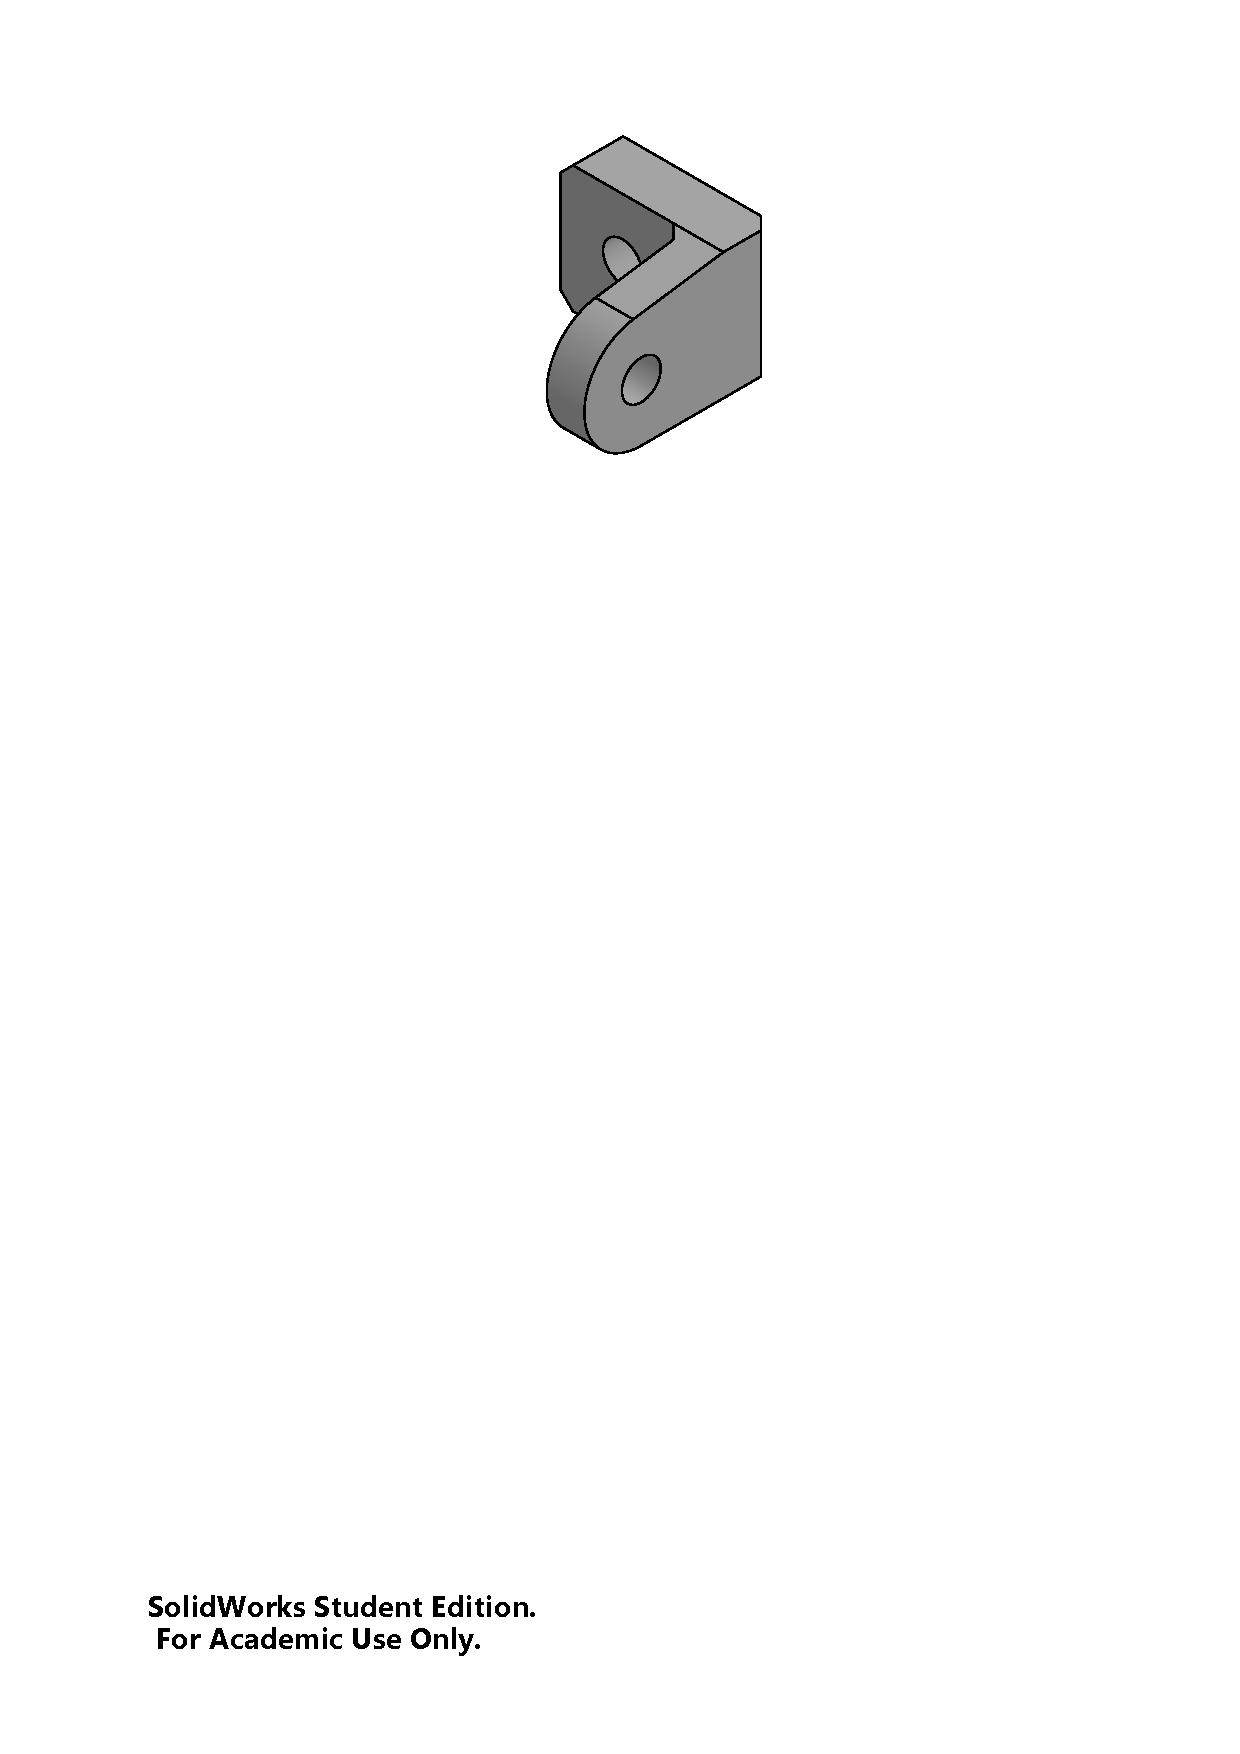
\includegraphics[clip, trim=5cm 20cm 5cm 1cm, width=0.4\linewidth]{figures/rod-hing-jointSide-iso}
        }
        \caption[Detailed drawings of the single-axis hinge component in the differential system]{Detailed drawings of the single-axis hinge component in the differential system}
        \label{fig:mechDesign-singleAxisHingeDetail}
        \end{figure}
        
        \begin{figure}[h!]
        \centering
        \subfloat[]{
          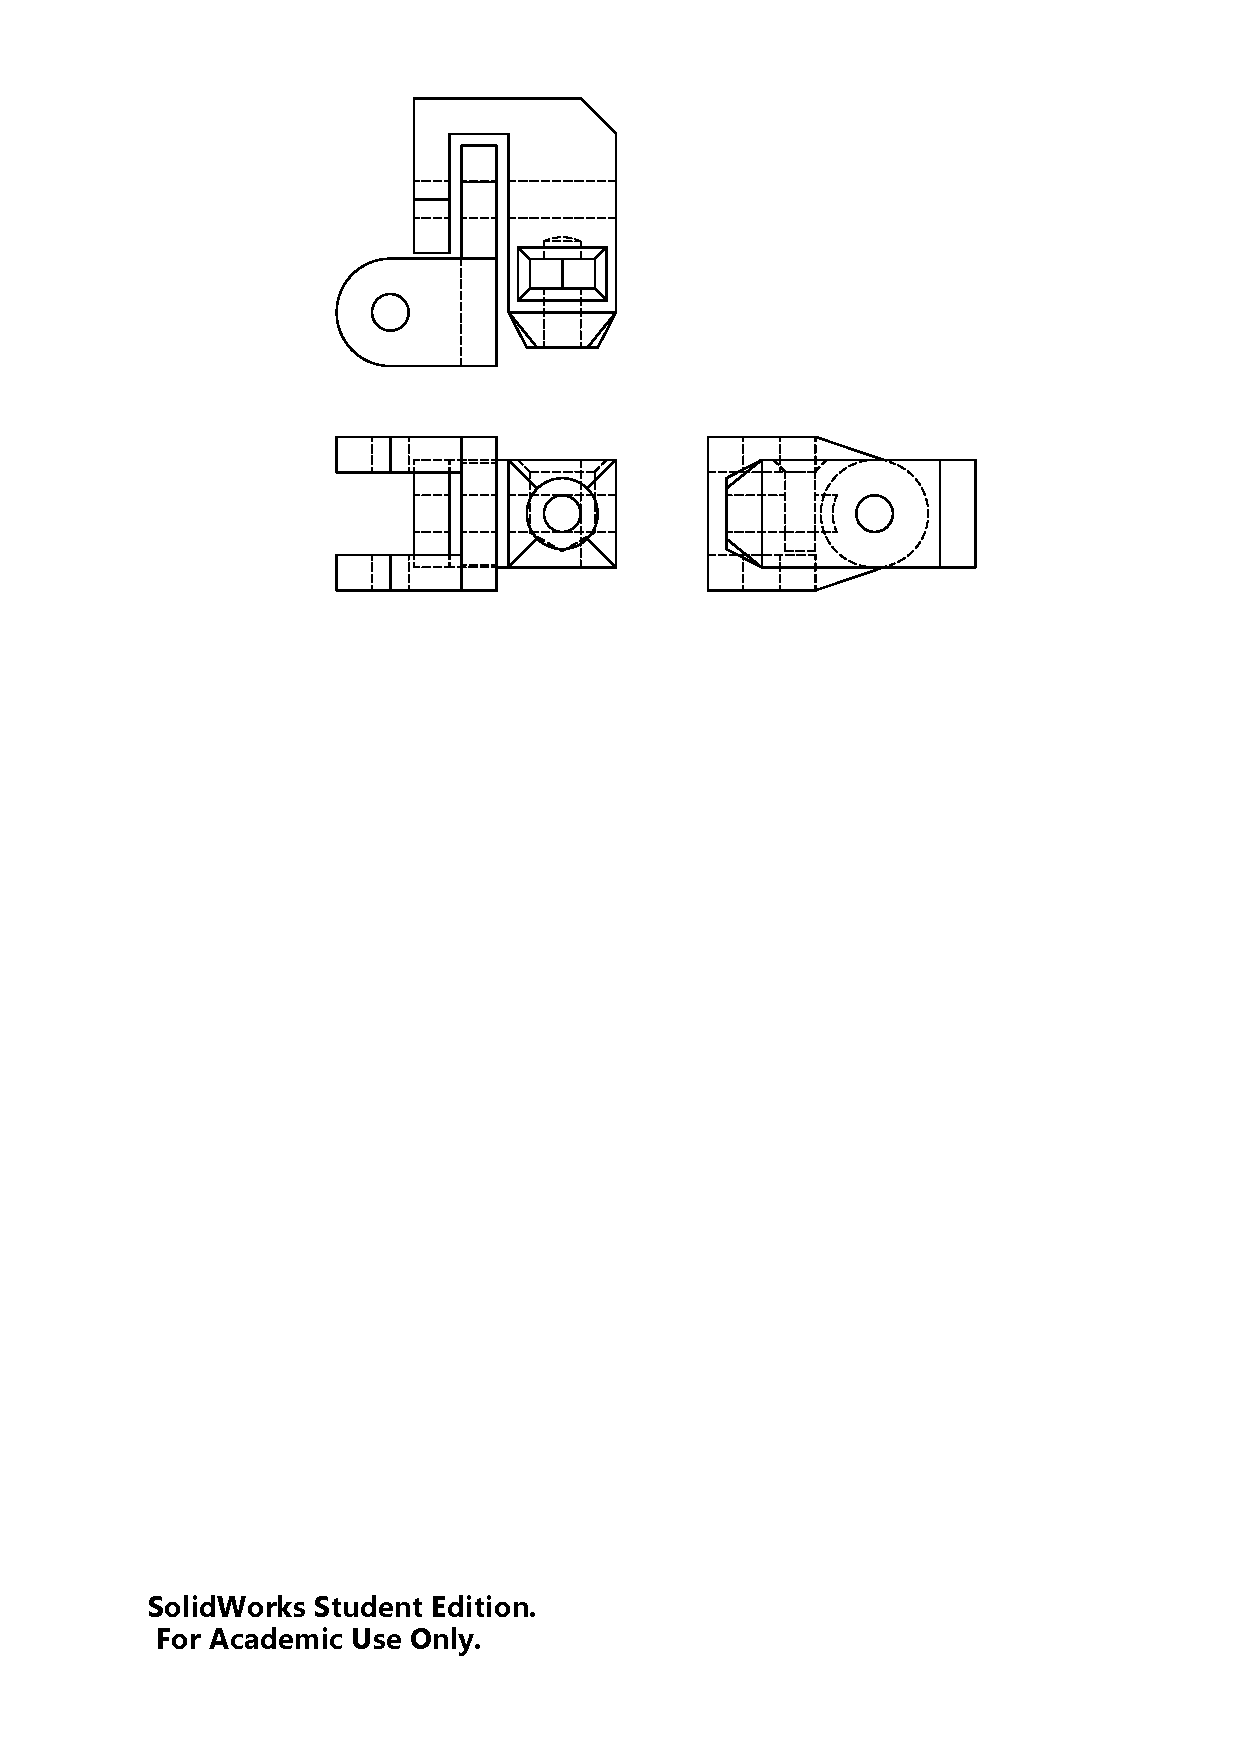
\includegraphics[clip, trim=5cm 18cm 4cm 0cm, width=0.44\linewidth]{figures/two-axis-hinge}
        }%
        \subfloat[]{
          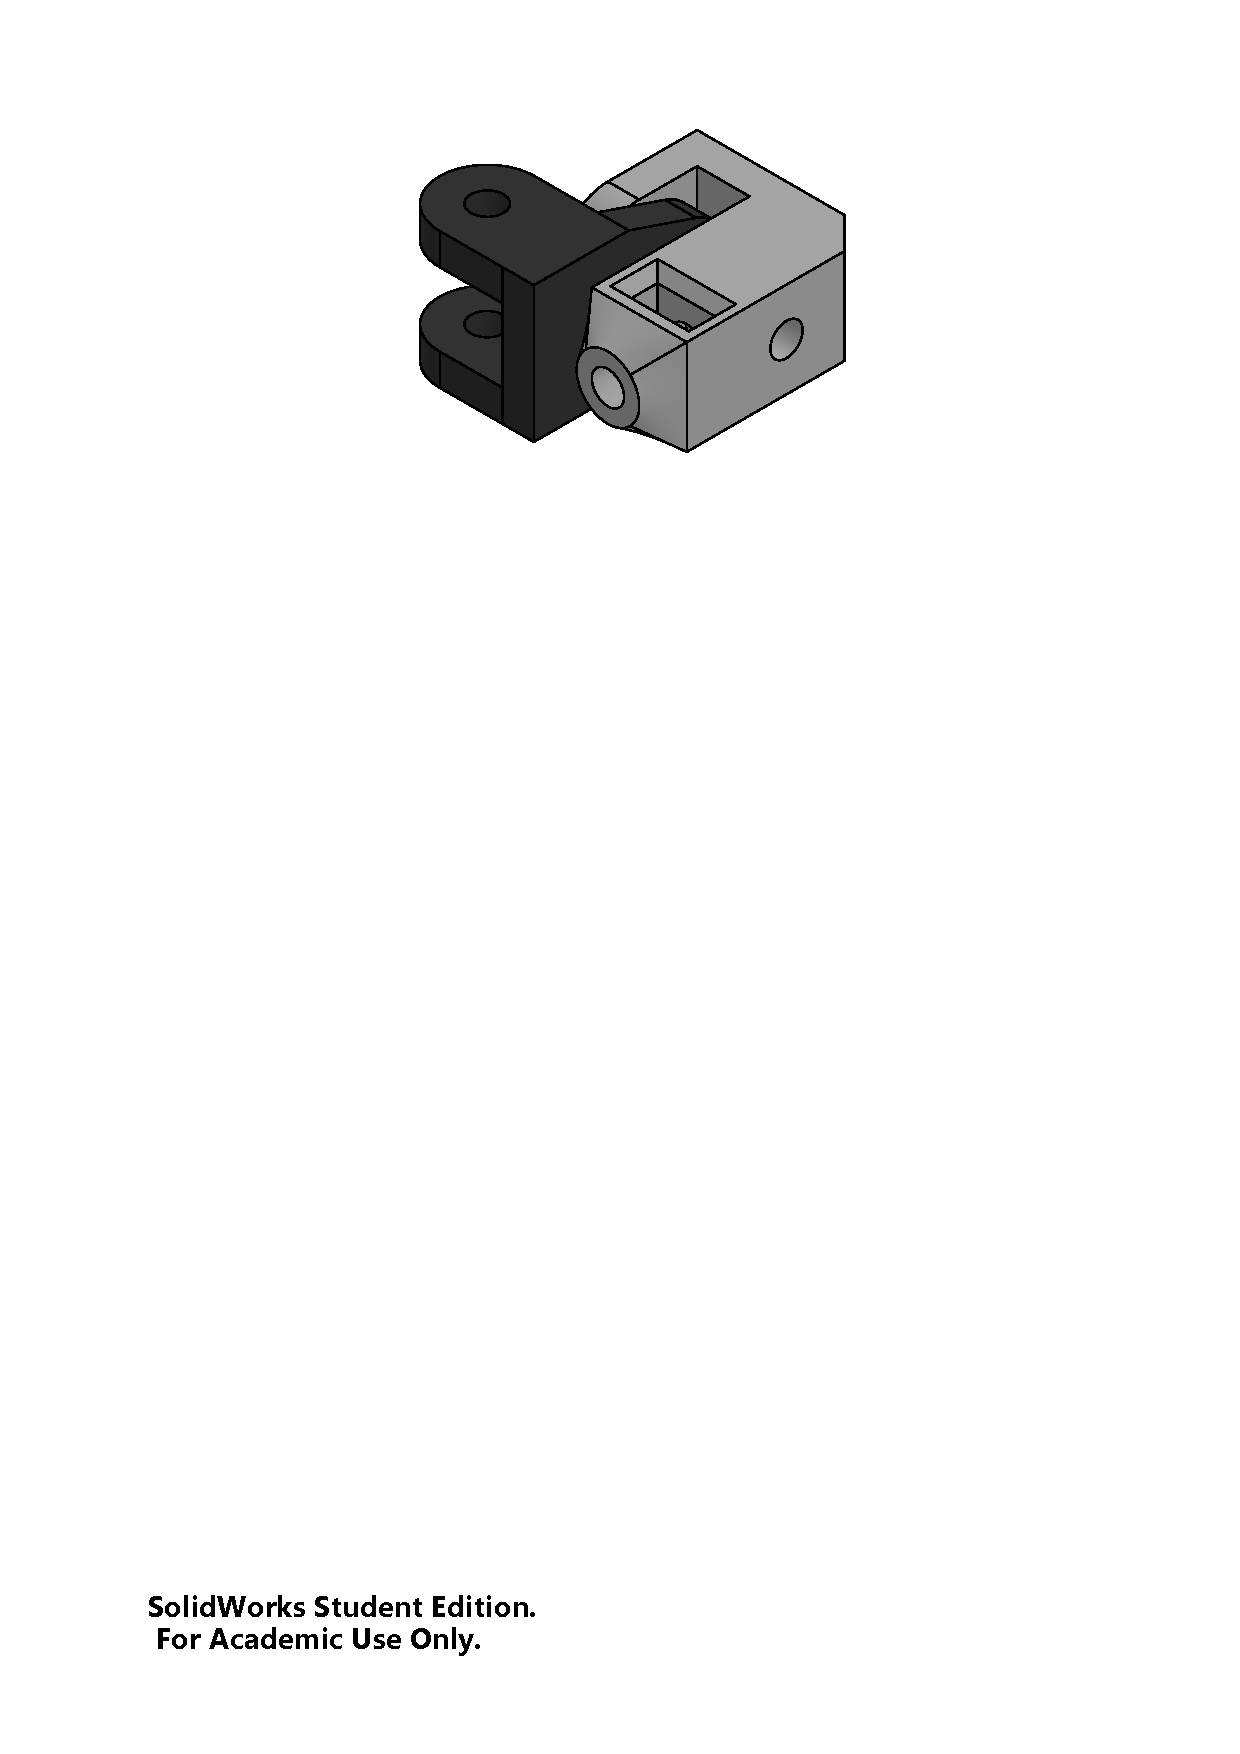
\includegraphics[clip, trim=3cm 19cm 3cm 1cm, width=0.55\linewidth]{figures/two-axis-hinge-iso}
        }
        \caption[Detailed drawings of the two-axis hinge component in the differential system (without fasteners)]{Detailed drawings of the two-axis hinge component in the differential system (without fasteners)}
        \label{fig:mechDesign-twoAxisHingeDetail}
        \end{figure}
        
        It must be noted that other hinge techniques were considered also for this subsystem, one of which included a ball and ring-socket joint which would have provided the required axes of rotation in a single coupling (for each end). The idea was not used for the design due to unavailability of the joints, particularly of the size required. The hinge technique was simpler in design and leant itself well to the chosen manufacture method.
        
      \subheading{Final Sub-assembly}\\\\
        Figure~\ref{fig:mechDesign-differentialSubDetail} shows detail of the differential sub-assembly as generated in the CAD package used and which was analysed for interferences and functional integrity.
        
        \begin{figure}[h!]
        \centering
        \subfloat[\label{fig:mechDesign-differentialSubDetail-a}]{
          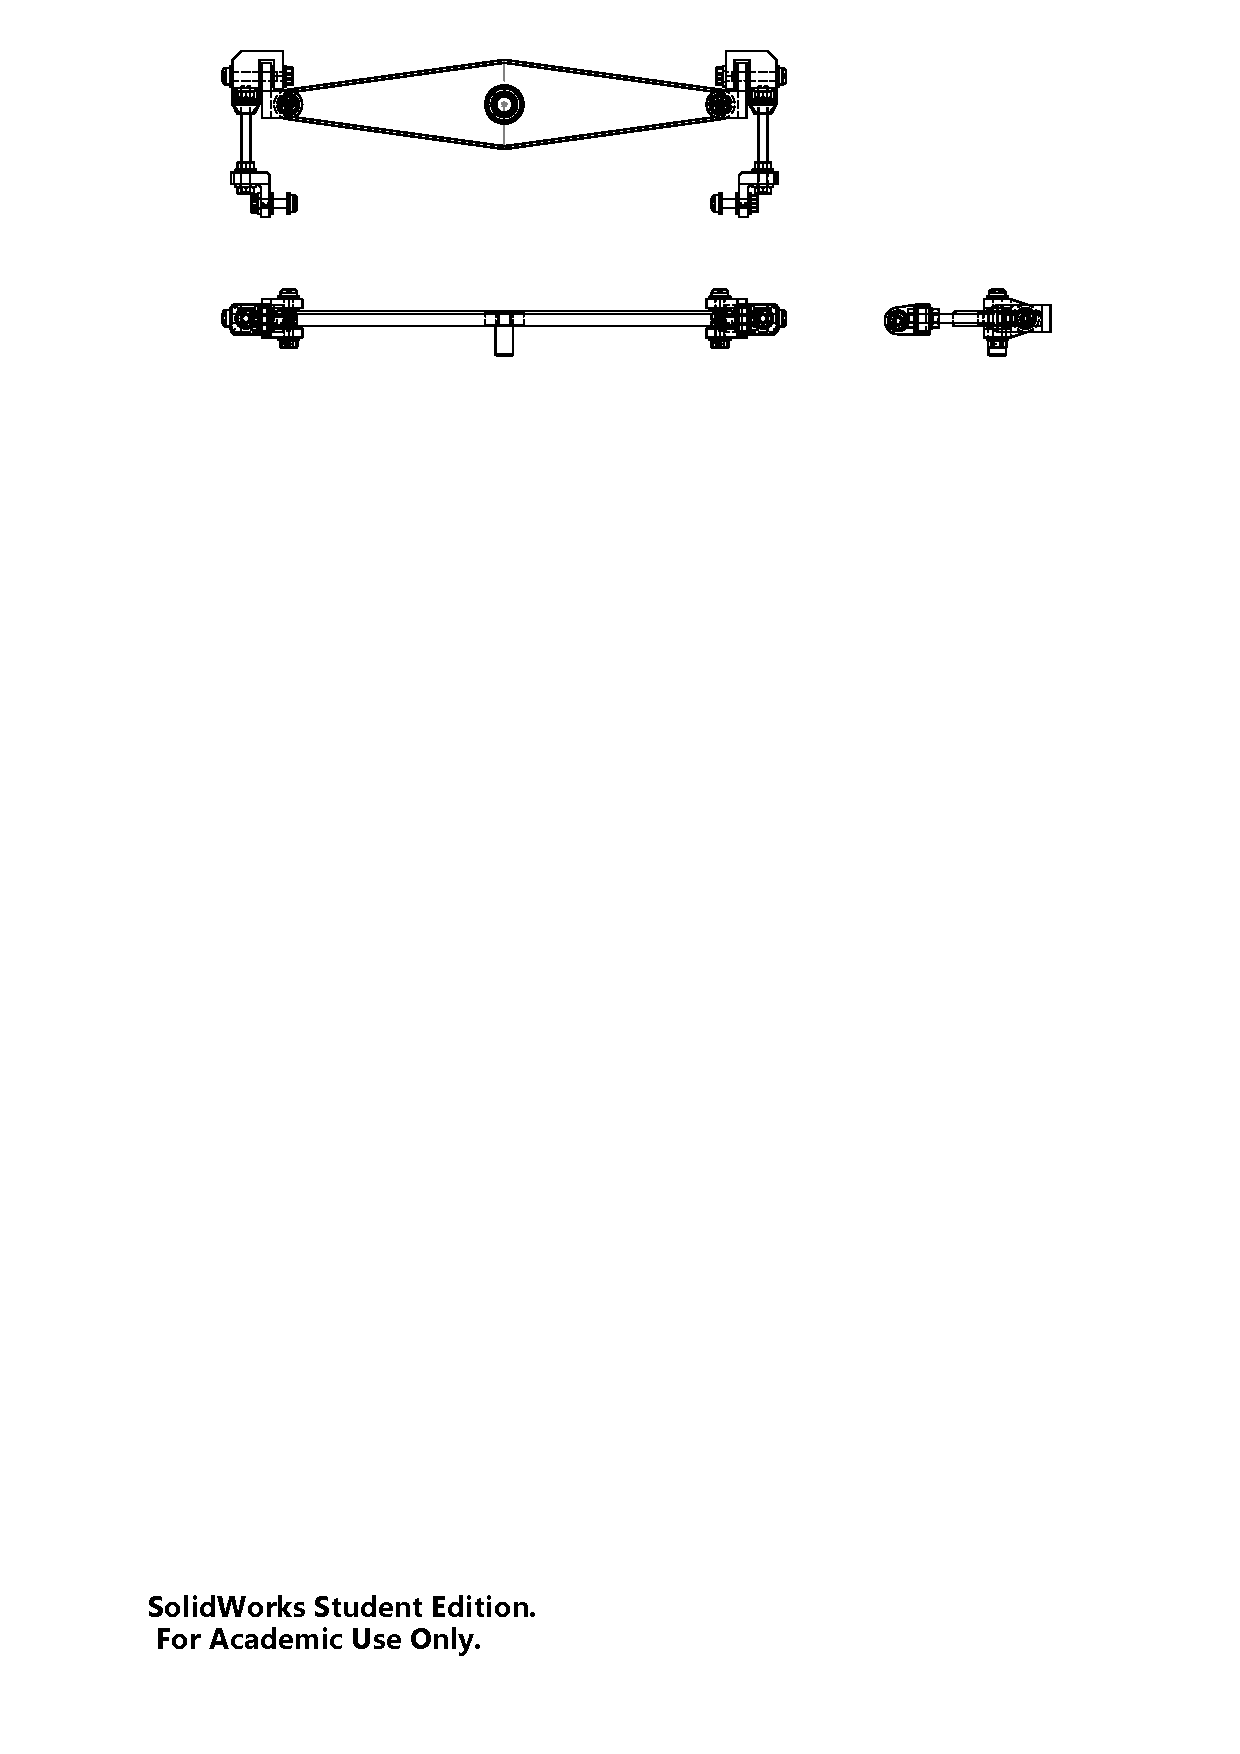
\includegraphics[clip, trim=3cm 22cm 3cm 0cm, width=1\linewidth]{figures/diff-sub}
        }
        \qquad
        \subfloat[\label{fig:mechDesign-differentialSubDetail-b}]{
          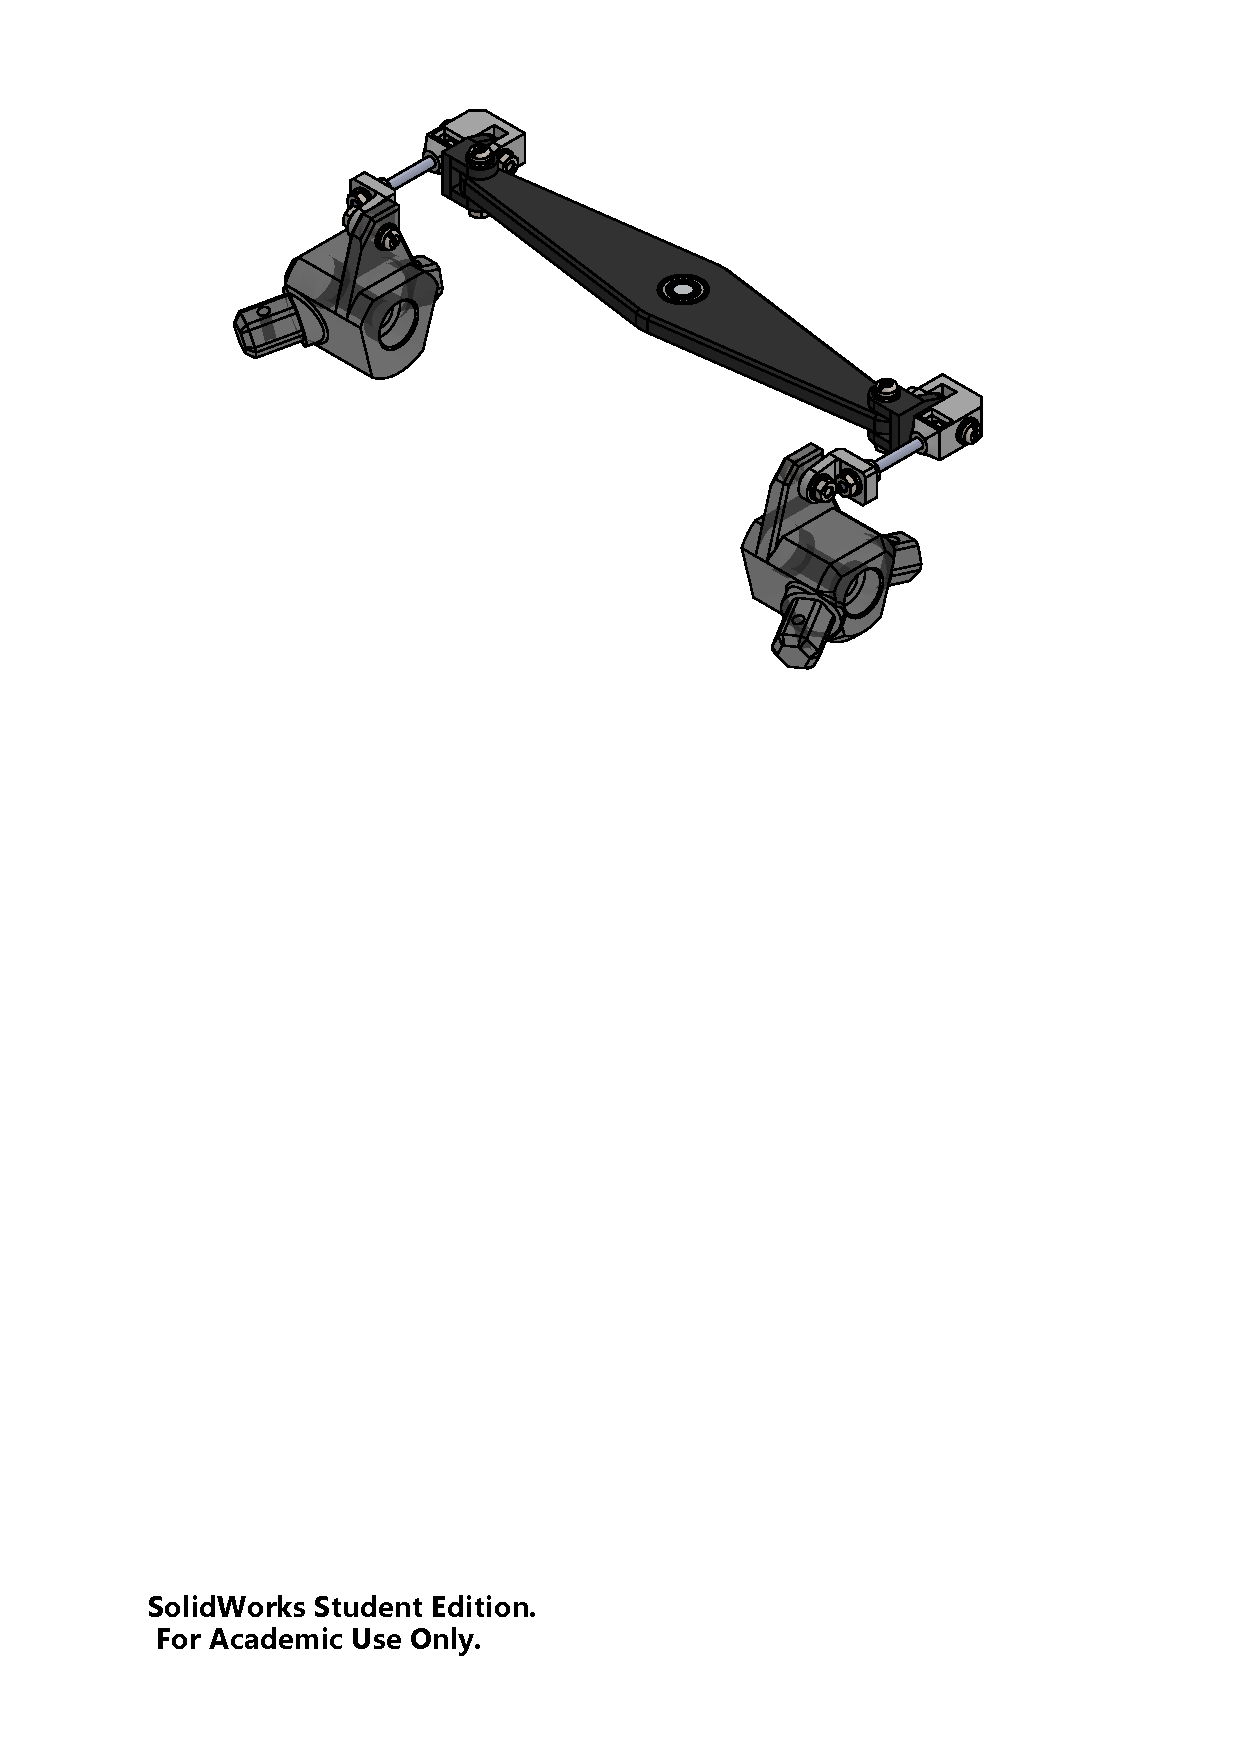
\includegraphics[clip, trim=4cm 17cm 4cm 1cm, width=0.7\linewidth]{figures/diff-sub-iso}
        }
        \caption[Detailed drawings of the working, dynamic assembly of the differential system]{Detailed drawings of the working, dynamic assembly of the differential system (included in the isometric view in \protect\subref{fig:mechDesign-differentialSubDetail-b} are the rocker joints as part of the suspension system)}
        \label{fig:mechDesign-differentialSubDetail}
        \end{figure}
        
              
    \subsubsection{Head and Neck}
      It was decided during the conceptual design phase that both the neck and the head assembly were to be 3D printed and mounted to the top of the rover deck. Since there were two axes of rotation of the head required, as well as at least one piece to facilitate mounting the assembly, three separate components in total were required (a minimum). The assembly also aimed to minimise the amount of movement that components that facilitated mounting of the servos were subjected to for friendlier cable routing. At the same time, the ease of 3D printing such an assembly had an effect on the approach taken when designing the structure and configuration of the components as well as the components themselves. As a result, the configuration designed consisted of a static mount piece, a middle section, referred to as the neck, which allowed mounting of both servos for the two axes of rotation, and a head sub-assembly to mount the camera and the ultrasonic sensor.
      
      \subheading{Neck Mount}\\\\
        The neck mount piece provided the support for the neck and head assembly in its entirety. Besides including holes for mounting to the deck of the rover, the component featured a small blind hole at the top center surface into which the shaft of the pan-axis servo could fit and be fastened to. A smaller hole right through the center allowed the servo shaft screw to be tightened so that the shaft did not spin in its mount.
        
        Figure~\ref{fig:mechDesign-neckMount} shows the detail of the neck mount component.

        \begin{figure}[h!]
        \centering
        \subfloat[]{
          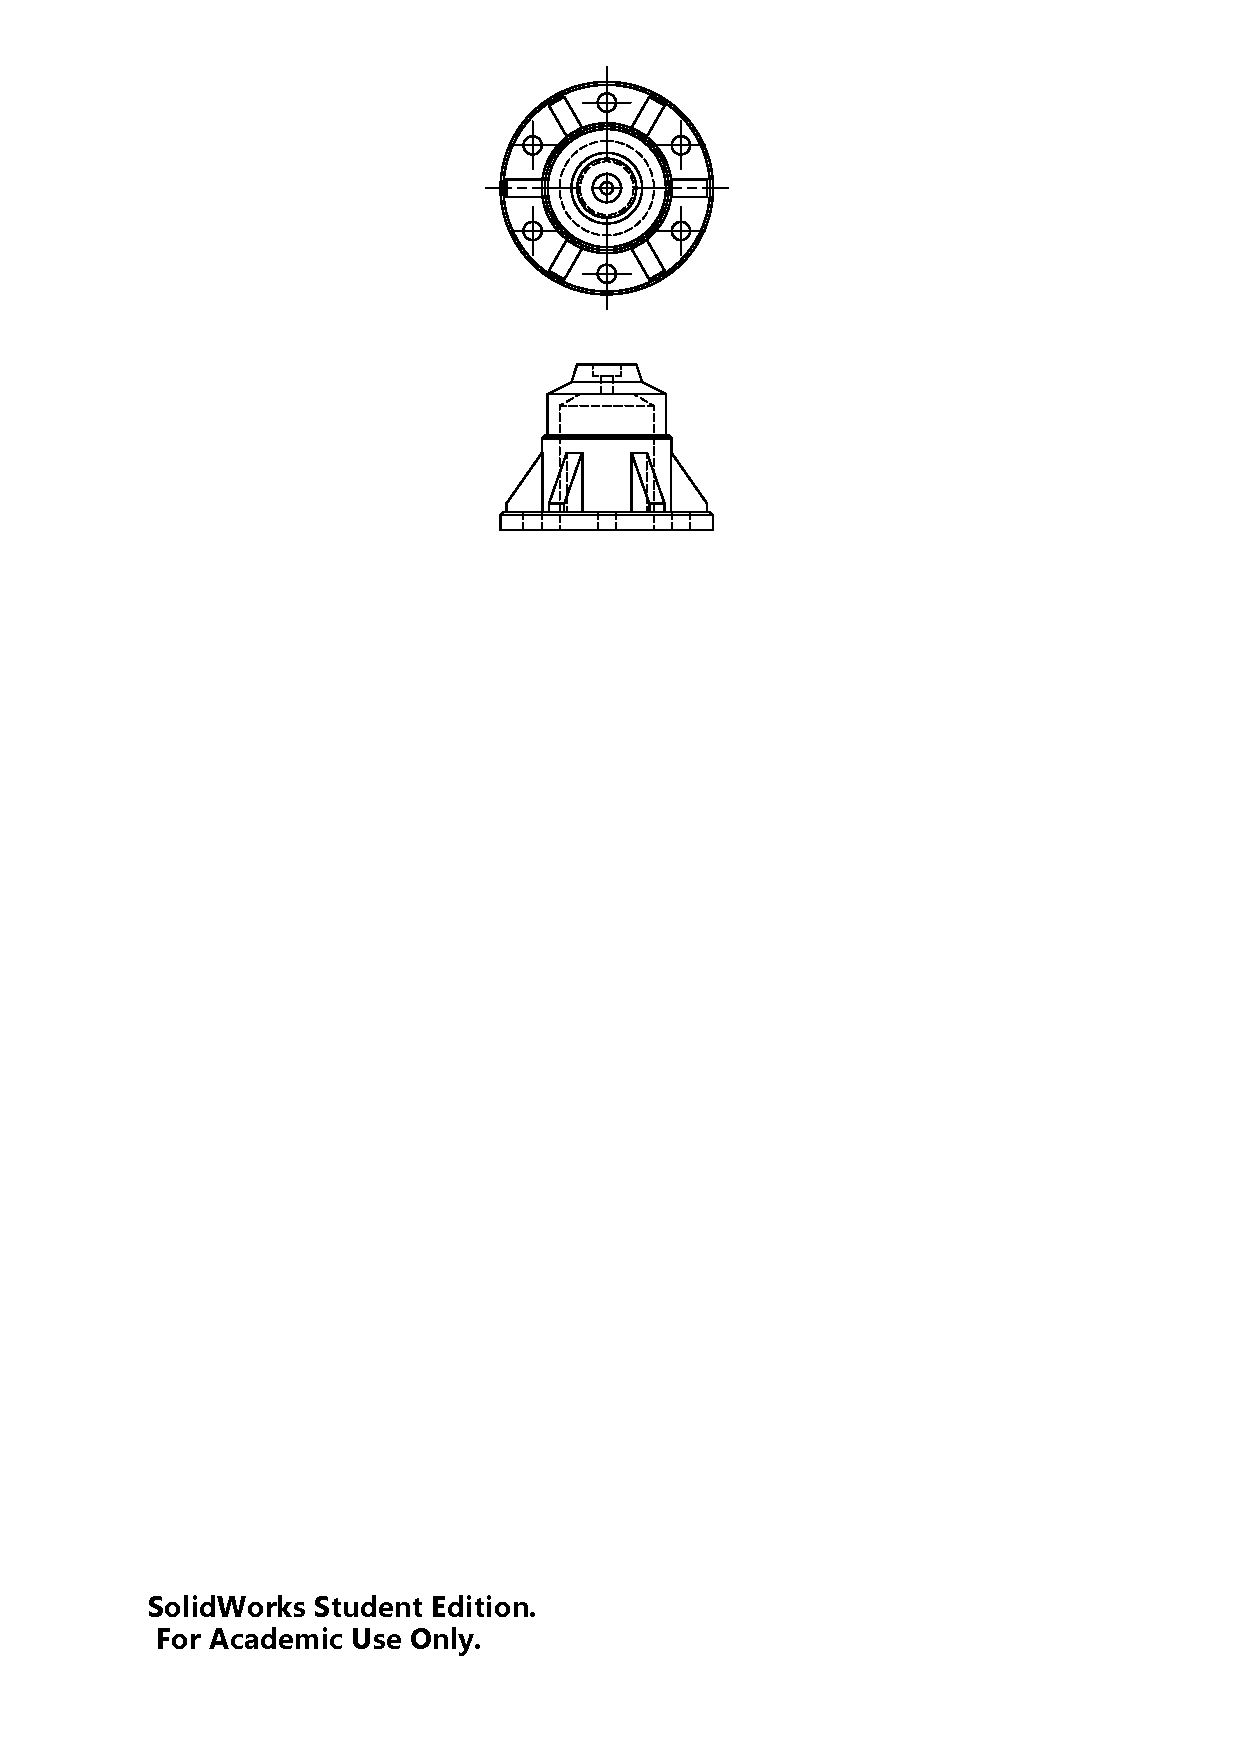
\includegraphics[clip, trim=6cm 19cm 6cm 0cm, width=0.49\linewidth]{figures/mastMount-top}
        }%
        \subfloat[]{
          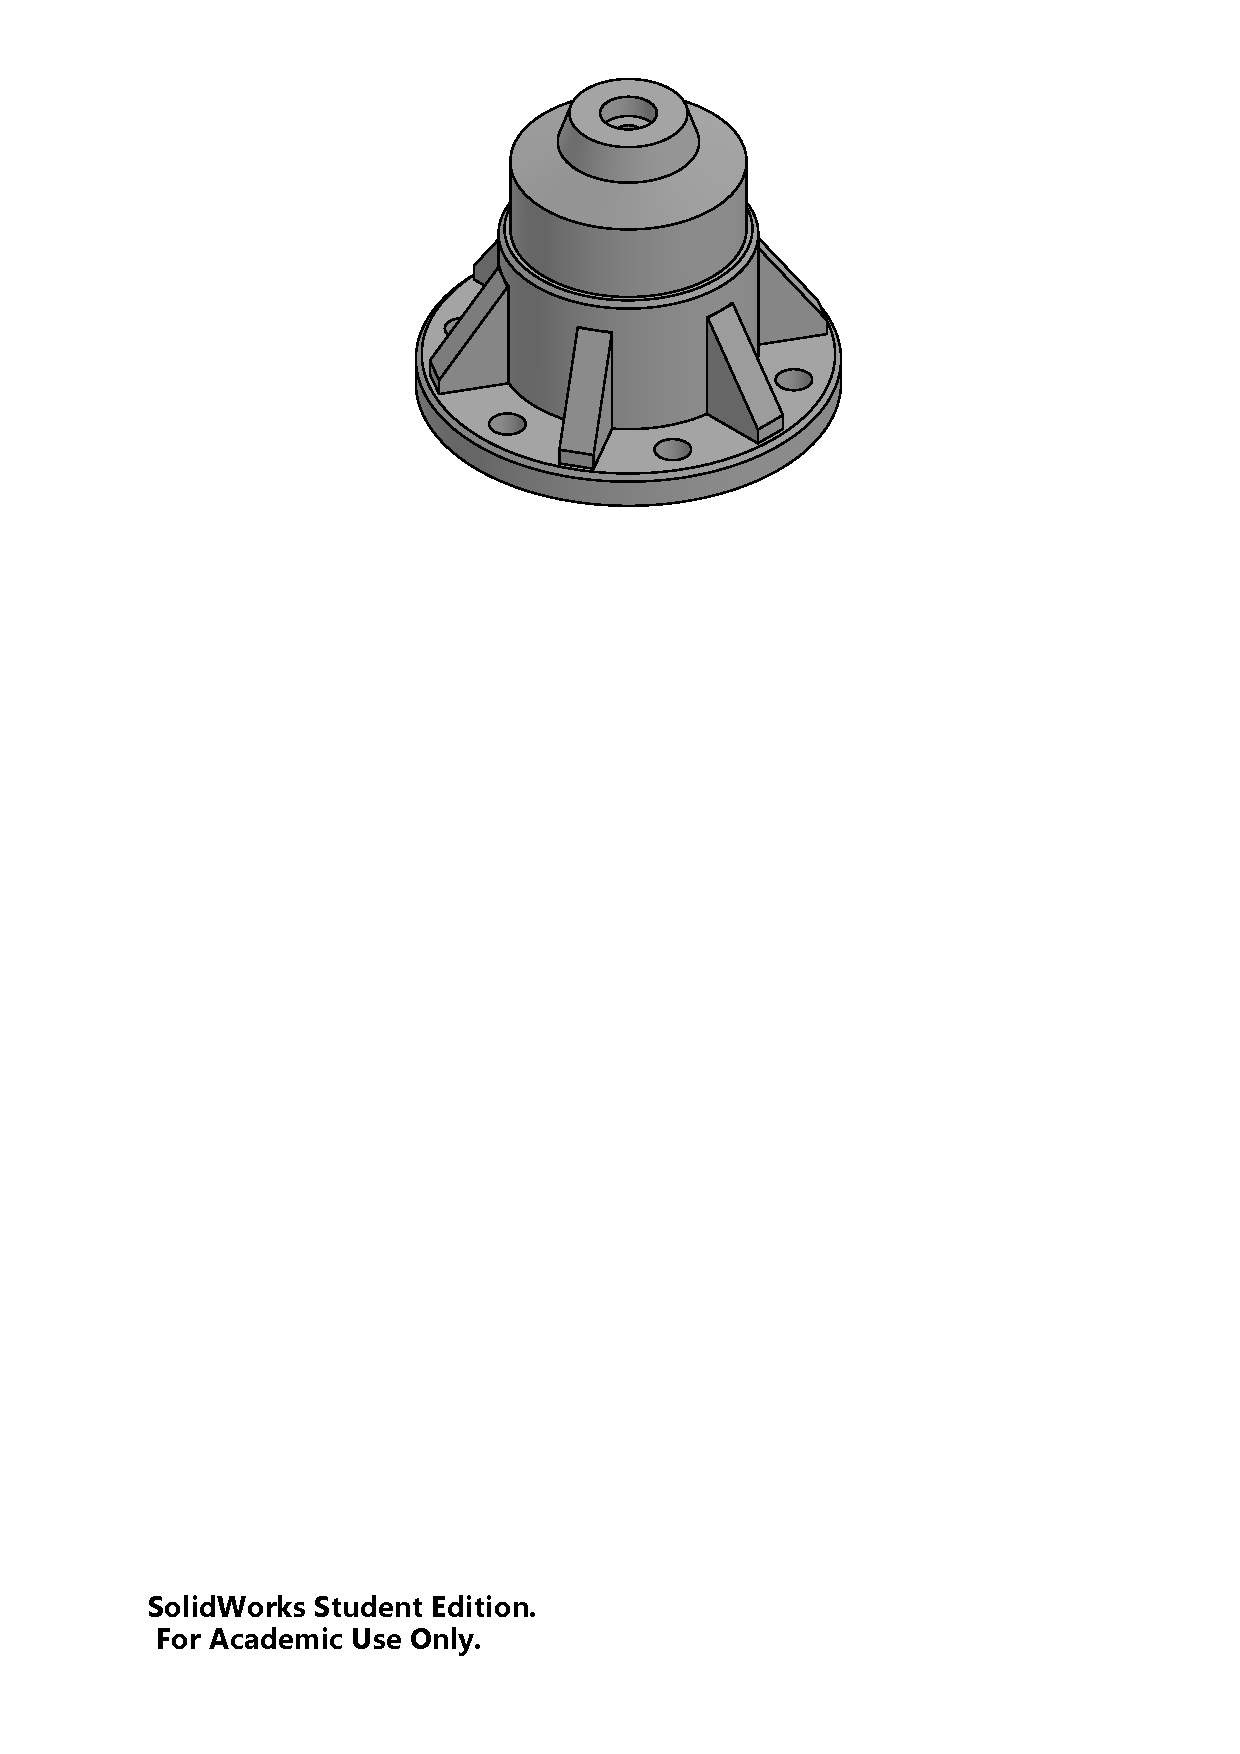
\includegraphics[clip, trim=3cm 17cm 3cm 1cm, width=0.49\linewidth]{figures/mastMount-top-iso}
        }
        \caption[Detailed drawings of the neck mount component in the head and neck sub-assembly]{Detailed drawings of the neck mount component in the head and neck sub-assembly}
        \label{fig:mechDesign-neckMount}
        \end{figure}

      \subheading{Neck Hinge and Actuation}\\\\
        The center piece in the neck-head assembly, referred to as the neck hinge, was designed to facilitate the mounting of two servos: one for pan movement and the other for pitch movement. As discussed, the pan-axis, servo which by definition was facing downwards towards the rover deck surface, would fit into hole in the top of the neck mount and support the rest of the neck-head assembly. Fitted into the neck hinge component was the pitch-axis servo which was displaced from the pan-axis servo by 90 degrees. Multiple configurations involving the placement of the servos were considered and the one which had the smallest volumetric footprint as well as required the least amount of 3D printing material was chosen. This configuration had the servos positioned flat against each other with support material positioned at the servo mounting holes, the assembly of which can be seen in Figure~\ref{fig:mechDesign-neckHingeServoSubExpl}. Figure~\ref{fig:mechDesign-neckHinge} shows the detailed drawing of the neck hinge component without the servos.
        
        \begin{figure}[h!]
        \centering
        \subfloat[]{
          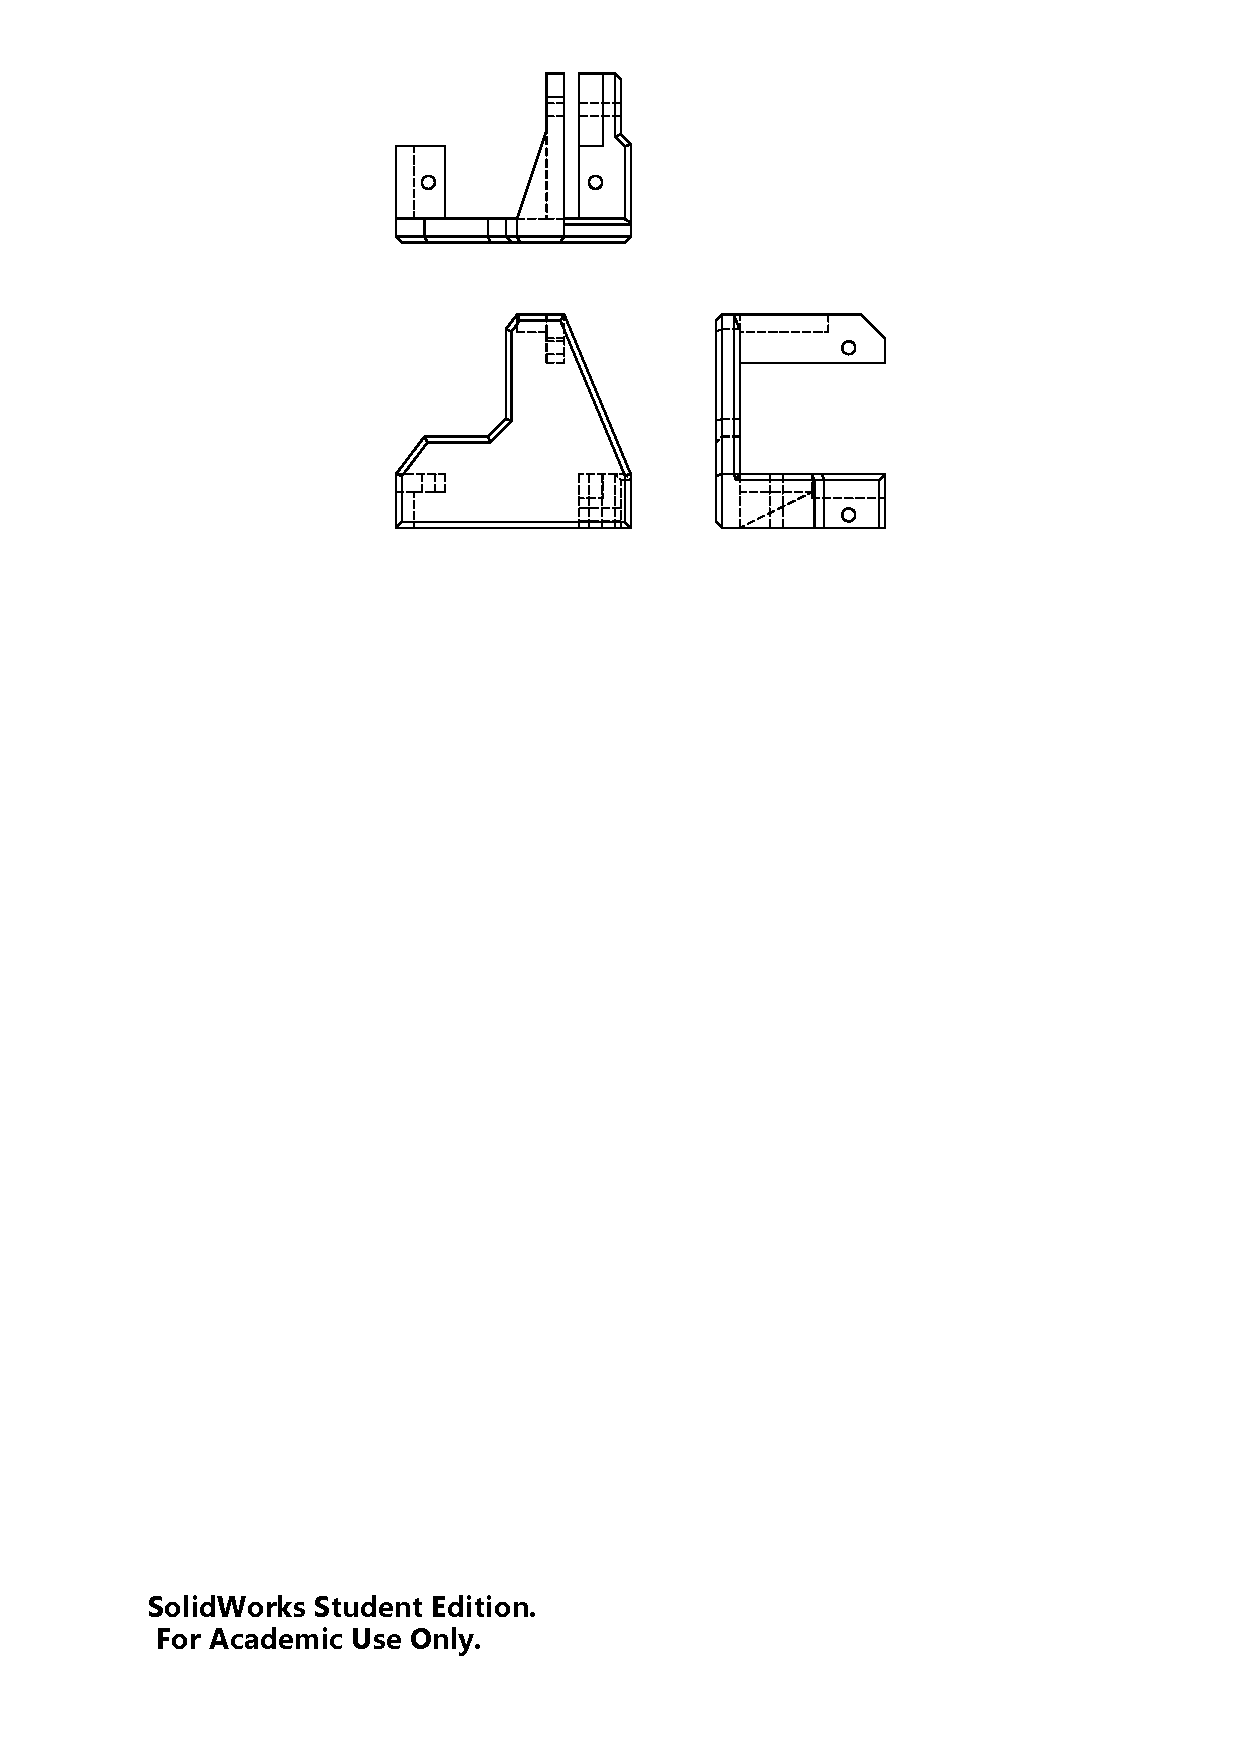
\includegraphics[clip, trim=6cm 19cm 6cm 0cm, width=0.44\linewidth]{figures/neck-hinge}
        }%
        \subfloat[]{
          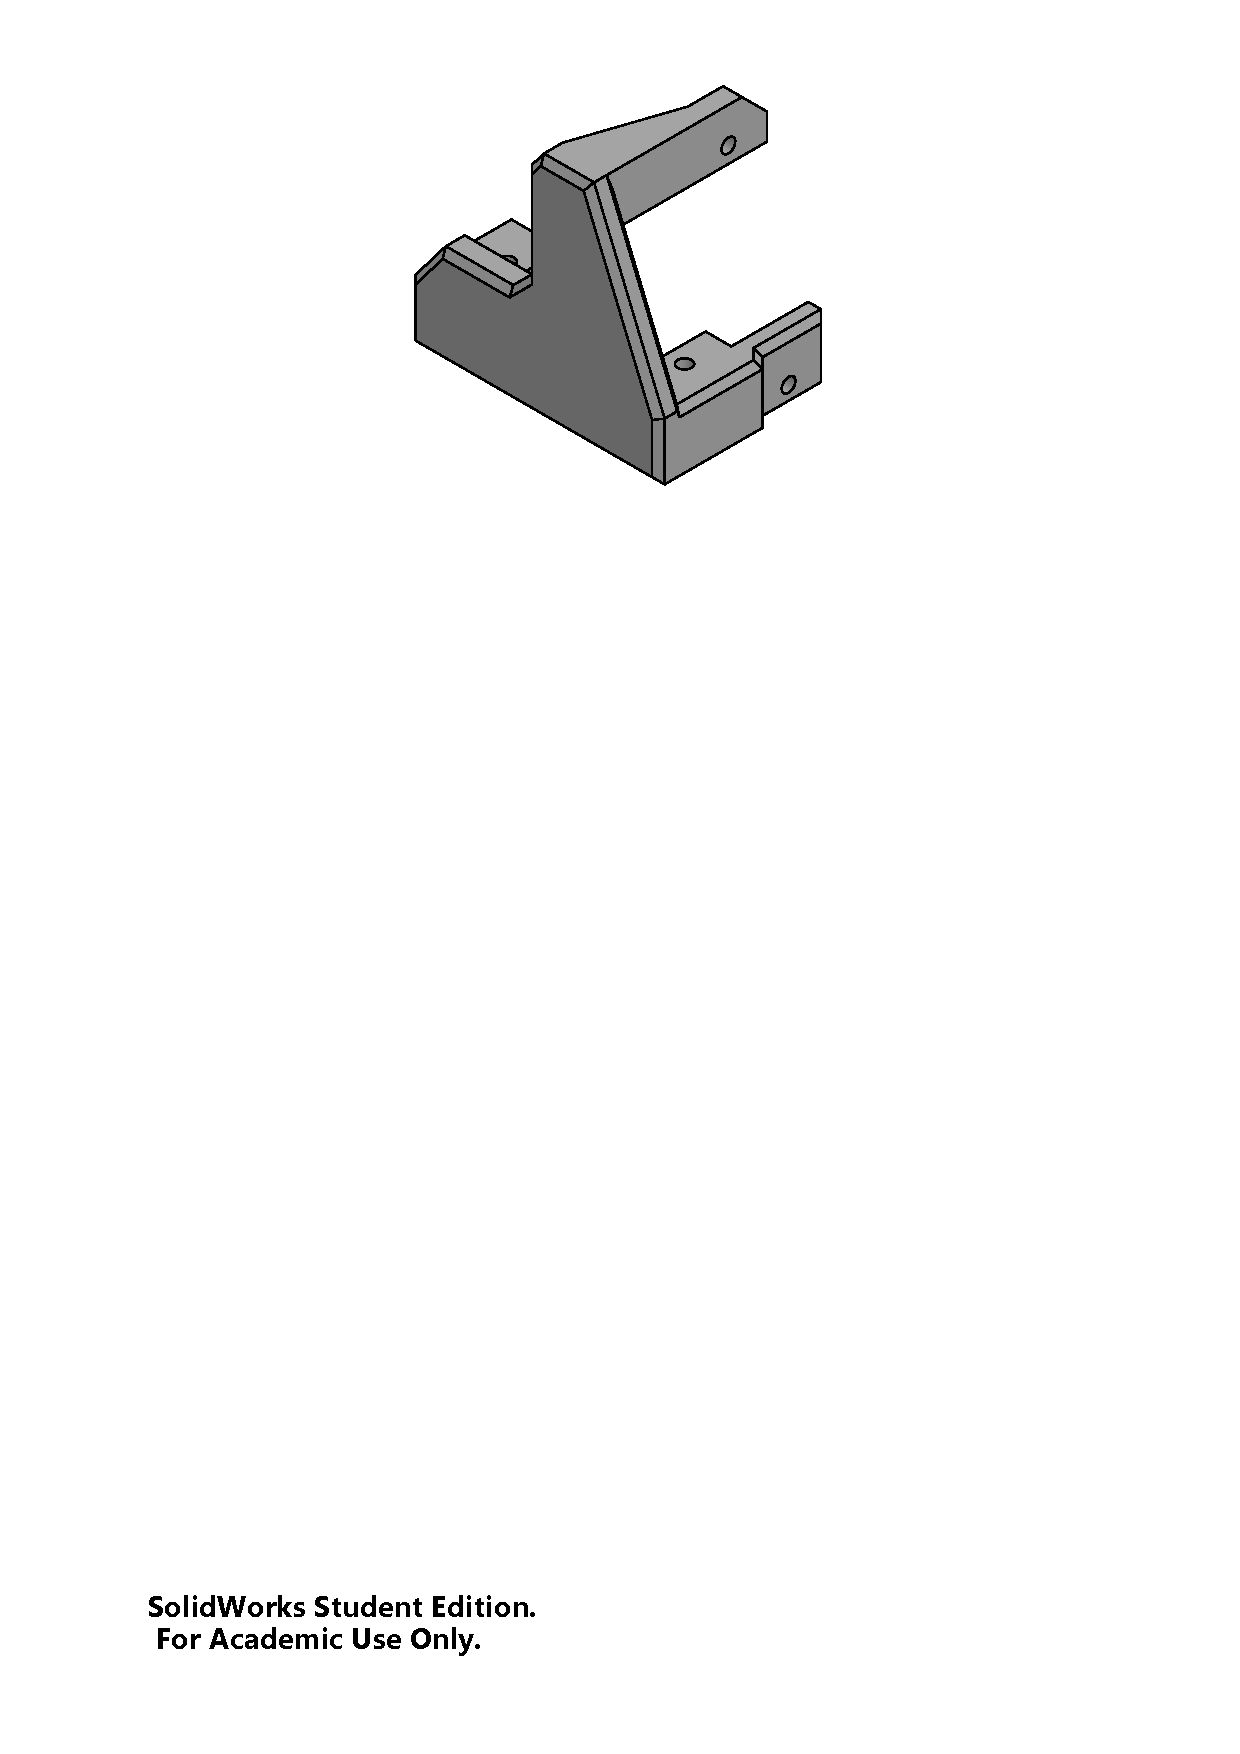
\includegraphics[clip, trim=4cm 18cm 4cm 1cm, width=0.55\linewidth]{figures/neck-hinge-iso}
        }
        \caption[Detailed drawings of the neck hinge component in the head and neck sub-assembly]{Detailed drawings of the neck hinge component in the head and neck sub-assembly}
        \label{fig:mechDesign-neckHinge}
        \end{figure}
        
        \begin{figure}[h!]
          \centering
          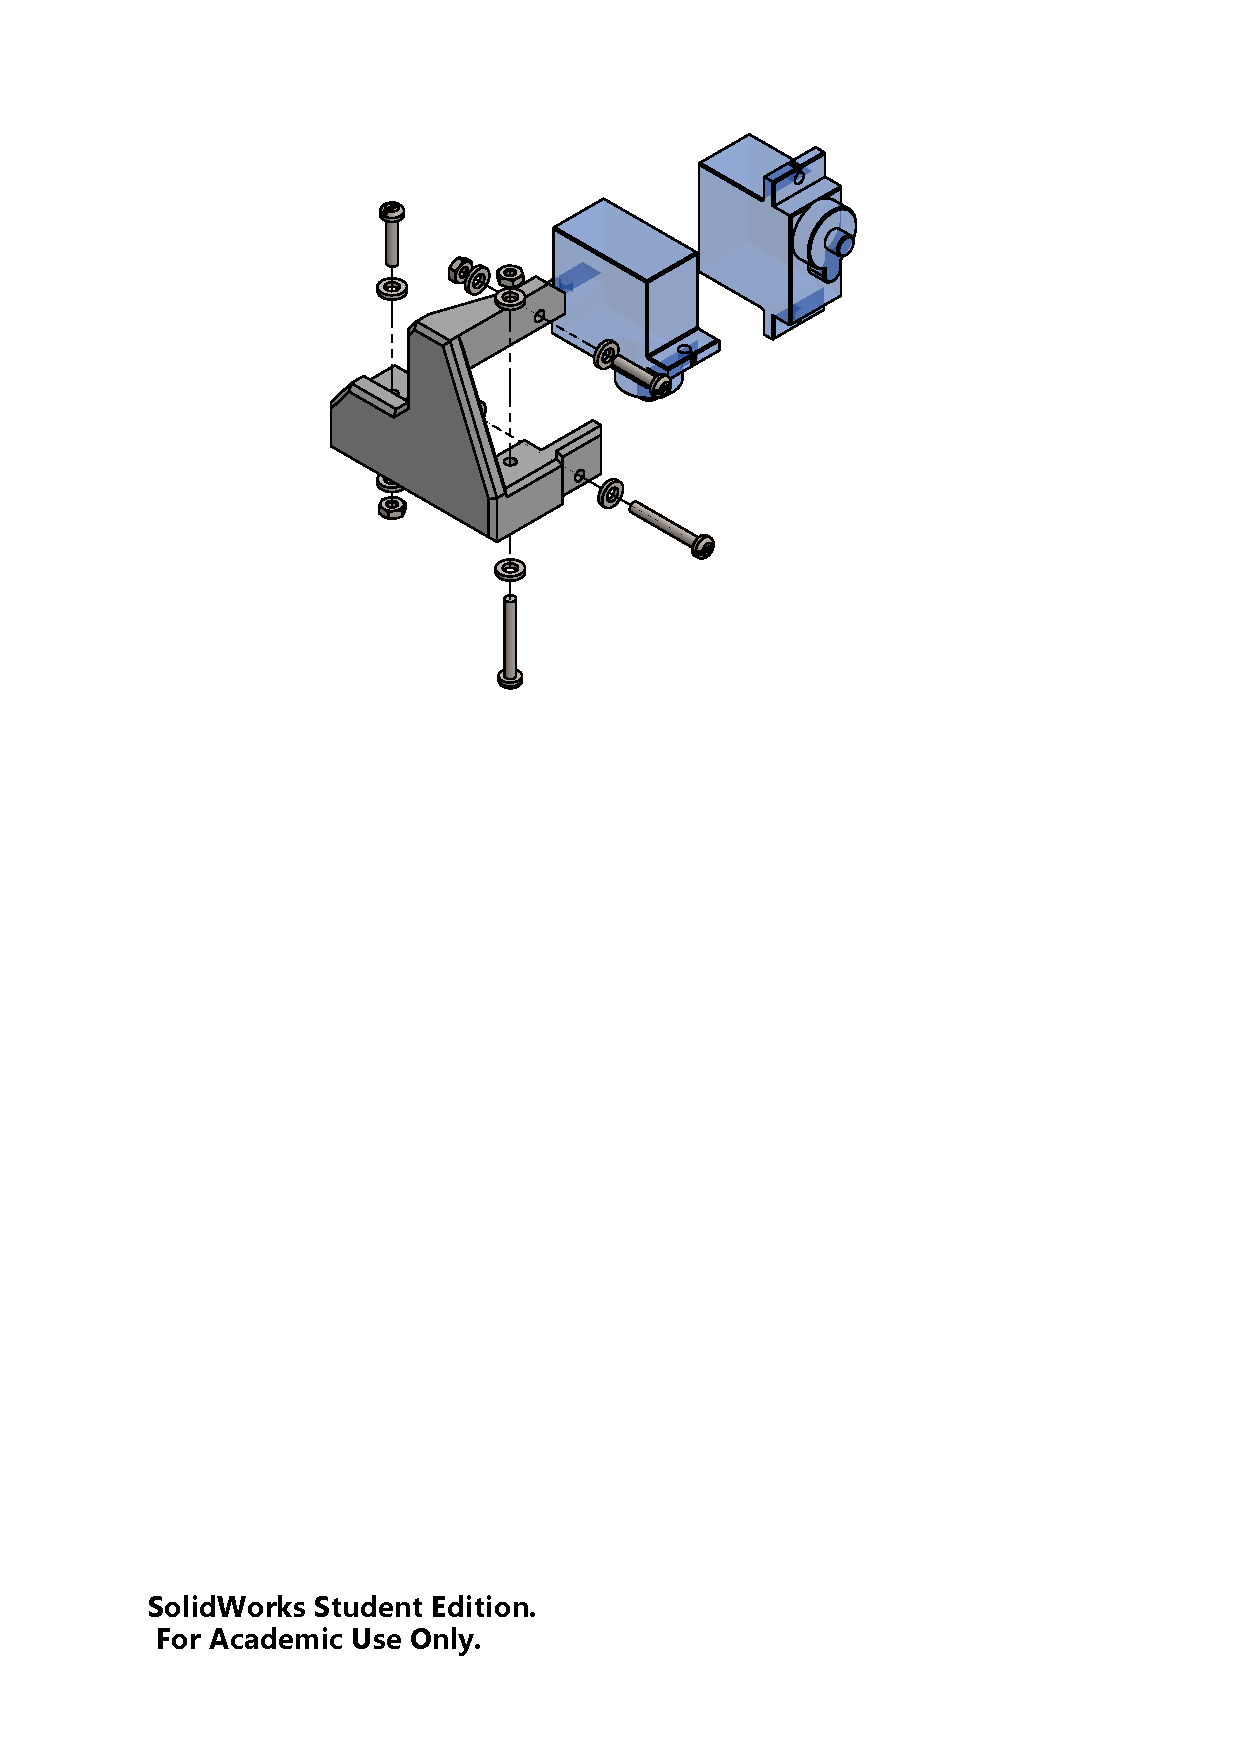
\includegraphics[clip, trim=3cm 17cm 3cm 1cm, width=1\linewidth]{figures/neck-hinge-servo-sub-expl}
          \caption[Exploded isometric view of the neck hinge and servo assembly]{Exploded isometric view of the neck hinge and servo assembly}
          \label{fig:mechDesign-neckHingeServoSubExpl}
        \end{figure}

      \subheading{Head}\\\\
        The head sub-assembly provided an enclosure for the web camera as well as a surface onto which the head ultrasonic sensor was mounted. As mentioned, the very least number of components required for the two-degrees-of-freedom assembly was three, however, the head sub-assembly required two additional pieces. These components were added to reduce the complexity of the components and therefore improve on 3D printing time and material use.
        
        The head enclosure consisted of two components: a flat base and a box-like canopy. The canopy included an arched cut-out which allowed the camera, mounted on the inside, to view the outside world. The canopy was designed as a separate piece so that it could be removed to install and access the camera. As a minimisation of the footprint required by the fastening of the canopy to the base component, inset neodymium magnets were placed at all four corners of the canopy and base components such that the canopy clicked onto the base. Additionally, the canopy was designed to resemble as closely as possible the head on \textit{Curiosity} as this was one of the rover's more recognisable and characteristic components from an aesthetic perspective.
        
        The second extra piece included in the head sub-assembly was a right-angled bracket designed to be mounted to the shaft of the pitch-axis servo using a cross-shaped servo horn and fastened to the bottom of the head base component.
        
        Figures~\ref{fig:mechDesign-headBasePlate}, \ref{fig:mechDesign-headCanopy} and \ref{fig:mechDesign-headRightBracket} show detailed views of the three head components.

        \begin{figure}[h!]
        \centering
        \subfloat[]{
          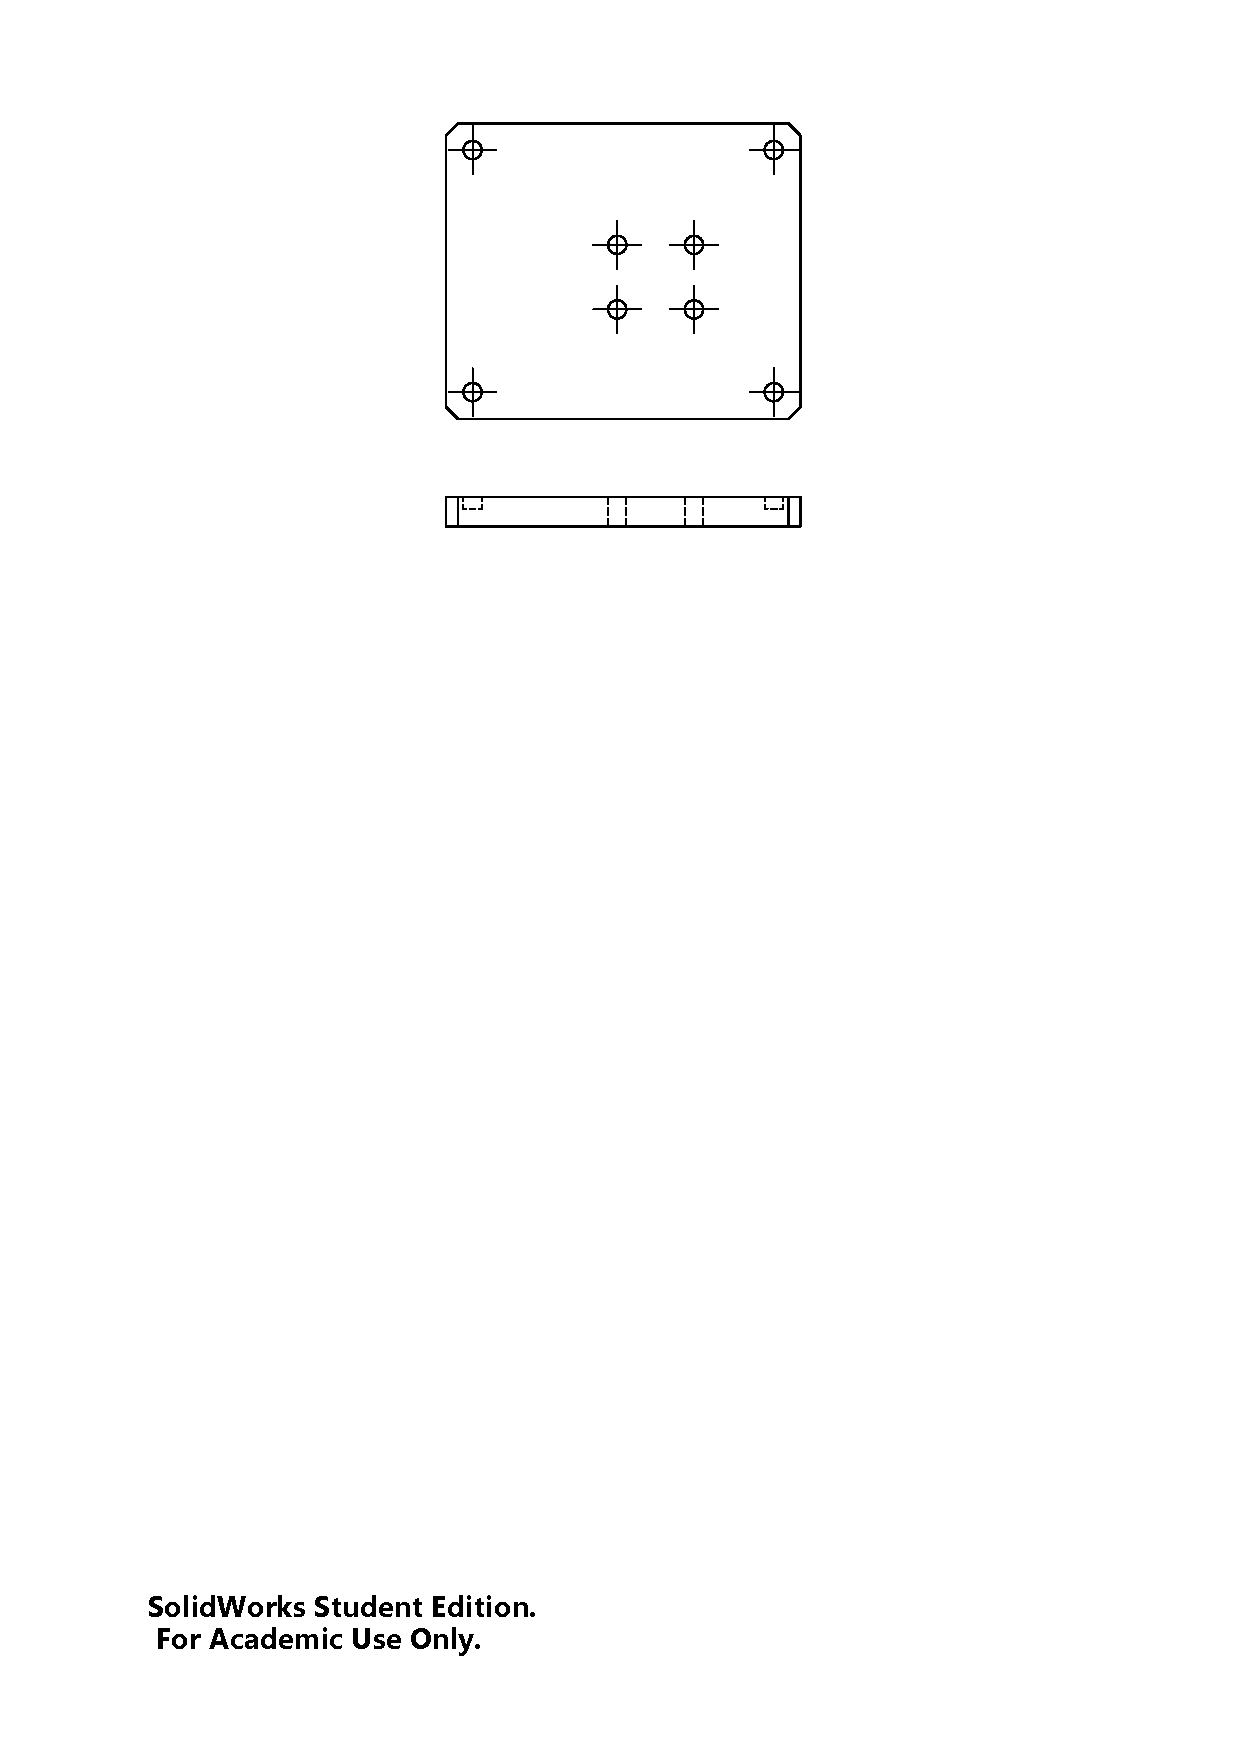
\includegraphics[clip, trim=6cm 19cm 6cm 0cm, width=0.44\linewidth]{figures/headBaseplate}
        }%
        \subfloat[]{
          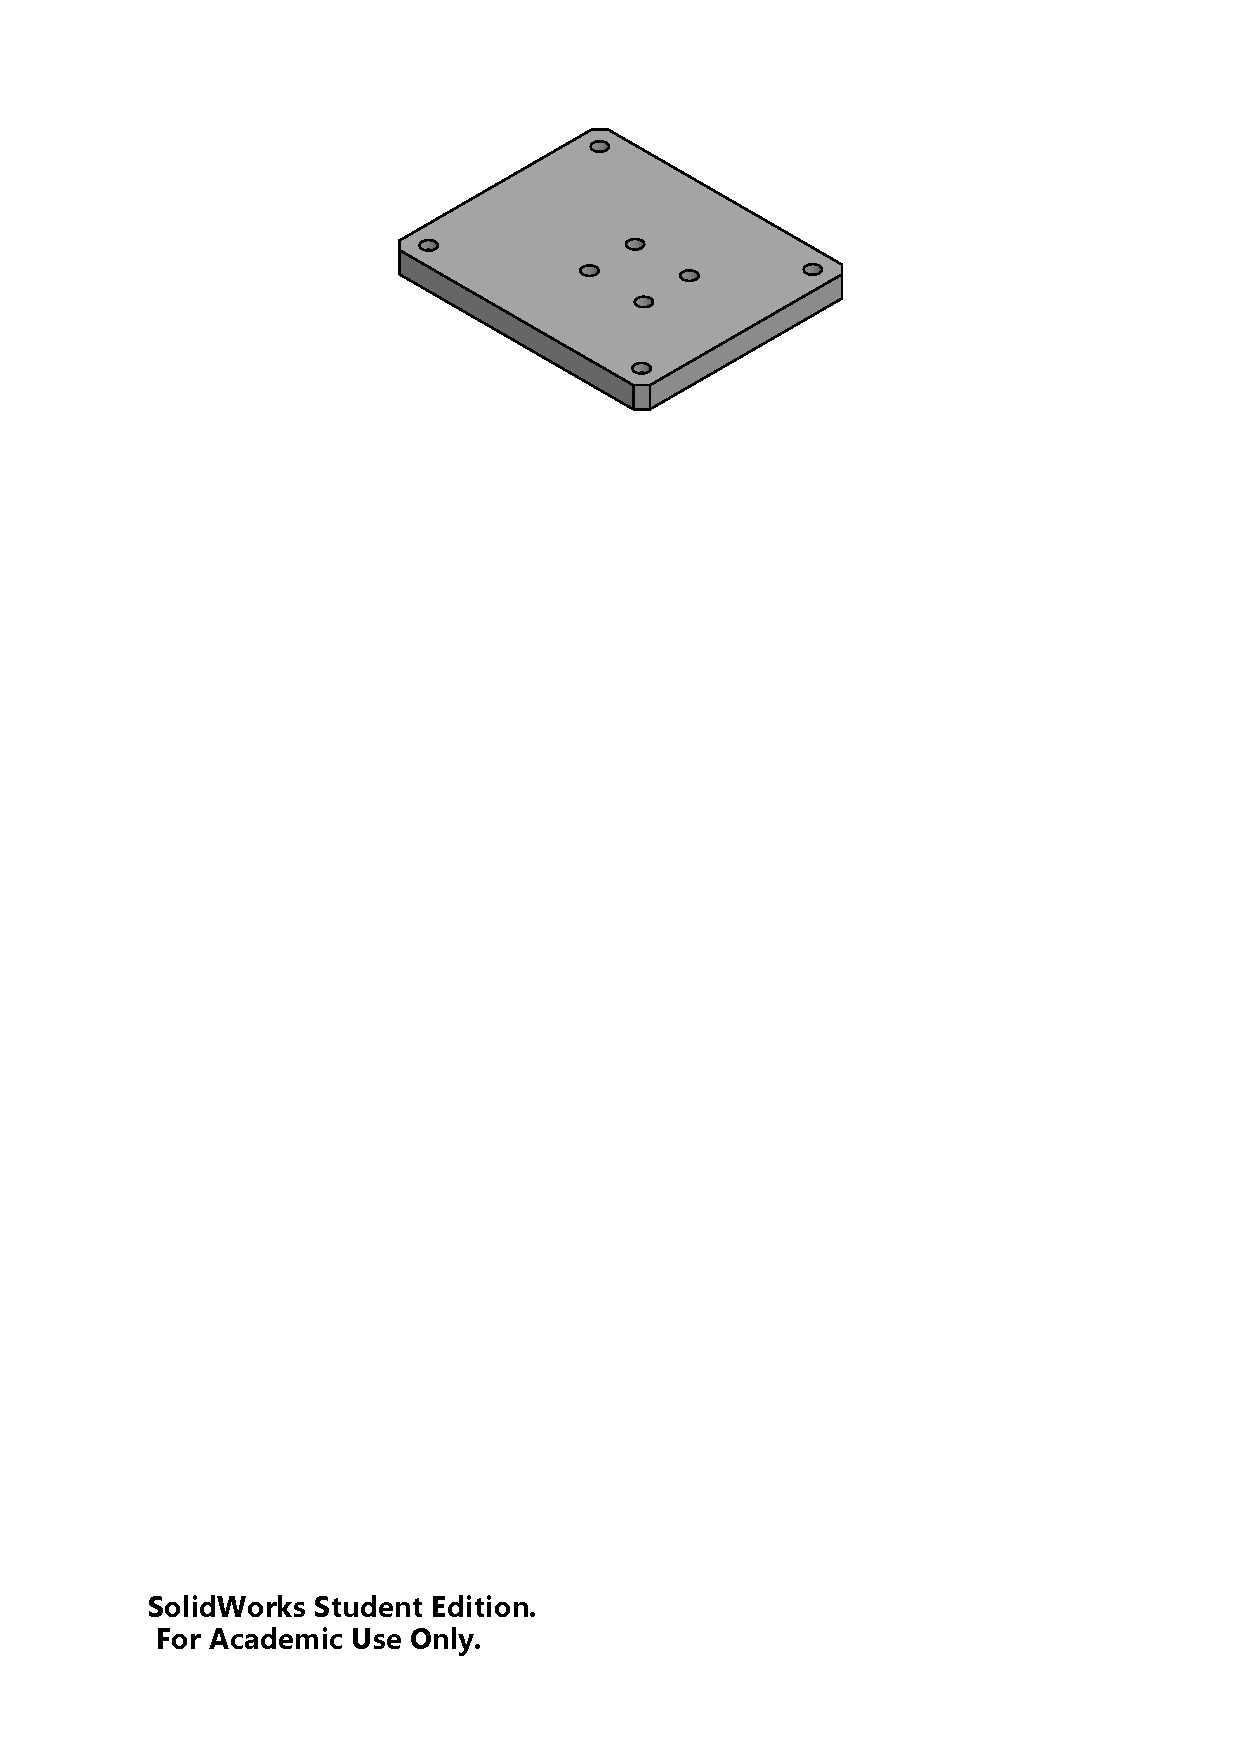
\includegraphics[clip, trim=4cm 18cm 4cm 1cm, width=0.55\linewidth]{figures/headBaseplate-iso}
        }
        \caption[Detailed drawings of the head base component in the head and neck sub-assembly]{Detailed drawings of the head base component in the head and neck sub-assembly}
        \label{fig:mechDesign-headBasePlate}
        \end{figure}

        \begin{figure}[h!]
        \centering
        \subfloat[]{
          \includegraphics[clip, trim=6cm 19cm 6cm 0cm, width=0.44\linewidth]{figures/head-canopy}
        }%
        \subfloat[]{
          \includegraphics[clip, trim=4cm 18cm 4cm 1cm, width=0.55\linewidth]{figures/head-canopy-iso}
        }
        \caption[Detailed drawings of the head canopy component in the head and neck sub-assembly]{Detailed drawings of the head canopy component in the head and neck sub-assembly}
        \label{fig:mechDesign-headCanopy}
        \end{figure}

        \begin{figure}[h!]
        \centering
        \subfloat[]{
          \includegraphics[clip, trim=6cm 19cm 6cm 0cm, width=0.44\linewidth]{figures/right-bracket}
        }%
        \subfloat[]{
          \includegraphics[clip, trim=4cm 18cm 4cm 1cm, width=0.55\linewidth]{figures/right-bracket-iso}
        }
        \caption[Detailed drawings of the right bracket component in the head and neck sub-assembly]{Detailed drawings of the right bracket component in the head and neck sub-assembly}
        \label{fig:mechDesign-headRightBracket}
        \end{figure}

      \subheading{Final Sub-assembly}\\\\
        The final sub-assembly of the neck and head components, including the servos is shown in Figure~\ref{fig:mechDesign-headSubDetail}.
        
        \begin{figure}[h!]
        \centering
        \subfloat[]{
          \includegraphics[clip, trim=3cm 18cm 3cm 1cm, width=0.7\linewidth]{figures/headSub}
        }
        \qquad
        \subfloat[]{
          \includegraphics[clip, trim=4cm 17cm 4cm 1cm, width=0.7\linewidth]{figures/headSub-iso}
        }
        \caption[Detailed drawings of the working, dynamic assembly of the head and neck system]{Detailed drawings of the working, dynamic assembly of the head and neck system}
        \label{fig:mechDesign-headSubDetail}
        \end{figure}
        
    \subsubsection{Body}
      The body was a significant part of the rover, designed as a mounting platform for most of the rover's other mechanical and electronic components. The conceptual analysis of the proposed ideas for the assembly of the body settled on the use of acrylic sheet. The body was rectangularly box-shaped and, for the purpose of access to the electronics which were to be mounted internally, the bottom was left open. This meant that five separate panels were designed to be cut from the acrylic sheet and later glued together to form the structure. Once finalising the dimensions of the panels, the required mount points were collated and added to the design. Mounting requirements for the body were as follows:
      
      \begin{itemize}
        \item \textbf{Deck/Top Panel:}
        \begin{itemize}
          \item Neck and head assembly
          \item Differential bar midpoint shaft
          \item Aesthetic detail components
        \end{itemize}
        \item \textbf{Left and Right Panel:}
        \begin{itemize}
          \item Suspension rocker hinge shaft
          \item Bottom cover magnet mount pieces
          \item Aesthetic detail components
        \end{itemize}
        \item \textbf{Rear Panel:}
        \begin{itemize}
          \item Rear ultrasonic sensor
          \item Aesthetic detail components
        \end{itemize}
        \item \textbf{Front Panel:}
        \begin{itemize}
          \item Front ultrasonic sensor
          \item Aesthetic detail components
        \end{itemize}
      \end{itemize}
      
      Aesthetic detail components were those designed to add realism to the rover body and are discussed further in Section~\ref{subsubsec:softDesign-aestheticDetails}. A series of slots were added to the edges of each of the panels which fit into the those of adjacent panels for structural integrity and positioning accuracy whilst glueing. Figure~\ref{fig:mechDesign-perspex} shows the detailed drawings of each of the panels; the same drawings were used for laser cutting the 3mm acrylic sheet.
      
      \begin{figure}[h!]
        \centering
        \includegraphics[clip, trim=0cm 13cm 1cm 0cm, width=1\linewidth]{figures/perspex}
        \caption[Drawings of the five acrylic sheet panels including labels indicating the mount points]{Drawings of the five acrylic sheet panels including labels indicating the mount points}
        \label{fig:mechDesign-perspex}
      \end{figure}
      
    \subsubsection{Aesthetic Details}
    \label{subsubsec:softDesign-aestheticDetails}
      To achieve the realism desired for the rover model, a number of extra components were designed to be 3D printed and mounted to the rover body. The design and construction of the body made this suitable and a satisfactory level of realism was possible due to the 3D printing manufacture of the components. The following aesthetic detail components were designed, the drawings of which are included in the set of additional files submitted with this report:
      
      \begin{itemize}
        \item MMRTG
        \item Rear shoulders
        \item Fore shoulders
        \item Four rover deck components
        \item Observation tray
        \item Panel detail pieces for the front, left and right panels
      \end{itemize}
    
  \subsection{Electrical Design}
    The electrical system of the rover involved supplying power to the RCE board, actuation, sensors and camera and included the electrical interfaces between these components. This section covers the design of these interfaces, the supply of power and the detailed choice of electrical hardware and components for this part of the project. Due to project time constraints, use of COTS components wherever possible was made the driving principle off which the electrical design was based. This was also beneficial for individuals wanting to get involved as part of the open sourcing of the project. Including as many COTS components that are available to as many people as possible improved the accessibility of the project and its ease of duplication to benefit education and outreach as a whole.
  
    \subsubsection{Actuation}
      The device for position- and velocity-based actuation during the conceptual design phase was servos of the sub-micro size and after investigation into the availability of multiple models of the servo type, the Hextronics HXT900 servo was chosen. This servo, a 9g, plastic-geared component requiring a 3V-6V supply, offered 180 degrees of movement at a maximum of $0.157$Nm of torque. The range of motion meant that is was suitable for the steering of the four corner wheels as well as pan and pitch actuation of the camera and proximity sensor above the neck sub-assembly. However, the decision to use the servos for driving the four corner wheels meant that the servos required continuous rotation and not a limited range. The continuous motion was also required to be controlled from the perspective of velocity and not position. It was found that servos designed for continuous rotation were available but were not within the project budget. An alternative solution was found, whereby the range-limited HXT900s could be altered to result in velocity-controlled continuous servos. These were used and the alterations involved are discussed in Section~\ref{sec:vehicleBuildAndManufacture}.
      
      Standard communication applied for the HXT900 servo component, an analog-type device. The servo required power and ground connections and a third line for a PWM signal. The pulse width determined, in the case of the range-limited servos, position, and velocity in the case of the modified continuous servos. This signal was to originate from the Intel Edison board, however, the low-level implementation of PWM signal generation on the device had significant limitations which meant that an alternative means had to be found. Additionally, the Intel Edison Arduino breakout board only offered six PWM signal pins and the rover actuation system required ten. The solution was to use a 16-channel PWM extension board which was compatible with the header and pin layout of the Intel Edison board, allowing for flexible control of many servo components. The PWM extension, manufactured by Adafruit, interfaced with the Intel Edison by means of a two-wire I$^2$C connection which meant that the rest of the Intel Edison board's pins were available for use elsewhere. The PWM extension also included short-circuit and reverse-polarity protection for increased system robustness as well as a breadboard section which was used for multiple other electrical subsystems discussed further.
      
    \subsubsection{Sensors}
      The three HC-SR04 ultrasonic proximity sensors provided elementary spatial awareness to the rover, specifically to the control system as part of the RCE. The sensors, mounted to the front and rear body panels and to the front of the head, operated on a 5V supply and communicated via an analog interface similar to that of the servos. Other than power and ground connections, the sensor had two other pins, one for input trigger signals and the other for a range measurement output signal. The sensor required the trigger pin to be held high, at TTL level, for a minimum of 10$\mu$S to signal to the on board devices that a measurement was desired. The sensor then emitted a series of 40kHz sonic bursts and measured the time it took for the six bursts to arrive back at the sensor audio interface. The sensor then generated a signal of a single pulse over the output line, the length of which was proportional to the range measured. The pulse duration varied from 116$\mu$S to 23.2ms and the RCE was required to time the length of this pulse in order to obtain the measurement.
      
      However, as discussed in this report as part of the software design phase, the software runtime (as well as the operating system) did not cater for signal input timing of the required accuracy. An I$^2$C interface-able backpack device was available which converted the analog pulses to digital signals easily read in by the Intel Edison board. Due to local unavailability of this device, a fallback solution was to design and develop a pulse-to-analog voltage converter which could be fed into the ADC device on the Intel Edison board. The design involved triggering the sensor at a specified interval whilst passing the output pulse through an RC filter circuit to result in a transient analog voltage representative of the average period of the pulses, each within the designed RC time-constant. This also decoupled the RCE trigger timing from the timing required for reading the resulting measurement signal therefore the voltage level from the pulse to voltage converter could be sampled at a point which was most suitable. The RC filter included included an LM358 operational amplifier in a unity-gain configuration as a buffer for the input pin of the Intel Edison board. Due to the device's simplicity, the schematic is not shown.
            
    \subsubsection{Power}
      The crux of the electrical system of the rover was the supply of power to all the electrical devices. As per the specifications, the rover was required to be self-powered and this was achieved by means of a battery to be mounted to the inside of the rover body. The battery, a three-cell, lithium-polymer type with a capacity of 1000mAh, was chosen based on its popularity in the remote-control vehicle industry and featured a high current output capability (low internal resistance), a good power supply choice for servo motors which draw noisy current and induce high voltages due to their nature of operation. Operating between 12.4V and 11.3V, the battery was compatible with a wide range of balancing chargers.
      
      In order to design the power supply network, a table (Table~\ref{tab:elecDesign-powerRequirements}) of voltage requirements and approximate current usages was drawn up and totalled to verify the suitability of the battery as well as indicate whether or not additional power conversion circuitry between the battery and the system was required.
      
      \begin{table}[h!]
      \centering
      \begin{tabular}{@{}lll@{}}
      \toprule
      Device                               & Voltage Requirement (V) & Current Usage (A) \\ \midrule
      10$\times$ HXT900 Servo Motors       & 3-6                     & 2.5               \\
      Intel Edison Arduino Board           & 7-15                    & 0.3               \\
      $3\times$ HC-SR04 Ultrasonic Sensors & 5                       & 0.045             \\
      Web Camera                           & 5 (USB)                 & Max 0.5 (USB)     \\
      $3\times$ Pulse to Analog Converters & 5 (TTL)                 & 0.05               \\ \midrule
      \multicolumn{2}{r}{\textbf{TOTAL}}                             & \textbf{3.445}    \\ \bottomrule
      \end{tabular}
      \caption{Table showing the voltage supply requirements and approximate current usage of each of the electrical devices}
      \label{tab:elecDesign-powerRequirements}
      \end{table}
      
      The Intel Edison board already included on-board 5V and 3.3V regulators which were used for the low current internal supply requirements as well as those of the proximity sensors. This left a required supply for the servos and the Intel Edison board power input. These requirements were satisfied by introducing a switch mode buck converter device (which made use of the XL4015\footnote{XL4015: a 5A, 180KHz, 36V Buck DC to DC converter}) with voltage and current adjustments and a maximum current supply of 5A. Due to the Intel Edison supply voltage requirements, and only one output voltage could be provided to the electrical network, the servos were supplied 1V over their maximum. Investigation into the effects of oversupply on the HXT900 as well as thorough testing at this voltage indicated that the chosen supply voltage was, in fact, suitable. Thus, the buck converter was adjusted to supply 7V, a step down from the voltage provided by the battery. The boost converter module brought several additional benefits to the design including, short-circuit protection, current limiting, elementary power filtering and an indication of the presence of power. Therefore, the current supply budget was easily accommodated by the battery chosen and suitable for the buck converter at the worst case scenario of all devices drawing maximum current simultaneously.
      
      The HC-SR04 sensors and pulse-to-analog converters were supplied from the Intel Edison board supply and the camera via the USB port supply.
    
    \subsubsection{Overall Electrical Schematic}
      Once the electrical sub-systems had been designed and the hardware choices made, an plan of the entire electrical system was drawn up as shown in Figure~\ref{fig:elecDesign-electricalSchematic}.
      
      \begin{figure}[h!]
        \centering
        \includegraphics[width=1\linewidth]{figures/elecDesign-electricalSchematic}
        \caption[Simplified schematic plan of the entire electrical system including power supply and interfaces.]{Simplified schematic plan of the entire electrical system including power supply and interfaces.}
        \label{fig:elecDesign-electricalSchematic}
      \end{figure}
\section{Software Design}
  \subsection{Overview of Requirements in Context}
  \subsection{Plan of Structure}
    \subsubsection{System Architectural Structure}
    \subsubsection{RSVP Servers Plan}
    \subsubsection{RSVP Client Plan}
    \subsubsection{RCE Plan}
  \subsection{Technology Choices}
    \subsubsection{Common Platform Flavour}
    \subsubsection{Embedded Software Platform}
    \subsubsection{Data Communication}
    \subsubsection{Media Streaming}
    \subsubsection{Front-end web Platform Framework}
\section{Vehicle Build and Manufacture}
  \subsection{Manufacturing Plan}
  \subsection{Bill of Materials}
\section{Software Development}
\label{sec:softwareDevelopment}
  \subsection{Development Environment}
    \subsubsection{Build Processes}
    \subsubsection{Dependencies}
    \subsubsection{Target Platform Requirements} 
    
  \subsection{Rover Sequencing and Visualisation Program Servers}
  \subsection{Rover Sequencing and Visualisation Program Client}
  \subsection{Rover Compute Element}
    


\chapter{Electro-mechanical Integration}

\chapter{Rover Post-Development}
  \section{Final Product}
    Figures~![] and ![] show the fully assembled rover model taken before the testing phase of the project.
    
    ![Rover full image]
    ![Rover top and side images]
    
    Figures~![], ![] and ![] show the completed RSVP Client user interface in each of the two control modes.
  
  \section{Testing}
    Before verification of the project specifications, the rover model and software systems were analysed in a series of test scenarios. All systems were kept online during the tests (including the video stream) and the results documented. The tests were filmed and the results video is included in the report submission.
    
    Due to lack of a Mars-like environment or terrain surface, the test on rough terrain was omitted. This type of testing as well as research and development of a Martian terrain simulation environment is mentioned as a possible future work in Section~\ref{subsec:fut-martianEnvironmentSimulation}.
    
    \begin{TEST}
      \item\label{test:stationaryTest} \textbf{Stationary Test:} The first test performed involved placing the rover in the designed and assembled stand. The test included performing the self-diagnostics test sequence and using the interactive and RoSE control styles to verify the successful operation of the rover without the presence of terrain. Figure~![] shows the rover model positioned in the stand.
      
      ![Stand image]
      
      \item\label{test:collisionTest} \textbf{Smooth Surface Collision Avoidance Test:} The rover was then placed on a smooth office-floor surface and commanded to traverse in a straight line towards a large obstacle. The test verified the rover's ability to perform rudimentary obstacle avoidance and prevent control input when a large obstacle was detected.
      
      \item\label{test:obstacleTest} \textbf{Smooth Surface Single-side Obstacle Traversal Test:} In this test, the rover was commanded to traverse a smooth surface with an A-framed shaped obstacle in an attempt to replicate a similar test performed on \textit{Curiosity}. The test verified the performance and effectiveness of the rocker-bogie suspension in minimising the body tilt and rock during traversal of uneven ground. Figure~![] shows the rover traversing the obstacle.
      
      ![Obstacle image]
      
      \item\label{test:serverLoadTest} \textbf{RSVP Server Load Test:} In this test, in which a typical number of 100 RSVP Clients were instantiated, connected and allowed to stream the video was performed to verify the RSVP Server's ability to handle a typical Client congestion situation.
    
    \end{TEST}

\section{Post-development Verification of Specifications}
  Having performed the aforementioned tests on the rover model and the complete software system, a full post-development verification was performed in which each of the requirements as outlined in Section~\ref{subsec:probDef-vehicleSpecifications} were analysed against the final product. The analysis aimed to determine if each requirement was satisfied and this was used as a platform for discussion on the entire design, development and the project in general (thus justifying the lack of a ``Discussions'' section in this report).
  
  \begin{itemize}
    \item \textbf{Mechanical}
    \begin{RM}
      \item General Specifications:
      \begin{RM}
        \item \textbf{Partially Satisfied}\\
        All components of the vehicle were proportional to the 3D reference model \cite{nasa3Dprint} provided by NASA except in the mast and head assembly, whereby the servo and camera dimensions did not allow for smaller components, and in the beams of the suspension system.
        
        \textbf{Proposed improvements:}
        \begin{itemize}
          \item Sourcing of a smaller camera module would allow for a smaller camera head assembly together with better planning of the mounting of the camera inside of the head cavity.
          \item A smaller ultrasonic proximity sensor would alleviate the requirement for the extension of the head canopy for mounting purposes.
        \end{itemize}
      \end{RM}
      \item Body:
      \begin{RM}
        \item \textbf{Fully Satisfied}
        \item \textbf{Fully Satisfied}
        \item \textbf{Fully Satisfied}
        \item \textbf{Fully Satisfied}
        \item \textbf{Fully Satisfied}
        \item \textbf{Fully Satisfied}\\
        Mounting of the DC to DC Converter module and the pulse to analog converters was moved from the body to an additional acrylic piece fastened to the PWM extension module.
        \item \textbf{Fully Satisfied}
      \end{RM}
      \item Mast:
      \begin{RM}
        \item \textbf{Fully Satisfied}
        \item \textbf{Partially Satisfied}\\
        The range of actuation in the servo components chosen for the panning axis rotation of the head was limited to $180^\circ$.
        
        \textbf{Proposed Improvements:}
        \begin{itemize}
          \item Make use of a servo component capable of offering full rotation. This type of servo was not available at the time of design and development of the project.
        \end{itemize}
        \item \textbf{Fully Satisfied}
        \item \textbf{Partially Satisfied}\\
        Using the servo shaft for mounting reduced the structural stability of the assembly due to play in the plastic gears of the component. While the rigidity of the mast and head assembly was well within that which was required for operation, improved rigidity would have been possible with an alternative mounting configuration and/or use of metal gear servos. This is discussed further in Section~\ref{subsec:rec-servoSuitability}.
      \end{RM}
      \item Head:
      \begin{RM}
        \item \textbf{Fully Satisfied}
        \item \textbf{Fully Satisfied}
        \item \textbf{Fully Satisfied}
      \end{RM}
      \item Suspension:
      \begin{RM}
        \item \textbf{Fully Satisfied} as tested in \ref{test:obstacleTest}.
        \item \textbf{Fully Satisfied} as tested in \ref{test:obstacleTest}.
      \end{RM}
      \item Wheels and Hubs/Pivots:
      \begin{RM}
        \item \textbf{Fully Satisfied}
        \item \textbf{Fully Satisfied}
        While the traction capability of the designed wheels was not tested due to lack of a terrain, the wheels replicated the traction pattern on the tires of \textit{Curiosity}.
        \item \textbf{Fully Satisfied} as tested in \ref{test:collisionTest}.
      \end{RM}
    \end{RM}
    
    \item \textbf{Electrical}
    \begin{RE}
      \item Actuation:
      \begin{RE}
        \item \textbf{Fully Satisfied} as tested in \ref{test:stationaryTest} and \ref{test:obstacleTest}.
        \item \textbf{Fully Satisfied} as tested in \ref{test:obstacleTest}.
        \item \textbf{Fully Satisfied}
      \end{RE}
      \item Central Control:
      \begin{RE}
        \item \textbf{Fully Satisfied}
        \item \textbf{Fully Satisfied}
        \item \textbf{Fully Satisfied} as partially tested in \ref{test:collisionTest}.
        \item \textbf{Fully Satisfied}
      \end{RE}
      
      Note that the choice of the Intel Edison was suitable for the designed rover, however, the severely limited control of the GPIO pins and other peripherals such as PWM could have been avoided if another device was chosen. This is further discussed in Section~\ref{subsec:rec-choiceOfRCEBoard}.
      
      \item Power:
      \begin{RE}
        \item \textbf{Fully Satisfied}
        \item \textbf{Fully Satisfied}
        \item \textbf{Fully Satisfied}
        \item \textbf{Fully Satisfied}
        \item \textbf{Fully Satisfied}
        \item \textbf{Fully Satisfied}
      \end{RE}
      \item Sensors:
      \begin{RE}
        \item \textbf{Partially Satisfied}\\
        Due to the limitations in the Intel Edison's ability to measure input electrical pulses, the pulse to analog conversion solution introduced a significant increase in the response time of the distance measurements. This meant that while satisfactory data was acquired, it was not immediate and thus affected the speed of obstacle detection.
        
        \textbf{Proposed Improvements:}
        \begin{itemize}
          \item Source the I$^2$C backpack designed to allow the Intel Edison to correctly interface with the HC-SR04 Sensors.
          \item Source digital proximity sensors or range-finders.
        \end{itemize} 
        \item \textbf{Fully Satisfied}
        \item \textbf{Not Satisfied} as discussed in the analysis of \ref{li:probDef-spec-sensors-immediateObstacleData}.
      \end{RE}
      \item Camera:
      \begin{RE}
        \item \textbf{Fully Satisfied}
        \item \textbf{Partially Satisfied}\\
        Post-manufacture modifications to the head canopy printed part had to be made to allow mounting of the camera. Due to the time-scale of the project, ordering of components and design of the components within the mechanical system had to occur simultaneously. The dimensions of the web camera module were unknown during the design of the mast assembly.
        \item \textbf{Fully Satisfied}
      \end{RE}
  \end{RE}
\end{itemize}
  
\subsubsection{Software System Specifications}
  \begin{itemize}
    \item \textbf{Rover Embedded Software}
    \begin{RS}
      \item General Specifications:
      \begin{RS}
        \item \textbf{Fully Satisfied}
        \item \textbf{Fully Satisfied}
      \end{RS}
      \item Control:
      \begin{RS}
        \item \textbf{Fully Satisfied}
        \item \textbf{Fully Satisfied}
        \item \textbf{Fully Satisfied}
      \end{RS}
      \item Telemetry:
      \begin{RS}
        \item \textbf{Fully Satisfied}
      \end{RS}
      \item Video Stream:
      \begin{RS}
        \item \textbf{Fully Satisfied}
        \item \textbf{Fully Satisfied}
      \end{RS}
    \end{RS}
    
    \item \textbf{Server}
    \begin{RS}[resume]
      \item General Requirements:
      \begin{RS}
        \item \textbf{Fully Satisfied}
        \item \textbf{Fully Satisfied}
        \item \textbf{Fully Satisfied}
        \item \textbf{Fully Satisfied}
      \end{RS}
      \item Video Broadcast:
      \begin{RS}
        \item \textbf{Fully Satisfied}
        \item \textbf{Fully Satisfied} as tested in \ref{test:serverLoadTest}.
        \item \textbf{Fully Satisfied}
      \end{RS}
      \item Data Relay:
      \begin{RS}
        \item \textbf{Fully Satisfied}
        \item \textbf{Partially Satisfied}
        The means by which long distance communication was simulated was rudimentary in that it consisted only of a time delay below 60 seconds. This was not an accurate depiction of the communication dynamic between Earth and \textit{Curiosity}, however, such a simulation would have taken away from the experience of the user.
        \item \textbf{Fully Satisfied}
        \item \textbf{Fully Satisfied}
      \end{RS}
    \end{RS}
      
    \item \textbf{Client}
    \begin{RS}[resume]
      \item General Requirements:
      \begin{RS}
        \item ![Fill out]
      \end{RS}
      \item Control:
      \begin{RS}
        \item \textbf{Fully Satisfied}
      \end{RS}
      \item Telemetry:
      \begin{RS}
        \item \textbf{Fully Satisfied}
      \end{RS}
      \item Video Feed:
      \begin{RS}
        \item \textbf{Fully Satisfied}
      \end{RS}
    \end{RS}
  \end{itemize}


\chapter{Conclusions}
\label{chap:conclusions}
  In recognition of the potential of today's technology, specifically that of interconnectivity of devices and access of resources and services by many more than before, the project aimed to leverage advancements in prototyping, modern manufacture and the web in the design and development of a scaled down, working model of JPL's Mars Curiosity Rover, a major component of the Mars Science Laboratory Mission. The design setting was one whereby the model would be used for education in a modern-style, a highly interactive and accessibly means to allowing users to experience the nature of control of interplanetary rovers and insight into exploration of another planet.
  
  The design initiated with a review of \textit{Curiosity}, its mechanical design and instrumentation as well as supporting fields of engineering and other literature. A comprehensive review of the client requirements was performed to result in a list of technical specification upon which the rest of the design process was based. The project was, at this point, broken into multiple components which followed the design process in parallel. A conceptual design and development procedure was performed within each of the design components and this resulted in the choice of the all technologies and principles for each aspect of each component. The model was then designed in full detail which included a complete and dynamic 3D CAD model of the rover, electrical schematics and a plan of the software architecture. With the design completed, a BOM was drawn up and all components and manufacturing services sourced. The mechanical and electrical systems of the rover were assembled upon receipt of components and the 3D components that were outsourced. Simultaneously, the three software components (RCE, RSVP Server and RSVP Client) were developed and testing of these components was performed throughout the development phase.
  
  After a phase of integration of the developed software components and mechanical and electrical systems, which required multiple iterative developments to be made to all of the systems, the completed model was put through a series of tests which were in accordance with the technical specifications drawn up at the beginning of the project, of which the tests indicated the success of the design in these areas. The model and software system were then analysed against the list of specification which were individually verified. Discussion around specifications that were not fully satisfied led to candidate solutions and suggestions for rectification of any shortfall in the design.
  
  The project concluded with the successful design and development of the model of \textit{Curiosity} which was well suited to an educational environment and exhibited the effectiveness and benefits of modern design, electronics and web technologies in the context of education and outreach. Further developments were made that allowed the project to be open-sourced, making possible the replication of the project and providing insights into methodologies of the design of hardware and software for this type of project.

\chapter{Recommendations and Future Work}
\label{chap:recommendationsAndFutureWork}
  \section{Recommendations}
    \subsection{RCE Hardware Platform}
      As discussed in Section~\ref{subsec:rec-choiceOfRCEBoard}, the Intel Edison exhibited hardware-software limitations which negatively impacted the performance of some of the peripherals. A candidate solution would be to split the responsibility of the RCE between two devices. The Intel Edison performed well for scheduling, communication and video streaming and thus remains a suitable device for those responsibilities. A separate micro-controller module could be designed to accompany the Intel Edison, and would handle control of hardware and acquisition of data from hardware with the required performance and accuracy. The accompanying module could communicate with the Intel Edison via a serial interface such as I$^2$C and potentially alleviate the requirement for the Arduino extension module thus reducing the RCE boards spatial footprint.
      
    \subsection{Web Camera}
      The web camera chosen included many unnecessary features which were not required by the design. It is recommended that a smaller web camera module be used to decrease the required size of the head component and thus bring the camera and head sensor assembly to within proportions.
      
    \subsection{Proximity Sensors}
      The HC-SR04 ultrasonic sensors provided accurate proximity measurements, but were large in comparison to the majority of the body components. A smaller proximity sensor device would dominate less the overall aesthetic of the rover. If the Intel Edison is to be used for data acquisition, a proximity sensor with a digital interface would benefit the design.
      
    \subsection{Drive Servos}
      It is recommended to use servos designed for continuous rotation to ensure stability of the mounting of wheels. Servos with metal gears would also bring torque and robustness benefits to the driving of the wheels and the rover's traversal capabilities in general.
      
  \section{Future Work}
    \subsection{Rover Model as Mission and Operations Test Bed}
      During the development of the rover model, it became apparent that the model could be used in a more scientific manner. The rover could be used as a test bed for many of the systems and software algorithms for all aspects of the operation of this type of exploratory vehicle. This might include the testing of path planning algorithms or perhaps newly developed optical obstacle detection and avoidance systems with supporting automation.
      
    \subsection{Martian Environment Simulation}
    \label{subsec:fut-martianEnvironmentSimulation}
      As an extension to the project, research on methods of developing small scale and low-cost but accurate Martian environments could be done to support test-bed-like applications of such a rover model as well as improve the educational value and user engagement when operating the rover.
    
    \subsection{Steroscopic Video Feed}
      While the rover model in this project only required a monoscopic video stream, some of the cameras on \textit{Curiosity} are placed in pairs to provide stereoscopic imagery of the subject. This was designed for extraction of depth data as well as for operator immersion. A second camera could be added to the rover model in this project, along with modifications to the RCE board to allow for a second camera input, to provide a similar experience to the visualisation component of the RSVP used at JPL. 
    
    \subsection{Direct Control Capabilities}
      While it was deemed acceptable for the system to rely on a central server endpoint for the operation of the rover model in this project, improvements to the accessibility of operation could be achieved by designing a second mode of operation in which the server component of the software system is removed and the RSVP Clients communicate directly with the RCE system. The platform or device hosting the RSVP Client would connect to the RCE Board's wireless access point and the RCE would offer server endpoint functionality and video broadcast. Investigations into the performance limitations as a result would need to be made.
      
    \subsection{Improved RoSE Sequencing Editing}
      The RoSE control interface in this project was greatly simplified due to lack of time. Improvements could be made to the editor component of the RSVP Client UI such as the ability to organise sequences into folders or groups, save sequences or portions thereof for later use and the addition of many other commands for operation of all aspects of the rover.
    
    \subsection{Hardware Feedback Telemetry}
      Currently, the rover model does not have the ability to report the actual hardware states due to lack of sensors and other electronics required to obtain such data. The rover model could be extended to include sensors to provide more accurate state data to the RSVP Client and even to the RCE itself which could be used to improve the control of hardware and implement proper fault detection.

\bibliography{references}
\appendix
\chapter{List of Contributory Open Source Projects}
\label{appendix:openSourceList}

Add any information here that you would like to have in your project but is not necessary in the main
text. Remember to refer to it in the main text. Separate your appendices based on what they are for
example. Equation derivations in Appendix A and code in Appendix B etc.

\chapter{Contents of Submitted DVD}
  A DVD was submitted to accompany this report consisting of supporting material for the project. Below is an outline of the file structure of the disk as well as a description of the material.
  
  \begin{itemize}
    \item \textbf{Folder - \mintinline{js}{cad}:} A complete, packed set of files containing the entire 3D CAD design.
    \item \textbf{Folder - \mintinline{js}{media}:}
      \begin{itemize}
        \item \textbf{Folder - \mintinline{js}{renders}:} 3D renders of the completed rover model rendered in the 3D CAD software used for the project.
        \item \textbf{Folder - \mintinline{js}{images}:} Images of the completed rover model.
        \item \textbf{Folder - \mintinline{js}{screenshots}:} Screenshots of the completed RSVP Client user interface.
      \end{itemize}
    \item \textbf{Git Repository - \mintinline{js}{mars-rover-writeup}:} The \LaTeX~source for this report. Also available online at \url{https://github.com/WoodyWoodsta/mars-rover-rce/tree/thesis}.
    \item \textbf{Folder - \mintinline{js}{software}:} Note that the versions of the software in the repositories listed below are available as a frozen version on the \mintinline{js}{thesis} branch. Continued development of the software is kept on other branches including \mintinline{js}{master}.
      \begin{itemize}
        \item \textbf{Git Repository - \mintinline{js}{mars-rover-rce}:} The software project and source used for the RCE. Also available online at \url{https://github.com/WoodyWoodsta/mars-rover-rce/tree/thesis}.
        \item \textbf{Git Repository - \mintinline{js}{mars-rover-rsvp-server}:} The software project and source used for the RSVP Server. Also available online at \url{https://github.com/WoodyWoodsta/mars-rover-rsvp-server/tree/thesis}.
        \item \textbf{Git Repository - \mintinline{js}{mars-rover-rsvp-client}:} The software project and source used for the RSVP Client. Also available online at \url{https://github.com/WoodyWoodsta/mars-rover-rsvp-client/tree/thesis}.
      \end{itemize}
    \item \textbf{File - \mintinline{js}{mars-rover-writup.pdf}:} This report, in PDF format.
    \item \textbf{File - \mintinline{js}{mars-rover-demonstration.mp4}:} A demonstration video showing some of the tests performed on the final rover model.
  \end{itemize}

\end{document}

%\begin{figure}[ht]
%\centering
%\includegraphics[width=0.7\textwidth]{model.png}
%\label{fig:model}
%\caption{A block diagram illustrating the connections to the IRQ pin on the MCS08GT16A microcontroller (Please
%note that your headings should be short descriptions of what is in the diagram not simply the figure title)}
%\end{figure}

